\documentclass[12pt,letterpaper]{report}
\usepackage{natbib}
\usepackage{geometry}
%\usepackage{fancyheadings} fancyheadings is obsolete: replaced by fancyhdr. JL
\usepackage{fancyhdr}
\usepackage{afterpage}
\usepackage{graphicx}
\usepackage{amsmath,amssymb,amsbsy}
\usepackage{dcolumn,array}
\usepackage{tocloft}
\usepackage{asudis}

%GB added packages below:
\usepackage{float}
\usepackage{gensymb}
\usepackage{bm}% bold math
\usepackage{xcolor}
\usepackage{float}
\usepackage{mathtools}
\usepackage{caption}
\usepackage{subcaption}
\usepackage{booktabs} % for excel2latex formatting
\usepackage{multirow} % for excel2latex formatting
\usepackage{threeparttable} % for adding notes to a table
\usepackage{geometry} % for resizing margins
\usepackage{pdflscape} % for switching to landscape
\usepackage{adjustbox} % for resizing a large table
\usepackage{wasysym} % for the permille symbol \permil
\usepackage{alphalph} % for alphalph numbering in custom \tr and \rtr commands used for complex table footnotes
\usepackage{datatool} % for creating sorted glossary



%%% Code to create a sorted list for glossary
\newcommand{\gloss}[1]{%
  \DTLnewrow{list}% Create a new entry
  \DTLnewdbentry{list}{description}{#1}% Add entry as description
}
\newenvironment{sortedgloss}{%
  \DTLifdbexists{list}{\DTLcleardb{list}}{\DTLnewdb{list}}% Create new/discard old list
}{%
  \DTLsort{description}{list}% Sort list
  \begin{itemize}%
    \DTLforeach*{list}{\theDesc=description}{%
      \item \theDesc}% Print each item
  \end{itemize}%
}


%-- Defines a CAPTION for a set of equations and numbers
%   the set of equations is numbered
% note: the caption adapts the text alignment to the length. 
\newcounter{captionedequationset} %numbering
\newdimen\captionlength
\newcommand{\captionedequationset}[1]{
    \refstepcounter{captionedequationset}% Step counter
    \setlength{\captionlength}{\widthof{#1}} %
    \addtolength{\captionlength}{\widthof{ }}
    %If the caption is shorter than the line width then
    % the caption is centred, otherwise is flushed left.
    \ifthenelse{\lengthtest{\captionlength < \linewidth }} %
    {\begin{center}
            #1
        \end{center}} 
    {  
        #1 %
        }}





%%% Code required to make evenly-spaced columns in table.
%%% Allows the use of "er" and "el" columns in tabular env.
\makeatletter
\newlength\eqcol@newlen
\newlength\eqcol@oldlen
\let\eqcol@bc\hfil
\let\eqcol@ec\hfil
\let\eqcol@br\hfil
\let\eqcol@el\hfil
\newcolumntype{e}[1]{%
  >{\setbox0\hbox\bgroup}#1%
  <{\egroup
    \ifdim\wd0<\eqcol@newlen\else\global\eqcol@newlen\wd0\fi
    \ifdim\wd0<\eqcol@oldlen\else\global\eqcol@oldlen\wd0\fi
    \hbox to \eqcol@oldlen{%
      \csname eqcol@b#1\endcsname
      \box0 %
      \csname eqcol@e#1\endcsname
    }%
  }%
}
\newcount\eqcol@count
\def\eqcolRead{%
  \global\advance\eqcol@count1 %
  \eqcol@oldlen5em\relax
  \csname eqcol@def@\romannumeral\eqcol@count\endcsname
}
\def\eqcolWrite{%
  \immediate\write\@auxout{%
  \gdef\expandafter\noexpand\csname eqcol@def@\romannumeral\eqcol@count\endcsname
    {\global\eqcol@oldlen\the\eqcol@newlen\relax}%
  }%
  \global\eqcol@newlen0pt\relax
}
\let\eqcol@old@tabular\tabular
\def\tabular{\eqcolRead\eqcol@old@tabular}
\let\eqcol@old@endtabular\endtabular
\def\endtabular{\eqcol@old@endtabular\eqcolWrite}
\makeatother
%%% end of code required to make evenly-spaced columns in table

\begin{document}


%for counting and referencing table entries
\newcounter{tabcounter}
\makeatletter
\newalphalph{\alphmult}[mult]{\@alph}{26}%
\makeatother
\renewcommand{\thetabcounter}{\alphmult{\value{tabcounter}}}

\newenvironment{tab}[1]{%
\refstepcounter{tabcounter}%
\label{#1}%
\noindent\textsuperscript{\thetabcounter}%
}%
{}%

\newcommand{\tr}[1]{%
\begin{tab}{#1}{}\end{tab}%
}%
\newcommand{\rtr}[1]{%
\textsuperscript{\ref{#1}}%
}%


%-----------------------front matter
\pagenumbering{roman}
\title{Thermodynamic Modeling of Lipid Adaptation in Thermophilic Microbes}
\author{Grayson Maxwell Boyer}
\degreeName{Doctor of Philosophy}
\paperType{Dissertation}
\defensemonth{April}
\gradmonth{May}
\gradyear{2018}
\chair{Everett Shock}
\memberOne{Hilairy Hartnett}
\memberTwo{Pierre Herckes}
% \memberThree{Your third member}
% \memberFour{Your fourth member}

\maketitle
\doublespace
\begin{abstract}
Lipids perform functions essential to life and have a variety of structures that are influenced by the source organism and environment that produced them. Lipids tend to resist degradation after cell death, leading to their widespread use as biomarkers in geobiology, though their interpretation is often tricky. Many lipid structures are shared between organisms and function in a number of geochemical conditions and extremes. We argue that it is more useful to interpret lipid distributions as a balance of functional necessity and energy cost. This work utilizes a quantitative thermodynamic framework for interpreting energetically driven adaptation in lipids.

Yellowstone National Park (YNP) provides a prime location for studying biological adaptation to a wide range of temperature and geochemical conditions. Lipids were extracted and quantified from thermophilic microbial communities sampled spatially along the temperature (29-91$^{\circ}$C) and chemical gradients of four alkaline YNP hot springs. A downstream increase in the average oxidation state of carbon (Z\textsubscript{C}) was observed, caused by decreased alkyl chain carbon content, increased degree of unsaturation, and a shift from ether to ester linkage. We hypothesized that these adaptations were selected because they represent cost-effective solutions to providing thermostable membranes.

This hypothesis was explored by assessing the relative energetic favorability of autotrophic reactions to form alkyl chains from known concentrations of dissolved inorganic species at elevated temperatures. It was found that the oxidation-reduction potential (Eh) predicted to favor formation of sample-representative alkyl chains had a strong positive correlation with Eh calculated from hot spring water chemistry (R\textsuperscript{2} = 0.72). A separate thermodynamic analysis performed on bacteriohopanepolyol lipids found that predicted equilibrium abundances of observed polar headgroup distributions were also highly correlated with environmental Eh (R\textsuperscript{2} = 0.84). These results suggest that observed lipid alkyl chain and headgroup distributions represent energetically favorable assemblages and provide the first step toward a quantitative thermodynamic assessment of lipid adaptation in a geochemical context.
\end{abstract}
\dedicationpage{}
\begin{center}
    \doublespace
    ACKNOWLEDGEMENTS
\end{center}

I extend thanks to Roger Summons of MIT for graciously allowing the use of his laboratory and HPLC-MS instrumentation. Thank you to Florence Schubotz for providing analytical instruction, preparing authentic standards, and imparting helpful advice countless times, and to Emily Matys for her help while running calibration curves. Thank you to Xiaolei Liu for volunteering to re-run a batch of lipid samples. Thank you to Vince Debes, Kristopher Fecteau, Kirtland Robinson, Alta Howells, and Apar Prasad of the Group Exploring Organic Processes in Geochemistry (GEOPIG) for their help generating water chemistry data.

People to acknowledge:
Advisor: Everett Shock

Advisory Committee: ES, Hilairy Hartnett, Pierre Herckes

The Summons Lab, MIT: Roger Summons, Xiaolei Liu, Emily Matys

Central South University, China: Jeff Dick

MARUM, University of Bremen, Germany: Florence Schubotz	

GEOPIG:
Alta Howells,
Apar Prasad, Brian St. Claire, Jade Woods, James Leong, Jenna Donatelli, Kirt Robinson, Kris Fecteau, Kristin Johnson, Michelle Santana, Tucker Ely, Vince Debes, Panjai Prapaipong

ASU: Natalya Zolotova
\tableofcontents
% This puts the word "Page" right justified above everything else.
\addtocontents{toc}{~\hfill Page\par}
% Asking LaTeX for a new page here guarantees that the LOF is on a separate page
% after the TOC ends.
\newpage
% Making the LOT and LOF "parts" rather than chapters gets them indented at
% level -1 according to the chart: top of page 4 of the document at
% ftp://tug.ctan.org/pub/tex-archive/macros/latex/contrib/tocloft/tocloft.pdf
\addcontentsline{toc}{part}{LIST OF TABLES}
\renewcommand{\cftlabel}{Table}
\listoftables
% This gets the headers for the LOT right on the first page.  Subsequent pages
% are handled by the fancyhdr code in the asudis.sty file.
\addtocontents{lot}{Table~\hfill Page \par}
\newpage
\addcontentsline{toc}{part}{LIST OF FIGURES}
\addtocontents{lof}{Figure~\hfill Page \par}

\addtocontents{toc}{CHAPTER \par}
\renewcommand{\cftlabel}{Figure}
\listoffigures

% This gets the headers for the LOF right on the first page.  Subsequent pages
% are handled by the fancyhdr code in the asudis.sty file.
% \addtocontents{lof}{Figure1~\hfill Page1 \par}
% \addtocontents{lof}{Figure2~\hfill Page2 \par}
%-----------------------body



\doublespace
\pagenumbering{arabic}
\chapter[INTRODUCTION]{Introduction}


Lipids, or fats, are biomolecules that perform many tasks essential to life. One such task is the formation of cell membranes, providing compartmentalization of metabolic pathways that would be unable to proceed otherwise, preserving disequilibrium in chemical potential required for harvesting energy, and separating the outside of the cell from the inside. Lipids host membrane-bound proteins, serve as anchors for cell walls, perform signaling, and store energy. Because lipids fill so many biological roles, and because organisms need these roles fulfilled in so many sets of environmental conditions, the variety of known lipid structures is immense \citep{Sturt_Intact_2004, belin2018hopanoid, van2008membrane, Yoshinaga_Systematic_2011, schouten2013organic}.

% in this work, mainly referring to lipids based on their role in forming membranes and compartmentalization. Outside/inside (prok and euk: outside of cell/inside of cell, Euk: organelles, cyanos: photosynthetic internal membranes/lamellae, etc.). Show simple lipid cross section. Define IPL and components, polar nature. Show example lipids with color-coded portions.

Hydrocarbons typically make up a significant portion of lipid structure. They often contribute to the hydrophobic interior of cell membranes in living organisms. Many of these hydrocarbon structures are resistant to degradation and persist in the environment as recognizable pieces long after the death of the source organism. Some lipid structures are dated to billions of years old in the rock record \citep{brocks2003composition, brocks2003reconstruction}. Further, observed lipid distributions have been shown to reflect the organisms and environments that produced them. % mention archaea, or remove this sentence and combine paragraphs.

Structural diversity, longevity, and potential traceability have led to the extensive use of lipids in biogeoscience as biomarkers for predicting environmental conditions of the past or sources of organic matter. However, interpreting lipid biomarkers can be tricky due to the limited specificity of certain structures to a single organism or set of environmental variables, since many lipid structures are shared between organisms and function in a number of geochemical conditions. This is discussed in more detail in Chapter \ref{ch1}.

It is often more useful to interpret patterns in lipid distributions in the context of the fitness advantage provided to the source organisms. For instance, an abundance of \textit{cis}-double bonds in lipid chains might indicate that fitness is conferred by maintaining cell membrane fluidity in a low-temperature environment. However, the fitness advantage provided by a lipid structure, or any biomolecule for that matter, is not only determined by how well it functions, but also by its energetic cost. No matter how well a particular lipid structure might function, it must have an acceptable energetic cost to be an advantageous evolutionary investment. Furthermore, it seems likely that if several different evolutionary options are available for lipid structures that fill the same functional role with equal ability, the structure chosen by natural selection will be the one that saves the most cellular energy. Organisms synthesize lipids from the materials available to them, and it follows that an organism that makes the best use of available materials saves the most energy. Considering that functional lipids must be synthesized by organisms across the entire range of conditions inhabited by life, and that these lipids must also have an acceptable biosynthetic cost, it is no wonder that so many lipid structures and compositions are observed. 

The idea that lipid distributions are explained by natural cost-benefit analysis serves as the theoretical basis for this work. The main hypothesis of this work is that microbes adapt their lipids to \textit{maximize function} while also \textit{minimizing cost}. By `maximizing function', I refer to the process by which natural selection favors lipids that provide a competitive advantage for their source organism by performing their biological tasks well. This evolutionary process of maximizing lipid function is not investigated directly by this work, though it is assumed to be actively taking place in the microbial communities studied. This assumption is based primarily on prior studies that tie lipid modifications to the regulation of membrane homeostasis. For instance, increasing lipid chain length and incorporating \textit{cis}-double bonds to decrease or increase membrane fluidity and permeability, respectively \citep[see review by][]{zhang2008membrane}. The incorporation of these various lipid modifications to produce stable, functional membranes can be interpreted as a maximization of lipid function. While most of this work frames lipid function to regulation of membrane homeostasis, the enhancement of other cell processes, such as the stabilization of photosystem proteins with phosphatidylglycerol and sulfoquinovosyldiacylglycerol lipids \citep{sato2004roles}, can also be interpreted as lipid adaptation to maximize function.

Regardless of how well a lipid composition functions for an organism, it must have an acceptable biosynthetic cost. This work addresses the second half of the main hypothesis regarding the `minimization of cost'. By investigating the geochemical conditions influencing the potential cost of synthesizing lipids from available materials, I hypothesized that patterns would emerge suggesting an energetically driven evolutionary convergence on observed lipid distributions. % leads to first sub-hypothesis. Explain how it means making best use of what's available. This is addressed in Ch2 % Introduce second and third hypothesis, which are related but pertain to different portions of the lipid, and are addressed in ch3 and 4. % general approach of thermodynamic calculations showing formation of lipids from basis species. Example with phosphate and the more ambiguous kink example (2-panel fig). Rip figs from slides if necessary.

% What better place to study lipid adaptation to a wide range of temp and geochem than YNP? Introduce four study sites, with pics. Generally what is happening: downstream decrease in temp, changing chemical conditions that tend to become more oxidized, as shown in Ch2.

% 





% This work represents the first step in placing lipid adaptation into a quantitative thermodynamic context that is predictable from temperature and chemical composition.
\chapter{Thermophile lipid oxidation state suggests bioenergetic favorability of alkyl chain modification along temperature and redox gradients}\label{ch1}

\section{Abstract}
Distributions of microbial lipids change spatially across thermal and geochemical gradients, coinciding with changes in community composition and the drive to preserve membrane homeostasis and thermostability. In this study, we extracted lipids from microbial biomass collected along the thermal and redox gradients of four hot springs in Yellowstone National Park (YNP) and calculated the abundance-weighted average oxidation state of carbon, Z\textsubscript{C}, of intact polar lipids (IPLs) and their component headgroups, backbones, alkyl chains. We found that carbon in full IPLs and their alkyl chains become more oxidized downstream of each of the four hot spring sources, coinciding with decreasing water temperature and increasing concentrations of oxidized inorganic solutes such as dissolved oxygen. IPLs are most reduced in the hot, reduced upstream conditions, with weighted Z\textsubscript{C} between -1.68 and -1.56. This value gradually increases downstream to around -1.36 to -1.33 in microbial communities living between 29.0-38.1$^\circ$C. This near-linear increase in abundance-weighted Z\textsubscript{C} downstream can be attributed to adaptations in alkyl chains to regulate membrane fluidity and permeability; namely, a shift from ether-linked to ester-linked alkyl chains, a decrease in the number of aliphatic carbons per chain (nC), an increase in the number of unsaturation per chain (nUnsat), and an increase in the number of internal rings in archaeal tetraether lipids. Each of these modifications increases the Z\textsubscript{C} of alkyl chains, and by extension, full IPLs. Weighted Z\textsubscript{C} of backbones showed no trends with temperature or redox state, but those of headgroups appeared to become more reduced downstream, though having a relatively little effect on the Z\textsubscript{C} of full IPLs. A separate Monte Carlo-style analysis was performed to test the sensitivity of observed Z\textsubscript{C} trends, where over the course of 999 iterations, liquid-chromatography mass-spectrometry (LC-MS) integrated peak areas were varied randomly up to $\pm$30\% and response factors by two orders of magnitude. Observed correlations in abundance-weighted Z\textsubscript{C} remained strong for full IPLs and alkyl chains, but not for headgroups, which were sensitive to random noise at downstream sites. The downstream increase in the weighted Z\textsubscript{C} of thermophile IPLs and their alkyl chains suggests a bioenergetic evolutionary advantage to solving the problem of membrane thermostability with reduced alkyl chain modifications in reducing conditions and oxidized modifications in oxidizing conditions.

\section{Introduction}
Organisms have adapted compositions of membrane lipid structures, as well as ways to modify these compositions and structures, to regulate fluidity, structural integrity, permeability, and overall functionality in response to temperature, pressure, and chemical composition of their surroundings. Nature has employed a number of strategies to allow membrane function across the entire range of conditions in which life exists, such as altering lipid headgroup and backbone structures, incorporating sterols, hopanoids, alkenones, or membrane-spanning monolayer-forming lipids such as glycerol dialkyl glycerol tetraethers (GDGTs), or other molecules, modifying chain length, methyl branching, and number of unsaturations and hydroxylations, and using various combinations of chain-backbone ester, ether, and amide linkage types \citep{marlowe1984long, belin2018hopanoid, van2008membrane}.

Attempts to tie a particular lipid trait to a specific organism or geochemical variable are often met with surprising exceptions and caveats. 2-methylhopanoids were once thought to be exclusive biomarkers for cyanobacteria \citep{summons1992methylhopanoids}, though this required reevaluation after the discovery of these lipids in an anoxygenic phototroph \citep{rashby2007biosynthesis}, and since then, 2-methylhopanoids were linked to a variety of bacterial phyla \citep{ricci2014diverse}. The lipid crenarchaeol, previously thought to be a biomarker for planktonic marine archaea and a proxy for marine temperature, was later found in Nevada hot springs between 40 and 84$^{\circ}$C with no temperature correlation \citep{pearson2004nonmarine}. Thermophilic archaea were once the only known source of GDGT lipids until the discovery of widespread GDGT distribution in environments below 20$^{\circ}$C \citep{schouten2000widespread}. Furthermore, some GDGTs have been traced to non-archaea; certain anaerobic bacteria have been linked to the production of non-isoprenoidal GDGTs in peat \citep{weijers2006membrane}. The number of rings in GDGT alkyl chains is frequently used in `ring indices' as a proxy for temperature \citep{schouten2002distributional, tierney2012gdgt}, though conflicting reports have led to questions about the temperature-dependence of GDGT ring expression \citep{sollich2017heat}. As more is learned about lipid sources and expression, it is becoming increasingly clear that many structural adaptations in lipids seem to function in a variety of natural systems and extremes.

Take, for instance, the intriguing parallels in polar lipid distributions sampled spatially across two very different environments with extreme chemical gradients; 1) the relatively isothermal redox gradient of a Black Sea water column and sediment with depth \citep{schubotz2009detection, schroder2015intact}, and 2) the wide temperature range spanned by terrestrial hot spring outflow channels \citep{schubotz2013spatial, schubotz2015stable}. Lipids found in the shallow oxic zone of the Black Sea tend to be shorter-length, relatively unsaturated, and bilayer-forming with primarily ester-linked alkyl chains, which can also be used to describe lipids abundant in lower-temperature downstream areas of a hot spring outflow channel. In the higher-temperature, upstream areas of the hot spring, monolayer-forming GDGTs are abundant and lipid alkyl chains tend to be relatively saturated, ether-linked, and composed of more aliphatic carbons, which are also characteristics of lipids abundant in the deeper anoxic water column and sediments of the Black Sea. 

It follows that observed lipid structural adaptations provide functional membranes for both hot spring thermophiles and the mesophiles of the Black Sea and that these structures were selected because they confer a fitness advantage to their source organisms within their respective set of environmental conditions. It should be noted, however, that temperature is almost certainly not the only environmental stress governing distributions of lipid structural adaptations in thermophiles. As is often the case in hydrothermal systems, temperature gradients coincide with gradients in water chemistry, such as pH, salinity, solute concentrations, and oxidation-reduction (redox) potential.

Our goal was to quantify the influence of water chemistry on lipid adaptation to temperature. Specifically, we wanted to know whether there was a correlation between environmental redox potential and the oxidation state of carbon in lipids forming thermostable membranes in these conditions. To approach this, we extracted lipids from eighteen total sediment and microbial biomass samples collected across the thermal and redox gradients of four YNP hot springs; Bison Pool (BP), Mound Spring (MS), Empress Pool (EP), and Octopus Spring (OS). These locations were selected to minimize the influence of pH and salinity gradients and to improve the probability that observed lipid distributions are the result of adaptation to temperature and redox chemistry. Lipids in samples were chromatographically separated by high-performance liquid chromatography (HPLC) and analyzed by accurate-mass tandem mass spectrometry (MS/MS), affording details about the structural characteristics of IPLs and their component headgroups, backbones, and alkyl chains, opening the possibility of examining how these parts and their modifications correlate with one another, or with the temperature, chemical composition, and redox state of the surrounding environment.

Chemical formulae of IPLs and their components were among the structural characteristics obtained, permitting the calculation of Z\textsubscript{C} as a metric for lipid oxidation state. Z\textsubscript{C} is the oxidation state of individual carbons averaged across an entire molecule, with a relatively oxidized molecule having a Z\textsubscript{C} that is some magnitude more positive than that of a relatively reduced one. Compared to other biomolecules, lipids have some of the most reduced carbon, since a significant portion of their structure is comprised of the `fatty' hydrocarbons responsible for forming the hydrophobic interior of the membrane \citep{likens2010biogeochemistry}. To the best of our knowledge, our study marks the first time that Z\textsubscript{C} has been calculated for full IPL structures and their component parts.


We found that along the thermal and redox gradients of all four hot springs, the abundance-weighted Z\textsubscript{C} of thermophile IPLs gradually increased (more oxidized carbon) spatially downstream from the hot spring source, coinciding with decreasing temperatures and increasing oxidation potential of dissolved inorganic solutes, such as O\textsubscript{2}. Furthermore, we found that changes in alkyl chain modifications, such as the number of aliphatic carbons, the degree of unsaturation, chain-backbone linkage chemistry, and inclusion of rings in the alkyl chains of glycerol dialkyl glycerol tetraethers (GDGTs), were most responsible for the observed increase in lipid oxidation state downstream.

To test the sensitivity of observed trends in abundance-weighted Z\textsubscript{C}, and to partially simulate sources of analytical uncertainty, a separate analysis was performed where lipid abundances were varied randomly over the course of 999 iterations. Regardless of this treatment, resulting distributions of weighted Z\textsubscript{C} continued to suggest IPLs and their alkyl chains are becoming more oxidized downstream in all four studied hot spring outflow channels.

The gradual increase in the oxidation state of lipids along thermal and redox gradients of terrestrial hot springs suggests that alkyl chain modifications, such as varying chain length, degree of unsaturation, and backbone-chain linkage chemistry, among others, not only maintain membrane fluidity and thermal integrity, but may also represent an adaptation to select energetically favorable or cost-effective versions of functional lipid structures within the redox conditions experienced by microbial communities.




% % as evidenced by the abundance of monolayer-forming archaeal GDGT lipids at high-temperature, high pressure, and/or acidic conditions (refs... sollich paper, flo's YNP paper, acid papers), and bacterially-derived GDGT analogs in anaerobic peat \citep{weijers2006membrane}.

% % especially since many studies into lipid distributions are performed along natural gradients of more than one geochemical variable. 

% % In this study, we measured quantities of intact polar lipids (IPLs) expressed by thermophilic microbial communities, allowing for a much more quantitative assessment of the oxidation state of carbon along thermal and redox gradients by permitting the calculation of an abundance-weighted Z\textsubscript{C} in each sample. In addition to the chemical formulas required to calculate IPL Z\textsubscript{C}, the structural information afforded by accurate-mass tandem mass spectrometry allows for the calculation of Z\textsubscript{C} across different parts of a lipid, such as headgroups or alkyl chains, opening the possibility of examining how these parts and their modifications correlate with one another, or with the temperature, chemical composition, and redox state of the surrounding environment.

% % Advances in quantitative environmental lipidomics is producing datasets that can allow these sorts of ZC calculations to be performed on entire IPLs in a variety of natural systems/gradients.

% % thought: GDGT ring index in oceans perhaps tied to changes in microbial community due to an interplay of temperature, nutrient availability, redox state. The increase in ring index could be more related to membrane adaptations to greater redox fluctuations than to temperature fluctuations of a few degrees. this idea could be extended to other GDGT ring indices - it's not just temp, but redox.

% % let's go to YNP and sample microbial lipids across wide temp and redox gradients to see whether there are changes in lip oxidation state ZC. Temp gradient will allow presence of archaea, bacteria, and eukarya at lower T. 60C (eg from Sollich paper: Brock, 1967; Tansey and Brock, 1972; Rothschild and Mancinelli, 2001).



% % Sollich paper: "Rather than applying lipids as chemotaxonomic markers, we attempted to reconcile microbial membrane adaptations based on polar lipid distribution along a thermal gradient in sediments of Spathi Bay." - similar to what I'm doing, except with ZC

% % Sollich paper: "tetraether structure itself confers low ion permeability to the membrane (Koyanagi et al., 2016)  the modifications of archaeal tetraether structures revealed by our study (\textit{e.g.}, H-shape, additional methylation or cyclopentane rings) suggest further requirements for avoiding futile ion cycling or ion leakage in high-temperature environments."
 
% % Sollich paper: "The presence of cyclic biphytanes [pent or hex rings] is proposed to reduce membrane thickness while leading to stronger interaction between neighbor isoprenoidal chains (Gabriel and Chong, 2000; Gliozzi et al., 2002)"

% % Sollich third hypotheses related to pent rings: "Third and the one that we favor: cyclopentane rings may not be an exclusive membrane permeability response to temperature." ... "Therefore, we alternatively suggest that the presence of cyclopentane rings in archaeal tetraethers could dramatically increase membrane fluidity/motion while keeping isoprenoidal chains neighbors compacted in the hydrophobic environment." - What I and Flo see at Bison.

% % Sollich makes "energy conservation" argument - lipids have this distribution with temperature to reduce stress, therefore saving energy.

% % Sollich paper observes many of the same alkyl chain changes along thermal gradient (chain length, degree of unsaturation, greater fraction of ether linked). Interestingly, presence of internal rings in GDGTs does not have a clear, significant trend with temperature, as the authors note. Perhaps with redox instead?
 
 




\section{Methods}
\subsection{Water chemistry} Temperature, conductivity, and pH were measured in the field as close to sampling locations as possible prior to collection. Temperature and conductivity were measured with a YSI 30 meter and pH with a WTW brand 3300i or 3110 model pH meter with WTW probe. Concentrations of dissolved oxygen and total sulfide were obtained from unfiltered water samples in the field using a Hach 2400 or 2800 portable spectrophotometer with Hach reagents and protocols. Water samples collected for laboratory analyses were filtered in the field with Supor (Pall Corporation) syringe filters to 0.2 microns into 30 mL HDPE Nalgene bottles and stored at -20$^{\circ}$C. Concentrations of total ammonium, nitrate, nitrite, and sulfate were obtained by ion chromatography on two Dionex DX-600 systems; one for the analysis of cations and the other for anions. Suppressors on both systems were regenerated with deionized water to improve the signal-to-noise ratio. The anion analysis system was equipped with a potassium hydroxide eluent generator, carbonate removal device, and AS11-HC/AG11-HC columns. Columns were equilibrated with 5 mM hydroxide for 10 minutes before each injection. The injection volume for anions was 100$\mu$L. Using a constant flow rate of 1.0 mL/min, eluent hydroxide concentration was held isocratically at 5mM for 5 minutes, then increased over the course of 31 minutes with a nonlinear gradient (Chromeleon curve 8). The cation analysis system was equipped with CS-16 and CG-16 columns. Cation samples were acidified with 6 N methanesulfonic acid (MSA) to 19 mM final concentration. Injection volume for cation analysis was 75$\mu$L. Columns were eluted isocratically with 19 mM MSA with a flow rate of 0.5 mL/min. Ion concentrations were obtained by comparison to calibration curves created using mixed ion standards (Environmental Express, Charleston, SC, USA). Quantification accuracy was verified by the inclusion of mixed ion quality control standards (Thermo Scientific, Waltham, MA, USA) before, between, and after samples in each tray.

\subsection{Sample collection and preparation} Sediment and biofilms for lipid analysis were collected with sterilized spatulas or forceps into sterile specimen containers and frozen on dry ice in the field before storage in a -80$^{\circ}$C freezer. Frozen samples were freeze-dried and homogenized with a sterile mortar and pestle. Lipid extraction was carried out using a modified version of the Bligh and Dyer procedure \citep{white1998signature}. A 0.5-2 g sediment or 200-800 mg biofilm was briefly dissolved in a mixture of methanol (MeOH), dichloromethane (DCM), and 50 mM of phosphate buffer at pH 7.4 (2:1:0.8 v/v). The mixture was sonicated for 10 minutes and centrifuged, after which supernatant was collected. The remaining sediment or biofilm underwent one more extraction with the same solvent proportions, two more times with a mixture of MeOH, DCM, and 50 mM trichloroacetic acid buffer at pH 2 (2:1:0.8) to aid extraction of GDGTs \citep{nishihara1987extraction}, and one more time with a mixture of 3:1 DCM:MeOH to account for less polar lipids. Equal volumes of water and DCM were added to the pooled supernatant, mixed, and allowed to separate into aqueous polar and organic nonpolar phases. The organic phase was collected and the remaining aqueous phase was washed with DCM for two additional rounds of lipid-liquid extraction. The resulting total lipid extract (TLE) was dried under N\textsubscript{2} and redissolved in 9:1 DCM and MeOH.

\subsection{HPLC-MS} Aliquots of TLE were chromatographically separated on an Agilent 1200 series high-performance liquid chromatograph (HPLC) equipped with a Waters Acquity Ultra Performance Liquid Chromatography ethylene bridge hybrid (BEH) amide column according to the hydrophilic interaction chromatography (HILIC) method described in \cite{wormer2013application}. Mobile phases included solvent A, a mixture of acetonitrile, DCM, formic acid, and ammonia (750:250:0.015:0.15 v/v) and solvent B, a mixture of MeOH, H$_{2}$O, formic acid, and ammonia (500:500:4:4). The initial eluent was 99\% solvent A and 1\% solvent B, which was brought to 5\% B with a linear gradient over 4 minutes. The gradient continued to 25\% B over 18.5 minutes, then to 40\% in 0.5 minutes and held isocratically for 3.5 minutes. The flow rate was held constant at 0.4 mL min$^{-1}$ throughout each run. Mass spectral analysis of IPLs was performed in positive ion mode on an Agilent 6520 Accurate-Mass Quadrupole Time-of-Flight (Q-TOF) mass spectrometer with an electrospray ionization source.

\subsection{Mass spectral interpretation} IPLs were identified by the exact mass (M) of their parent ion (i.e. the parent lipid molecule with either a proton adduct, [M + H]\textsuperscript{+}, ammonium ion adduct, [M + NH\textsubscript{4}]\textsuperscript{+}, or no adduct, [M]\textsuperscript{+}, in the case of IPLs bearing headgroups with inherently charged quaternary amines), and by comparing mass-to-charge (m/z) fragmentation patterns to previously published data as described in \cite{Sturt_Intact_2004}. Table \ref{tab:IPL} summarizes references used for structural elucidation or mass spectral interpretation of IPLs. Structures exceeding the analytical window (m/z $>$ 2000) were not detected, potentially leading to the exclusion of higher molecular weight lipids.

While headgroup moiety identities, number of chains, backbone-chain linkage types, unsaturations, and aliphatic chain carbons were inferred based on mass spectra, other structural information was not obtained, such as carbon positions of double bonds or hydroxylations on alkyl chains or the positions of glycosidic bonds in sugar headgroup moieties. The presence and position of chain branching in isoprenoidally derived chains were inferred based on carbon number, though branching in non-isoprenoidal chains, such those found in iso- and anteiso fatty acids, was not determined from their straight-chain counterparts, necessitating `number of aliphatic carbons per chain' as a metric of alkyl chain carbon content rather than `chain length', which implies distance spanned by straight or branching chains. Non-GDGT alkyl chain cyclizations, such cyclopropane fatty acids synthesized by certain bacteria \citep{grogan1997cyclopropane}, could not be discerned from unsaturations, as both types of chain modification have two fewer hydrogen atoms relative to a saturated straight chain, and, as such, were counted as unsaturations. It is important to note that knowledge of the carbon positions of alkyl chain modifications, or whether a 2Da loss was from an unsaturation or cyclization, and other such fine details of molecular configuration are not required for the calculation of lipid Z\textsubscript{C}, which depends solely on elemental abundances, oxidation states of non-carbon elements, and molecular charge.

\afterpage{
% \centering
\begin{landscape}

\singlespace
\small
\begin{table}
\begin{adjustbox}{width=\textheight,keepaspectratio}
\begin{threeparttable}
  \caption{Observed polar lipids, assigned headgroup formulae, references used for identification, and assigned HPLC-MS quantification standards.}
  
%(l{48pt}r{48pt})

% Table generated by Excel2LaTeX from sheet 'IPL id and quant (5)'
\begin{tabular}{lrllcrrrrr}
\toprule
\multicolumn{2}{c}{Headgroup} & Backbone-chain & Ref\textsuperscript{\ddag} & RF\textsuperscript{\S} & \multicolumn{2}{c}{Headgroup} & \multicolumn{1}{l}{Backbone-chain} & \multicolumn{1}{l}{Ref\textsuperscript{\ddag}} & \multicolumn{1}{c}{RF\textsuperscript{\S}} \\
\cmidrule{1-2}\cmidrule{6-7}Abbreviation* & \multicolumn{1}{l}{Formula\textsuperscript{\dag}} & linkage types* &       &       & \multicolumn{1}{l}{Abbreviation*} & \multicolumn{1}{l}{Formula\textsuperscript{\dag}} & \multicolumn{1}{l}{linkage types*} &       &  \\
\midrule
\multicolumn{2}{l}{\textit{Glycolipids}} &       &       &       & \multicolumn{2}{l}{\textit{Phospholipids}} &       &       &  \\
1G    & \multicolumn{1}{l}{C\textsubscript{6}H\textsubscript{11}O\textsubscript{6}} & DEG, AEG, DAG & a, b  & 1     & \multicolumn{1}{l}{APT} & \multicolumn{1}{l}{C\textsubscript{5}H\textsubscript{13}NO\textsubscript{7}P} & \multicolumn{1}{l}{DEG, AEG, DAG} & \multicolumn{1}{l}{a, b} & \multicolumn{1}{c}{3} \\
      &       & GDGT  & b, c  & 2     & \multicolumn{1}{l}{DPG} & \multicolumn{1}{l}{C\textsubscript{3}H\textsubscript{8}O\textsubscript{9}P\textsubscript{2}} & \multicolumn{1}{l}{DAG$\times$2} & \multicolumn{1}{l}{a} & \multicolumn{1}{c}{7} \\
      &       & CER   & a, d  & 3     & \multicolumn{1}{l}{PC} & \multicolumn{1}{l}{C\textsubscript{5}H\textsubscript{14}NO\textsubscript{4}P\textsuperscript{+}} & \multicolumn{1}{l}{DAG} & \multicolumn{1}{l}{a, b} & \multicolumn{1}{c}{3} \\
2G    & \multicolumn{1}{l}{C\textsubscript{12}H\textsubscript{21}O\textsubscript{11}} & DEG, AEG, DAG & a, b  & 4     & \multicolumn{1}{l}{PDME} & \multicolumn{1}{l}{C\textsubscript{4}H\textsubscript{11}NO\textsubscript{4}P} & \multicolumn{1}{l}{DAG} & \multicolumn{1}{l}{j} & \multicolumn{1}{c}{8} \\
      &       & GDGT  & b, c  & 2     & \multicolumn{1}{l}{PE} & \multicolumn{1}{l}{C\textsubscript{2}H\textsubscript{7}NO\textsubscript{4}P} & \multicolumn{1}{l}{DAG, DEG, CER} & \multicolumn{1}{l}{a, c, d} & \multicolumn{1}{c}{9} \\
3G    & \multicolumn{1}{l}{C\textsubscript{18}H\textsubscript{31}O\textsubscript{16}} & DEG, DAG & a     & 4     & \multicolumn{1}{l}{PG} & \multicolumn{1}{l}{C\textsubscript{3}H\textsubscript{8}O\textsubscript{6}P} & \multicolumn{1}{l}{DAG} & \multicolumn{1}{l}{a, b} & \multicolumn{1}{c}{10} \\
      &       & GDGT  & b, c  & 2     & \multicolumn{1}{l}{PME} & \multicolumn{1}{l}{C\textsubscript{3}H\textsubscript{9}NO\textsubscript{4}P} & \multicolumn{1}{l}{DAG} & \multicolumn{1}{l}{j} & \multicolumn{1}{c}{11} \\
2G-NAcG-G & \multicolumn{1}{l}{C\textsubscript{24}H\textsubscript{41}NO\textsubscript{20}} & DAG, DEG & b, e  & 3     & \multicolumn{1}{l}{PS} & \multicolumn{1}{l}{C\textsubscript{3}H\textsubscript{7}NO\textsubscript{6}P} & \multicolumn{1}{l}{DAG} & \multicolumn{1}{l}{a} & \multicolumn{1}{c}{12} \\
3G-NAcG-G & \multicolumn{1}{l}{C\textsubscript{30}H\textsubscript{51}NO\textsubscript{25}} & DEG   & f     & 3     &       &       &       &       &  \\
4G    & \multicolumn{1}{l}{C\textsubscript{24}H\textsubscript{41}O\textsubscript{21}} & GDGT  & b, c  & 2     & \multicolumn{2}{l}{\textit{Aminolipids}} &       &       &  \\
GA    & \multicolumn{1}{l}{C\textsubscript{6}H\textsubscript{9}O\textsubscript{7}} & DAG   & g     & 1     & \multicolumn{1}{l}{BL} & \multicolumn{1}{l}{C\textsubscript{7}H\textsubscript{15}NO\textsubscript{3}\textsuperscript{+}} & \multicolumn{1}{l}{DAG} & \multicolumn{1}{l}{b, k\newline{}} & \multicolumn{1}{c}{13} \\
G-GA  & \multicolumn{1}{l}{C\textsubscript{12}H\textsubscript{19}O\textsubscript{12}} & DAG   & f     & 4     & \multicolumn{1}{l}{OL} & \multicolumn{1}{l}{C\textsubscript{5}H\textsubscript{11}N\textsubscript{2}O\textsubscript{2}} & \multicolumn{1}{l}{FAHFA} & \multicolumn{1}{l}{l, b} & \multicolumn{1}{c}{13} \\
G-NG  & \multicolumn{1}{l}{C\textsubscript{12}H\textsubscript{22}NO\textsubscript{10}} & DAG, DEG & h     & 3     & \multicolumn{1}{l}{OL-1OH} & \multicolumn{1}{l}{C\textsubscript{5}H\textsubscript{11}N\textsubscript{2}O\textsubscript{2}} & \multicolumn{1}{l}{FAHFA-OH} & \multicolumn{1}{l}{g, l} & \multicolumn{1}{c}{13} \\
NG-GA & \multicolumn{1}{l}{C\textsubscript{12}H\textsubscript{20}NO\textsubscript{11}} & DAG, AEG, DEG & f     & 3     & \multicolumn{1}{l}{TM-KL} & \multicolumn{1}{l}{C\textsubscript{9}H\textsubscript{20}N\textsubscript{2}O\textsubscript{2}\textsuperscript{+}} & \multicolumn{1}{l}{FAHFA} & \multicolumn{1}{l}{f} & \multicolumn{1}{c}{13} \\
SQ    & \multicolumn{1}{l}{C\textsubscript{6}H\textsubscript{11}O\textsubscript{8}S} & DAG   & b     & 5     & \multicolumn{1}{l}{TM-OL} & \multicolumn{1}{l}{C\textsubscript{8}H\textsubscript{18}N\textsubscript{2}O\textsubscript{2}\textsuperscript{+}} & \multicolumn{1}{l}{FAHFA} & \multicolumn{1}{l}{m} & \multicolumn{1}{c}{13} \\
      &       &       &       &       & \multicolumn{1}{l}{TM-OL-1OH} & \multicolumn{1}{l}{C\textsubscript{8}H\textsubscript{18}N\textsubscript{2}O\textsubscript{2}\textsuperscript{+}} & \multicolumn{1}{l}{FAHFA-OH} & \multicolumn{1}{l}{m} & \multicolumn{1}{c}{13} \\
\multicolumn{2}{l}{\textit{Glycophospholipids}} &       &       &       &       &       &       &       &  \\
1G-P  & \multicolumn{1}{l}{C\textsubscript{6}H\textsubscript{12}O\textsubscript{9}P} & GDGT  & b, c  & 2     & \multicolumn{2}{l}{\textit{Unidentified}} &       &       &  \\
2G-P  & \multicolumn{1}{l}{C\textsubscript{12}H\textsubscript{22}O\textsubscript{14}P} & DEG   & a, c  & 6     & \multicolumn{1}{l}{`223'} & \multicolumn{1}{l}{C\textsubscript{7}H\textsubscript{12}NO\textsubscript{7}} & \multicolumn{1}{l}{DAG} & \multicolumn{1}{l}{f} & \multicolumn{1}{c}{3} \\
      &       & GDGT  & b, c  & 2     &       &       &       &       &  \\
3G-P  & \multicolumn{1}{l}{C\textsubscript{18}H\textsubscript{32}O\textsubscript{19}P} & GDGT  & b, c  & 2     &       &       &       &       &  \\
G-MeNG-G-P & \multicolumn{1}{l}{C\textsubscript{19}H\textsubscript{35}NO\textsubscript{18}P} & DEG   & f     & 3     &       &       &       &       &  \\
G-NG-G-P & \multicolumn{1}{l}{C\textsubscript{18}H\textsubscript{33}NO\textsubscript{18}P} & DEG   & f     & 3     &       &       &       &       &  \\
MeNG-G-P & \multicolumn{1}{l}{C\textsubscript{13}H\textsubscript{25}NO\textsubscript{13}P} & DEG   & f     & 3     &       &       &       &       &  \\
NAcG-P & \multicolumn{1}{l}{C\textsubscript{12}H\textsubscript{21}N\textsubscript{2}O\textsubscript{11}P} & DAG, DEG & b, i  & 3     &       &       &       &       &  \\
NG-G-P & \multicolumn{1}{l}{C\textsubscript{12}H\textsubscript{23}NO\textsubscript{13}P} & DEG   & f     & 3     &       &       &       &       &  \\
PI    & \multicolumn{1}{l}{C\textsubscript{6}H\textsubscript{12}O\textsubscript{9}P} & DAG, AEG, DEG & a, b  & 6     &       &       &       &       &  \\
      &       & CER   & a, b, d & 3     &       &       &       &       &  \\
\bottomrule
\end{tabular}%


\begin{tablenotes}
\small
\item * see text for abbreviations
\item \dag~formulas correspond to elemental abundances contained in green `headgroup division' boxes of IPLs depicted in Figure \ref{fig:IPLdivision}
\item \ddag~references used for structural elucidation and/or mass spectral interpretation; a. \cite{Sturt_Intact_2004}; b. \cite{schubotz2013spatial}
; c. \cite{Yoshinaga_Systematic_2011}; d. \cite{karlsson1998molecular}; e. \cite{ferreira1999characterization}; f. this work (see supplemental material); g. \cite{diercks2015accumulation}; h. \cite{schubotz2015stable}; i. \cite{yang2006structural}; j. \cite{wang2015improved}; k. \cite{benning1995accumulation}; l. \cite{zhang2009characterization}; m. \cite{moore2013novel}
\item \S~IPL standard used to determine analytical response factor for IPL quantification. All standards were purchased from Avanti Polar Lipids unless noted otherwise; 1. mix of C34:6 and C36:6 1G-DAG; 2. 1G-GDGT-PG; 3. C42:0 PC-DAG; 4. mix of C34:2, C34:3, C34:6, and C36:6 2G-DAG; 5. mix of C34:2, C34:3, and C36:6 SQ-DAG; 6. C32:0 PI-DAG; 7. C72:4 DPG; 8. C32:0 PDME-DAG; 9. C32:0 PE-DAG; 10. C32:0 PG-DAG; 11. C32:0 PME-DAG; 12. C32:0 PS-DAG; 13. C32:0 DGTS-d9
\normalsize
\end{tablenotes}

  \label{tab:IPL}
  \end{threeparttable}
  \end{adjustbox}
\end{table}

\end{landscape}
\doublespace
}

\subsection{Lipid quantification} IPLs were quantified based on manual peak integration of identified parent ions. The mole fraction of the $i^{th}$ IPL in a sample, $x_{i}$, was calculated using

\begin{equation} \label{eq:IPLquant}
x_{i} = \frac{I_{i} \cdot RF_{i}^{-1} \cdot mi_{i}^{-1}}{\sum_{i} \big(I_{i} \cdot RF_{i}^{-1} \cdot mi_{i}^{-1}\big)},
\end{equation}
 
\noindent where $I_{i}$ stands for the manually integrated MS peak area, $RF_{i}$ indicates the analytical response factor chosen, and $mw_{i}$ designates the monoisotopic mass, all taken for the $i^{th}$ IPL parent ion.

Analytical response factors were applied in this study to partially account for differences in IPL ionization efficiency. They were estimated by taking the linear slope of the injected masses versus peak intensity for a small suite of co-analyzed IPL standards purchased from Avanti Polar Lipids. Because authentic standards are not available for every observed IPL structure, response factors were assigned based primarily on the similarity of headgroups to those of existing standards, under the assumption that headgroups are the chemical feature most likely responsible for differences in ionization efficiency among observed IPLs. Authentic standards and response factors are shown in Table \ref{tab:RF} and their assignments to observed IPLs are reported in Table \ref{tab:IPL}. IPLs with headgroup analogs among standards include monoglycose (1G), diglycose (2G), sulfoquinovose (SQ), phosphatidylinositol (PI), diphosphatidyl glycerol (DPG), phosphatidylcholine (PC), phosphatidyl (N,N-dimethyl)ethanolamine (PDME), phosphatidylethanolamine (PE), phosphatidylglycerol (PG), phosphatidyl (N-methyl)ethanolamine (PME), and phosphatidylserine (PS). The rationale guiding response factor assignments for IPLs with no direct headgroup analog are briefly outlined below. IPLs with nitrogen-bearing groups, such as diglycosyl (N-acetyl)glycosaminyl glycose (2G-NAcG-G), triglycosyl (N-acetyl)glycosaminyl glycose (3G-NAcG-G, monoglycosyl (N)glycosamine (G-NG), (N)glycosaminyl glycoronic acid (NG-GA), glycosyl (N-methyl) glycosaminyl glycosyl phosphate (G-MeNG-G-P), glycosyl (N)glycosaminyl glycosyl phosphate (G-NG-G-P), (N-methyl)glycosaminyl glycosyl phosphate (MeNG-G-P), (N-acetyl)glycosaminyl phosphate (NAcG-P), (N)glycosaminyl monoglycosyl phosphate (NG-G-P), aminophosphopentanetetrol (APT), or unidentified `223' headgroups, as well as ceramide (CER) lipids were assigned the response factor obtained from C42:0 PC diacylglycerol (DAG), under the assumption that the charge assumed by a nitrogen-bearing group during mass spectral analysis may cause these lipids to have somewhat comparable ionization efficiencies. This assumption was based on qualitative assessment of the differences in relative peak intensities of nitrogen-bearing and non-nitrogen bearing standards, the former having peak intensities about one order of magnitude higher than the latter on average. Lipids with a glycoronic acid (GA) headgroup, which is a non-nitrogen-containing single-moiety glycosyl group, were assigned the response factor obtained from a 1G-DAG standard composed of a mixture of C34:2 and C34:3 chain lengths. Lipids with a monoglycosyl glycoronic acid (G-GA), triglycose (3G), or tetraglycose (4G) headgroup were assigned the response factor of the standard containing the closest number of non-nitrogen-bearing glycosyl moieties; a 2G-DAG standard mixture of C34:2, C34:3, and C36:6 chain lengths. Glycophospholipids with no nitrogen, such as monoglycosyl phosphate (1G-P), diglycosyl phosphate (2G-P) or triglycosyl phosphate (3G-P) headgroups, were assigned the response factor obtained from C32:0 PI-DAG. All GDGTs were assigned the response factor obtained from the 1G-GDGT-PG standard, which included a mixture of H-shaped and non-H-shaped alkyl chains with 0-3 internal rings. All aminolipids, including ornithine lipids (OL), monohydroxylated ornithine lipids (OL-OH), trimethylornithine lipids (TM-OL), monohydroxylated trimethylornithine lipids (TM-OL-OH), trimethyllysine lipids (TM-KL) and betaine lipids (BL), were assigned the response factor obtained from C32:0 1,2-dipalmitoyl-sn-glycero-3-O-4'-[N,N,N-trimethyl(d9)]-homoserine (DGTS-d9) based on structural similarities of their amino acid headgroups.



% % (\cite{karlsson1998molecular, Sturt_Intact_2004, sommer2006lc, schwalbe2010separation, Yoshinaga_Systematic_2011, Liu_Extending_2012, schubotz2013spatial, schubotz2015stable}).

\subsection{IPL structural designations and chemical formulae} Headgroups, backbones, and alkyl chains serve as the three basic building blocks comprising IPL structure, each with its own set of observed structural variations. The schematic used to categorize divisions among observed headgroup-backbone-alkyl chain variation is shown in Figure \ref{fig:IPLdivision}, with green, blue, and orange boxes indicating headgroup, backbone, and alkyl chain structures, respectively. When considering differences across widely varying lipid structures, it becomes important to define strict boundaries between components for the sake of consistently comparing properties that depend on chemical formulae, such as Z\textsubscript{C} or the number of aliphatic carbons in an alkyl chain. This was particularly important for the comparison of IPLs with a `typical' glycerol backbone to those without, such as 1,2-alkanediols (Figure \ref{fig:diol}), CER-lipids (Figure \ref{fig:CER}), fatty acid esters of hydroxy fatty amides (FAHFAm, Figure \ref{fig:FAHFAm}), and monohydroxylated FAHFAm-lipids (Figure \ref{fig:FAHFAm-OH}).

% Capital letter 'numbering' assigned to subfigures with:
% \renewcommand{\thesubfigure}{\Alph{subfigure}}

\afterpage{
\singlespace
\begin{figure}[p]
\centering
    \begin{subfigure}[b]{.3\linewidth}
        	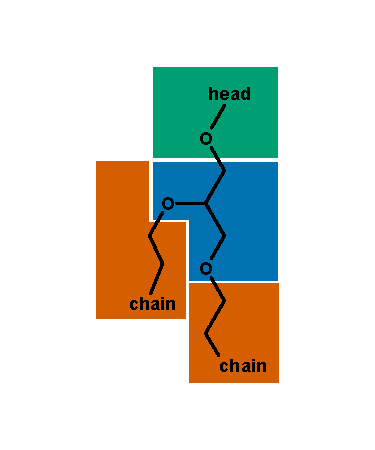
\includegraphics[width=1\linewidth]{figs_ch1/DEG}
        	\caption{DEG}
        \label{fig:DEG}
    \end{subfigure}
    \begin{subfigure}[b]{.3\linewidth}
    	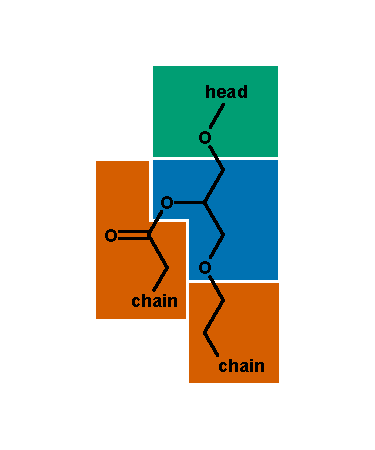
\includegraphics[width=1\linewidth]{figs_ch1/AEG}
    	\caption{AEG}
        \label{fig:AEG}
    \end{subfigure}
    \begin{subfigure}[b]{.3\linewidth}
        	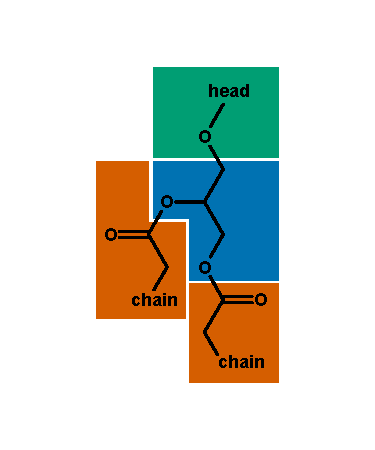
\includegraphics[width=\linewidth]{figs_ch1/DAG}
    	\caption{DAG}
        \label{fig:DAG}
    \end{subfigure}
    \begin{subfigure}[b]{.3\linewidth}
    	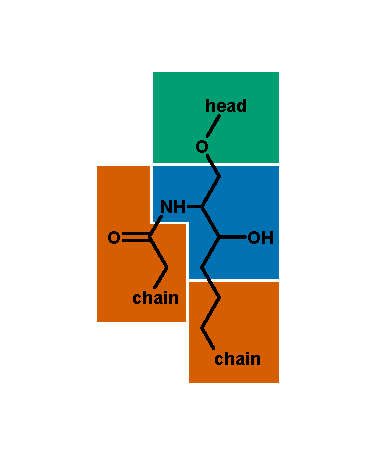
\includegraphics[width=\linewidth]{figs_ch1/CER}
    	\caption{CER}
        \label{fig:CER}
    \end{subfigure}
    \begin{subfigure}[b]{.3\linewidth}
    	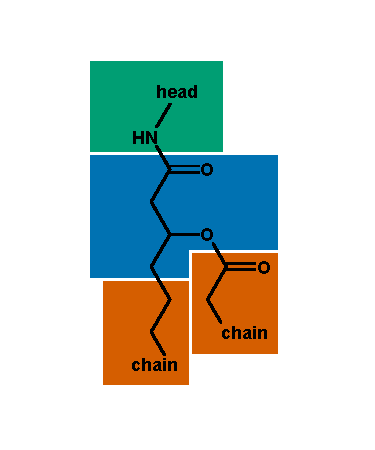
\includegraphics[width=\linewidth]{figs_ch1/FAHFAm}
    	\caption{FAHFAm}
        \label{fig:FAHFAm}
    \end{subfigure}
    \begin{subfigure}[b]{.3\linewidth}
        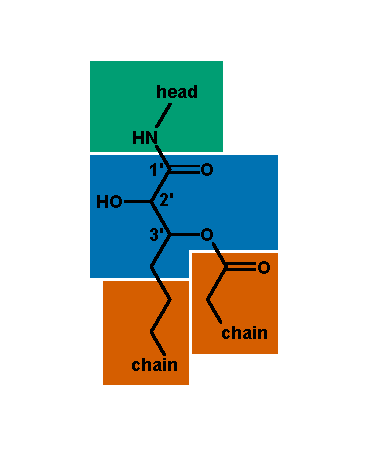
\includegraphics[width=\linewidth]{figs_ch1/FAHFAm-OH}
    	\caption{FAHFAm-OH*}
        \label{fig:FAHFAm-OH}
    \end{subfigure}
    \begin{subfigure}[b]{.6\linewidth}
        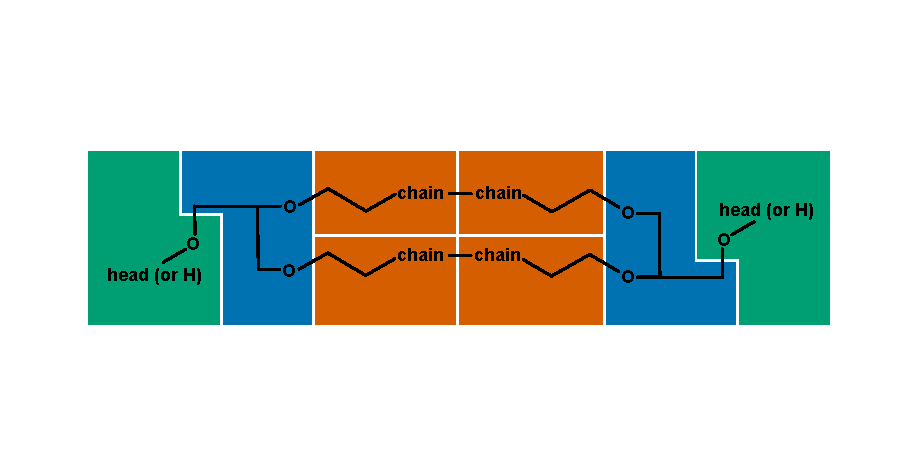
\includegraphics[width=\linewidth]{figs_ch1/GDGT}
    	\caption{GDGT}
        \label{fig:GDGT}
    \end{subfigure}
    \begin{subfigure}[b]{.3\linewidth}
    	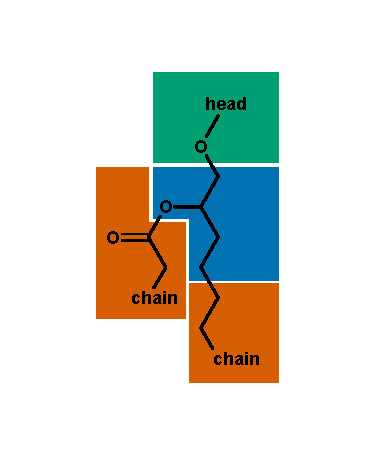
\includegraphics[width=\linewidth]{figs_ch1/alkanediol}
    	\caption{1,2-alkanediol}
        \label{fig:diol}
    \end{subfigure}
\end{figure}
\newpage
\begin{figure}[h]\ContinuedFloat

    \begin{subfigure}[b]{.3\linewidth}
    	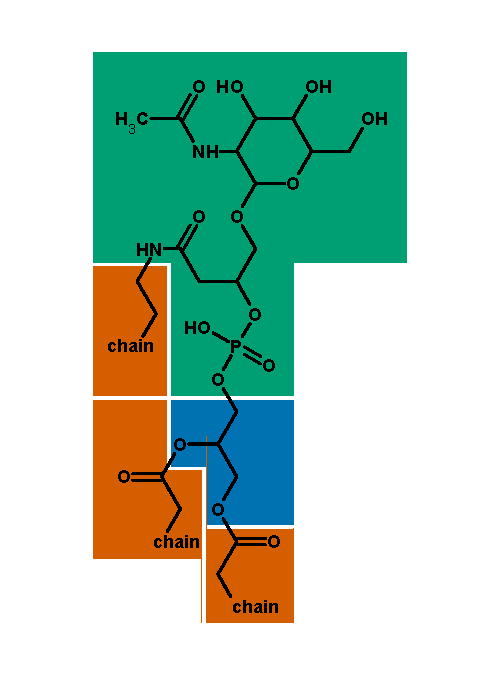
\includegraphics[width=\linewidth]{figs_ch1/NAcG-P-DAG}
    	\caption{NAcG-P-DAG}
        \label{fig:NAcG-P-DAG}
    \end{subfigure}
    \begin{subfigure}[b]{.3\linewidth}
    	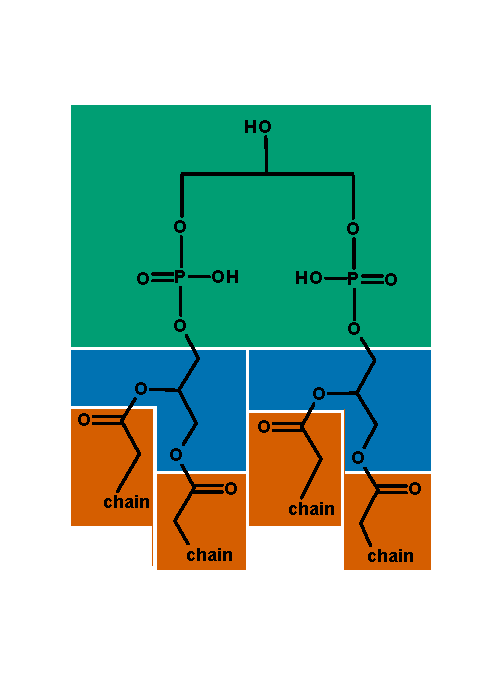
\includegraphics[width=\linewidth]{figs_ch1/DPG}
    	\caption{DPG}
        \label{fig:DPG}
    \end{subfigure}
    \begin{subfigure}[b]{.3\linewidth}
        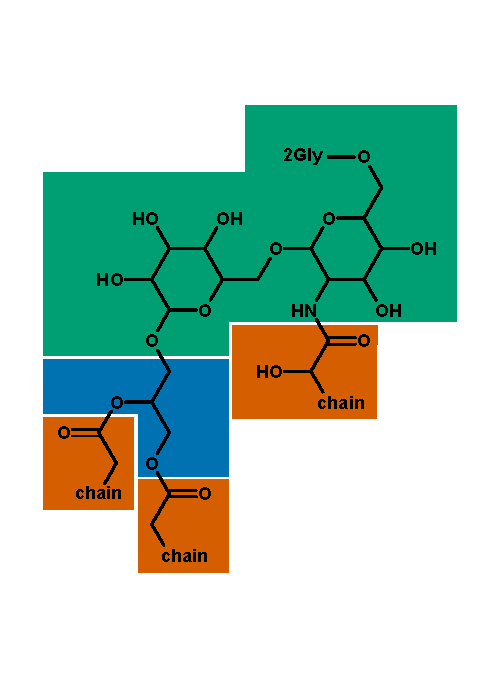
\includegraphics[width=\linewidth]{figs_ch1/2GNAcG-G-DAG}
    	\caption{2GNAcG-G-DAG**}
        \label{fig:2GNAcG-G-DAG}
    \end{subfigure}

    
\caption[Structural designations used for IPL headgroups, backbones, and alkyl chains]{Structural designations used for IPL headgroups, backbones, and alkyl chains, for the sake of calculating abundance-weighted average properties and chemical formulas. Abbreviations are defined in the text. Green boxes contain elemental abundances associated with headgroups, with only the headgroup-backbone connector group explicitly shown and the rest of the headgroup represented as `head'. The chemical formulae listed in Table \ref{tab:IPL} represent elemental abundances of structures contained within the green box. Blue boxes contain backbone elemental abundances. Orange boxes designate elemental abundances belonging to alkyl chains. Only the chemical structure of the first two carbons of each alkyl chain are shown; with `chain' representing the rest. *In FAHFAm-OH, backbone-alkyl chain esterification may occur on either the 2' or 3' hydroxyl group \citep{diercks2015accumulation}. **Referred to as NAcG-DAG in \cite{schubotz2013spatial}}
\label{fig:IPLdivision}
\end{figure}
\doublespace
\clearpage
}


% % These components have been categorized into three major structural motifs; headgroups, backbones, and alkyl chains. Backbones linked to alkyl chains are referred to here as `tailgroups'. 

% % When considering differences in these motifs across lipid structures, it becomes important to define boundaries between these components for the sake of consistently comparing properties that depend on chemical formulas (such as Z\textsubscript{C} or alkyl chain length), particularly for IPLs without a `traditional' glycerol backbone, such as 1,2-alkanediols, CER-lipids, and FAHFAm-lipids (Figure \ref{fig:diol}, \subref{fig:CER}, and \subref{fig:FAHFAm}/\subref{fig:FAHFAm-OH}, respectively). Described below are the definitions applied to all observed IPL structures to designate chemical formulae of headgroup, backbone, and alkyl chains.

The portion of an IPL comprising a headgroup was structurally designated as one or more covalently bonded polar moieties linked to one or more backbones and is represented by structures contained within green boxes in Figure \ref{fig:IPLdivision}. In some cases, the headgroup itself may be directly linked to one or more alkyl chains, such as in the tentative structures shown in Figures \ref{fig:NAcG-P-DAG} and \ref{fig:2GNAcG-G-DAG}. To calculate consistent chemical formulae, headgroups include electronegative atoms linking them to backbones or chains, such as the oxygen atom that forms the glycosidic bond between backbone and sugar headgroup in a glycolipid. Furthermore, the chemical formulae of all headgroups are calculated for their neutrally charged state, with the +1 charge imparted by quaternary ammonium functional of cationic lipids PC, TM-OL, TM-OL-OH, and TM-KL serving as the only exception because this charge was not the result of pH-dependent ionization.

Backbone structures are designated by blue boxes in Figure \ref{fig:IPLdivision}. In this study, IPL backbones were structurally designated according to three criteria chosen to promote consistency between observed IPL structures. First, the backbone must have a linear aliphatic chain of three carbons. Second, one carbon must be covalently bonded to an IPL headgroup. Third, the backbone must include two `connector' functional groups that serve to anchor alkyl chains. Various backbone-alkyl chain linkage types are shown in Figure \ref{fig:chain_comparison}, with backbone connector groups shown proximal to the R\textsubscript{1} group representing the rest of the backbone; -CH$_{2}$- for a carbon-carbon (C-C) link (\textit{e.g.} Figure \ref{fig:chain_comparison}a), -O- for an ether link (\textit{e.g.} Figure \ref{fig:chain_comparison}b, c, d, and e), -NH- for an amide link (\textit{e.g.} Figure \ref{fig:chain_comparison}f), or -O- for an ester link (\textit{e.g.} Figure \ref{fig:chain_comparison}g, h, i, and j). The decision to include connector groups in the structure of the backbone rather than in alkyl chains was made to maintain consistency when calculating nC in alkyl chains with C-C backbone-chain linkage relative to other chains. To demonstrate this point, consider the C-C linked alkyl chain 'a' in Figure \ref{fig:chain_comparison} and the ether-linked alkyl chain 'b' in Figure \ref{fig:chain_comparison}. Both are saturated and have approximately the same physical length. To ensure that both chains have the same value for nC, the `connector' groups proximal to the rest of the backbone, R\textsubscript{1}, must be categorized as part of the backbone structure.

\afterpage{
\singlespace
\begin{figure}
\centering
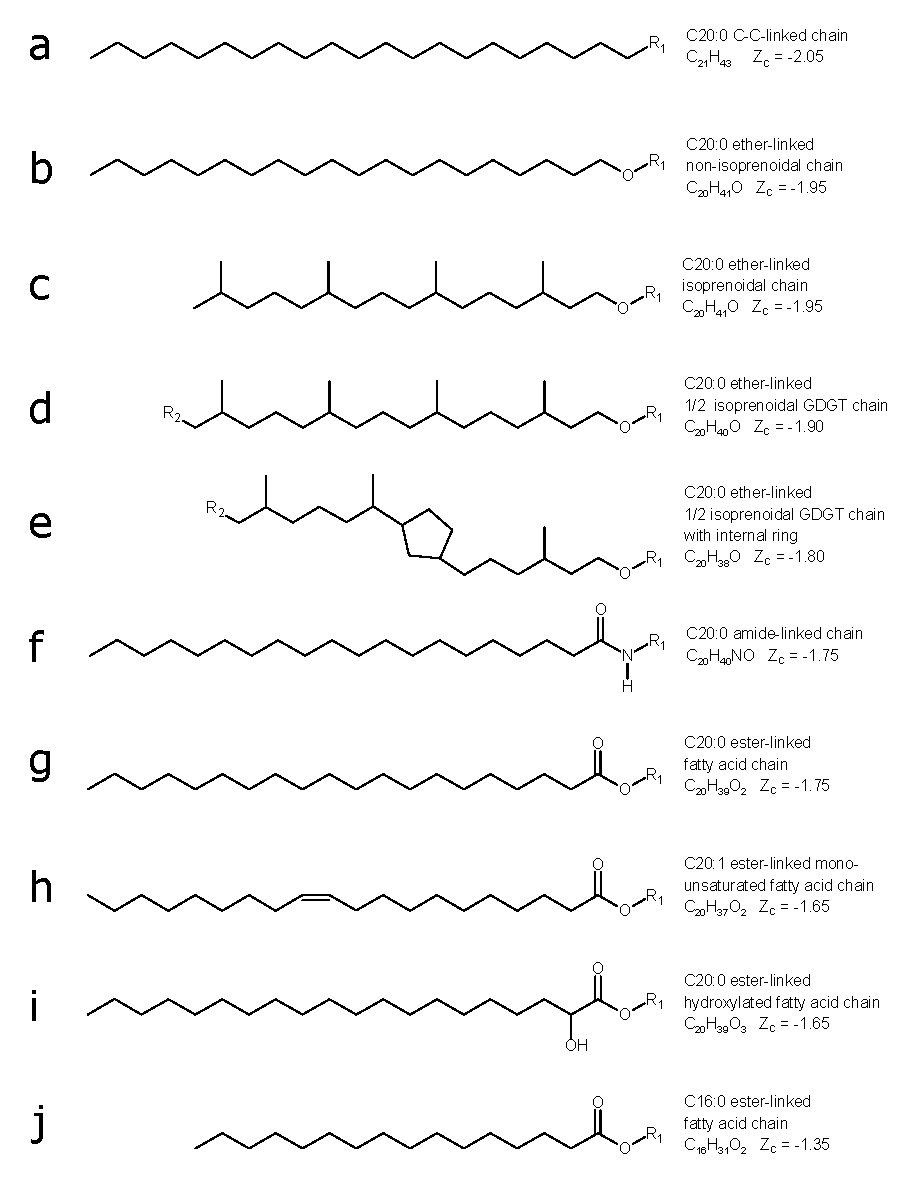
\includegraphics[width=.85\linewidth]{figs_ch1/chain_comparison}
\caption[Lipid alkyl chain modifications and backbone-chain linkage types organized by Z\textsubscript{C}]{Lipid alkyl chain modifications and backbone-chain linkage types organized by Z\textsubscript{C} from reduced (top) to oxidized (bottom). Example structures were chosen to permit comparison of Z\textsubscript{C} according to a various types of biochemical modifications: chain-backbone linkage type as C-C, ether, amide, or ester (a, b, f, g); non-branching and branching chains (b, c); bilayer- and monolayer-forming isoprenoidal chains (c, d); GDGT chains without and with an internal ring (d, e); saturated and unsaturated chains (g, h); non-hydroxylated and hydroxylated chains (g, i); and chains with a greater and lesser number of aliphatic carbons (g, j). R\textsubscript{1} represents the rest of the lipid backbone, and R\textsubscript{2} indicates the second half of a monolayer-forming GDGT chain and was considered a separate chain when calculating average chain properties.}
\label{fig:chain_comparison}
\end{figure}
\doublespace
}

In addition to these two connector groups, the three-carbon backbone may include modifications such as hydroxylations or carbonyl groups. A single lipid may have more than one backbone, such as DPG or GDGT (Figure \ref{fig:DPG} and \ref{fig:GDGT}). 
% For `lyso'-IPLs with only one alkyl chain, the backbone was assigned one extra hydrogen atom to cap off the naked connector group.

Alkyl chains are aliphatic hydrocarbon chains linked to the IPL backbone or in some cases, directly to the headgroup. Their structural designation is indicated by orange boxes in Figure \ref{fig:IPLdivision}. To calculate consistent nC across all observed variations in IPL structure, each chain begins at the carbon directly after the backbone `connector' group and continues to the distal methyl group that caps the end of the chain. Alkyl chains of GDGTs provide the only exception to this, as they have two continuous monolayer-forming (membrane-spanning) isoprenoidal chains rather than two bilayer-forming chains common to non-GDGT IPLs. To calculate and compare chain properties across monolayer and bilayer-forming IPLs, each mole of GDGT was counted as having four moles of equal-length monolayer-forming chains (see Figure \ref{fig:GDGT}), with each chain covalently bonded to one other chain by a -CH\textsubscript{2}- group (\textit{e.g.} Figure \ref{fig:chain_comparison}d or e).





\subsection{Calculation of average lipid properties and elemental composition}
Abundance-weighted properties of IPL headgroups, backbones, and chains were calculated for a sample using the equation

\begin{equation} \label{eq:avecomponent}
\Xi = \frac{\sum_{i} \Xi_{ipl,i} \cdot x_{i}}{\sum_{i} n_{component,i} \cdot x_{i}},
\end{equation}

\noindent where $\Xi$ indicates the average property of interest, $\Xi_{ipl,i}$ represents the property summed across all components in the $i^{th}$ IPL with a mole fraction of $x_{i}$ and $n_{component,i}$ number of the component of interest.

Abundance-weighted properties calculated in this way include nC, nUnsat, and the number of hydroxylations (nOH) per alkyl chain, the fraction of alkyl chains that form monolayers ($x_{monolayer}$), and the fraction backbone-alkyl chain linkage types with an ether ($x_{ether}$), ester ($x_{ester}$), amide ($x_{amide}$), or C-C ($x_{C-C}$) bond.

The abundance-weighted number of internal rings per GDGT (not per alkyl chain) in a sample was also calculated using Equation \ref{eq:avecomponent} by setting $x_{i}$ to the mole fraction of the $i^{th}$ GDGT (rather than the $i^{th}$ IPL), and setting $n_{component,i} \cdot x_{i}$ equal to 1, thereby producing a per-GDGT property and not a per-chain property.

Average chemical formulae of IPL components were determined using known charge and elemental abundance of carbon, hydrogen, nitrogen, oxygen, phosphorus, and sulfur atoms in the chemical structures as $\Xi_{ipl,i}$ in Equation \ref{eq:avecomponent} and then solving for the weighted average of each. The average chemical formulae of full IPL structures were calculated using the charge and elemental abundance summed across the $i^{th}$ IPL while setting $n_{component,i} \cdot x_{i}$ equal to 1. Even when the structure of an IPL component was unclear (\textit{e.g.} the unidentified `223' headgroup observed in this study), its elemental composition was typically obtainable with accurate-mass spectrometry. This permits the inclusion of ambiguous structures when calculating average elemental abundances.

\subsection{Calculation of IPL Z\textsubscript{C}}
Abundance-weighted $Z_{C}$ for IPLs and their component parts were calculated using the abundance-weighted chemical formulae in the equation

\begin{equation} \label{eq:ZC}
{Z}_{C} = \frac{2o + 3n - 5p - 4s - h - Z}{c},
\end{equation}

\noindent where $Z$ stands for the net charge and $c$, $h$, $n$, $o$, $p$, and $s$ represent the number of atoms of carbon, hydrogen, nitrogen, oxygen, phosphorus, and sulfur in the chemical formula of interest. Hydrogen, oxygen, and nitrogen were assigned oxidation states of +1, -2, and -3. Sulfur within the sulfonic acid group of SQ-DAG was assigned an oxidation state of +4. Phosphorus was assigned an oxidation state of +5 to be consistent with that of phosphorus within the phosphate ion. Charge gained or lost by pH-dependent protonation or deprotonation, as is common in many lipid headgroups, does not require extra consideration, as this does not affect $Z_{C}$.

Equation \ref{eq:ZC} was also used to determine the Z\textsubscript{C} values of individual lipid structures, such as those reported in Figure \ref{fig:chain_comparison}.

\subsection{Simulation of analytical uncertainty} A Monte Carlo-style bootstrap sensitivity analysis was performed in which manually integrated IPL HPLC-MS peak areas were allowed to vary randomly by up to 30\% their original value, and analytical response factors applied to any headgroup-backbone combination listed in Table \ref{tab:IPL} were allowed to vary by up two orders of magnitude higher or lower over the course of 999 iterations. Abundance-weighted Z\textsubscript{C} for lipids and their components were re-calculated from abundance-weighted average chemical formulae after each iteration.


\section{Results}

\afterpage{

\singlespace
\begin{table}[htbp]
\begin{adjustbox}{width=\textwidth,keepaspectratio}
\begin{threeparttable}
  \caption{Selected geochemical and physical data from each sample site}
    % Table generated by Excel2LaTeX from sheet 'Geochemical and Physical Data'
% Table generated by Excel2LaTeX from sheet 'Geochemical and Physical Data'
\begin{tabular}{clccrcccc}
\toprule
      &       & \multicolumn{2}{c}{12T UTM coords.} & Dist\tnote{a} & Zone\tnote{b} & Temperature & pH    & Conductivity\tnote{c} \\
\cmidrule{3-4}Site  & Sample & easting & northing & (m)   &       & ($\degree$C) &       & ($\mu$S) \\
\midrule
Bison & BP1   & 510710 & 4935155 & 2.9   & C     & 89.0  & 7.23  & 1550 \\
Pool  & BP2   & 510715 & 4935156 & 8.2   & C     & 80.9  & 7.34  & 1568 \\
      & BP3   & 510718 & 4935157 & 11.1  & T     & 73.3  & 7.27  & 1540 \\
      & BP4   & 510719 & 4935159 & 13.4  & P     & 63.1  & 8.09  & - \\
      & BP5   & 510719 & 4935163 & 17.2  & P     & 40.5  & 8.25  & 1508 \\
      & BP6   & 510724 & 4935165 & 22.6  & P     & 29.0  & 9.01  & 1697 \\
      &       &       &       &       &       &       &       &  \\
Mound & MS1   & 511114 & 4934621 & 3.6   & C     & 91.0  & 8.81  & 1612 \\
Spring & MS2   & 511108 & 4934624 & 12.7  & C     & 77.3  & 8.65  & 1621 \\
      & MS3   & 511098 & 4934628 & 24.2  & P     & 64.8  & 9.08  & 1617 \\
      & MS4   & 511083 & 4934621 & 38.7  & P     & 53.0  & 9.22  & 1634 \\
      & MS5   & 511049 & 4934625 & 53    & P     & 35.1  & 9.53  & 1660 \\
      &       &       &       &       &       &       &       &  \\
Empress & EP1   & 0521589 & 4948280 & 2.2   & C     & 82.2  & 5.78  & 1824 \\
Pool  & EP2   & 0521585 & 4948280 & 6.2   & T     & 70.5  & 6.96  & 1832 \\
      & EP3   & 0521580 & 4948285 & 13.3  & T     & 60.7  & 7.63  & 1840 \\
      & EP4   & 0521560 & 4948293 & 34.8  & P     & 51.6  & 7.99  & 1860 \\
      & EP5   & 0521558 & 4948295 & 37.6  & P     & 38.1  & 8.42  & 1664 \\
      &       &       &       &       &       &       &       &  \\
Octopus & OS1   & 0516054 & 4931217 & 7.0   & C     & 85.4  & 7.29  & 1622 \\
Spring & OS2   & 0516016 & 4931212 & 38.3  & P     & 59.8  & 8.27  & 1581 \\
\bottomrule
\end{tabular}%

    \begin{tablenotes}
      \small
      \item[a] Distance from hot spring source.
      \item[b] Major metabolic regime representative of the microbial community at the sample site, interpreted visually in the field based on the presence or absence of photosynthetic pigments; C, strictly chemosynthetic; T, transition to phototrophy; P, photosynthetic.
      \item[c] Conductivity was normalized to 25\degree C using the formula Cond$_{T}/(1+\alpha(T-25))$, where Cond$_{T}$ was the conductivity measured at the temperature of the sample site and $\alpha$ was the temperature correction coefficient taken as 0.02 for freshwater.
    %   \item[d] Oxygen-18 isotope ratio relative to VSMOW.
    \end{tablenotes}
  \label{tab:geophysical}%
  \end{threeparttable}
  \end{adjustbox}
\end{table}%
\doublespace
\clearpage
}




\afterpage{
\singlespace
\begin{table}[htbp]
  \begin{adjustbox}{width=\textwidth,keepaspectratio}
  \begin{threeparttable}
  \caption[Concentrations of selected redox-sensitive dissolved chemical species]{Concentrations of selected redox-sensitive dissolved chemical species\textsuperscript{a}}


% Table generated by Excel2LaTeX from sheet 'Geochemical and Physical Data'
\begin{tabular}{clrrrrrr}
\toprule
      &       & \multicolumn{4}{c}{Oxidized}  & \multicolumn{2}{c}{Reduced} \\
\cmidrule(l{2pt}r{2pt}){3-6} \cmidrule(l{2pt}r{2pt}){7-8}      &       & \multicolumn{1}{c}{O\textsubscript{2}} & \multicolumn{1}{c}{NO\textsubscript{3}\textsuperscript{-}} & \multicolumn{1}{c}{NO\textsubscript{2}\textsuperscript{-}} & \multicolumn{1}{c}{$\sum$SO\textsubscript{4}\textsuperscript{2-}} & \multicolumn{1}{c}{$\sum$NH\textsubscript{4}\textsuperscript{+}} & \multicolumn{1}{c}{$\sum$HS\textsuperscript{-}} \\
Site  & Sample & \multicolumn{1}{c}{(mg l\textsuperscript{-1})} & \multicolumn{1}{c}{(mg l\textsuperscript{-1})} & \multicolumn{1}{c}{(mg l\textsuperscript{-1})} & \multicolumn{1}{c}{(mg l\textsuperscript{-1})} & \multicolumn{1}{c}{(mg l\textsuperscript{-1})} & \multicolumn{1}{c}{($\mu$g l\textsuperscript{-1})} \\
\midrule
Bison & BP1   & 0.2   & 0.01  & 0.02  & 13.11 & 0.07  & 230 \\
Pool  & BP2   & 0.7   & 0.01  & 0.04  & 15.43 & 0.06  & 220 \\
      & BP3   & 1.1   & 0.02  & 0.01  & 16.81 & 0.04  & bdl\tnote{b} \\
      & BP4   & 2.3   & 0.03  & 0.02  & 16.50 & 0.02  & 6 \\
      & BP5   & 5.7   & 0.004 & bdl   & 17.18 & 0.01  & 15 \\
      & BP6   & 3.3   & 0.07  & bdl   & 18.32 & 0.02  & 10 \\
      &       &       &       &       &       &       &  \\
Mound & MS1   & 0.4   & 0.01  & bdl   & 14.33 & 0.07  & 716 \\
Spring & MS2   & 2.2   & 0.01  & bdl   & 15.03 & 0.01  & 758 \\
      & MS3   & 1.4   & 0.04  & 0.02  & 16.99 & 0.03  & 236 \\
      & MS4   & 3.6   & 0.02  & 0.01  & 17.56 & 0.02  & 70 \\
      & MS5   & 6.9   & 0.06  & bdl   & 20.11 & bdl   & bdl \\
      &       &       &       &       &       &       &  \\
Empress & EP1   & 0.4   & 0.01  & 0.08  & 106.87 & 0.42  & 260 \\
Pool  & EP2   & 0.7   & -     & -     & -     & -     & 97 \\
      & EP3   & 1.2   & 0.01  & bdl   & 106.70 & 0.31  & 37 \\
      & EP4   & 1.3   & 0.03  & 0.03  & 111.70 & 0.39  & 31 \\
      & EP5   & 3.4   & 0.08  & 0.01  & 111.24 & 0.14  & 18 \\
      &       &       &       &       &       &       &  \\
Octopus & OS1   & 0.5   & 0.03  & 0.03  & 17.82 & 0.06  & 13 \\
Spring & OS2   & 3.3   & 0.03  & 0.02  & 18.76 & 0.02  & 12 \\
\bottomrule
\end{tabular}%


	\begin{tablenotes}
      \small
      \item[a] Note: Sulfide (HS\textsuperscript{-}), ammonium (NH\textsubscript{4}\textsuperscript{+}), and sulfate (SO\textsubscript{4}\textsuperscript{2-}) concentrations are summed for their respective pH-dependent protonated states.
      
      \item[b] bdl: below detection limit
      \normalsize
    \end{tablenotes}
  \label{tab:redox}%
  \end{threeparttable}
  \end{adjustbox}
\end{table}%
\doublespace
% to get nicer header midrules, replace \cmidrule{3-8} with
% \cmidrule(l{2pt}r{2pt}){3-6} \cmidrule(l{2pt}r{2pt}){7-8}
\clearpage
}

\afterpage{
\singlespace
\begin{figure}[h]
\centering
\includegraphics[width=1\linewidth]{"figs_ch1/scatterplot - hot spring redox"}
\caption[Total concentrations of redox-sensitive aqueous chemical species in samples from Bison Pool, Mound Spring, Empress Pool, and Octopus Spring]{Total concentrations of redox-sensitive aqueous chemical species in samples from Bison Pool (A), Mound Spring (B), Empress Pool (C) and Octopus Spring (D). Lines between points are meant to guide the eye between measurements only. A water sample was not collected for sulfate at Empress Pool site EP2 during the 2012 field season, indicated here by a dashed line between sulfate measurements for sites EP1 and EP3.}
\label{fig:redox}
\end{figure}
\doublespace
\clearpage
}


\subsection{Water chemistry and redox potential} Temperature, pH, and conductivity measurements corresponding to samples along the four studied hot spring outflow channels are shown in Table \ref{tab:geophysical}. As water flows from the source and cools, microbial communities in alkaline hot springs change spatially along the channel, with chemotrophs dominating the higher-temperature end and green/orange pigmented phototrophic cyanobacteria at the lower-temperature end. All four studied outflow channels show downstream changes in water chemistry as shown in Table \ref{tab:redox}, which in all cases are marked by an overall decrease in concentration of reduced inorganic dissolved species and an increase in the concentration of oxidized inorganic solutes. It can be seen from Figure \ref{fig:redox} that concentrations of relatively reduced sulfide are more concentrated at the source and gradually give way to its oxidized counterpart sulfate, likely due to biological oxidation \citep{cox2011transition}. Previous research at Bison Pool and Mound Spring by \cite{loiacono2012evidence} demonstrated active expression of nitrogen-metabolizing genes by nitrifying microorganisms, likely explaining the downstream decrease of ammonia concentrations and a concurrent increase in nitrite and nitrate concentrations reported in Table \ref{tab:redox}. The dissolved oxygen also exhibits an overall increase in concentration downstream, which can likely be attributed to flowing water mixing with the atmosphere, as well as input from oxygenic photosynthesis after the onset of cyanobacteria. Taken together, these geochemical data suggest that the redox potential of the water was generally more reduced at the hot spring source and gradually becomes more oxidized downstream.


\afterpage{
% \newgeometry{margin=1.5cm} % modify this if you need even more space
\begin{landscape}
\singlespace

\begin{table}
\centering
\normalsize
\begin{adjustbox}{width=600pt,keepaspectratio}
\begin{threeparttable}
  \caption{Weighted Z\textsubscript{C} and chemical formula of IPLs and their component parts}
 % to get nicer header midrules, replace \cmidrule{3-10} with
% \cmidrule(l{2pt}r{2pt}){3-6} \cmidrule(l{2pt}r{2pt}){7-10}


% Table generated by Excel2LaTeX from sheet 'ZC and chain formulae'
\begin{tabular}{lccccccccc}
\toprule
      &       & \multicolumn{4}{c}{Weighted Z\textsubscript{C}} & \multicolumn{4}{c}{Weighted chemical formula} \\
\cmidrule(l{2pt}r{2pt}){3-6} \cmidrule(l{2pt}r{2pt}){7-10}Site  & Sample & Full IPLs & Headgroups & Backbones & Alkyl chains & Full IPLs & Headgroups & Backbones & Alkyl chains \\
\midrule
Bison & BP1   & -1.56 & 0.15  & -0.34 & -1.92 & C\textsubscript{64.1}H\textsubscript{123.}N\textsubscript{2.15e-1}O\textsubscript{12.3}P\textsubscript{5.01e-1}S\textsubscript{1.27e-3}\textsuperscript{+8.04e-3} & C\textsubscript{5.61}H\textsubscript{11.0}N\textsubscript{1.46e-1}O\textsubscript{6.70}P\textsubscript{3.95e-1}S\textsubscript{9.55e-4}\textsuperscript{+6.07e-3} & C\textsubscript{3.02}H\textsubscript{5.05}N\textsubscript{1.71e-2}O\textsubscript{1.99} & C\textsubscript{19.8}H\textsubscript{38.5}O\textsubscript{2.85e-1} \\
Pool  & BP2   & -1.53 & 0.15  & -0.34 & -1.89 & C\textsubscript{56.9}H\textsubscript{109.}N\textsubscript{2.10e-1}O\textsubscript{12.3}P\textsubscript{6.07e-1}S\textsubscript{2.42e-3}\textsuperscript{+1.42e-2} & C\textsubscript{6.25}H\textsubscript{12.1}N\textsubscript{1.58e-1}O\textsubscript{7.62}P\textsubscript{5.34e-1}S\textsubscript{2.05e-3}\textsuperscript{+1.21e-2} & C\textsubscript{3.04}H\textsubscript{5.07}N\textsubscript{2.25e-2}O\textsubscript{1.99} & C\textsubscript{19.4}H\textsubscript{37.6}O\textsubscript{4.36e-1} \\
      & BP3   & -1.45 & 0.11  & -0.35 & -1.84 & C\textsubscript{48.0}H\textsubscript{91.5}N\textsubscript{1.48e-1}O\textsubscript{12.1}P\textsubscript{5.31e-1}S\textsubscript{8.32e-2}\textsuperscript{+4.61e-3} & C\textsubscript{6.71}H\textsubscript{12.9}N\textsubscript{1.03e-1}O\textsubscript{8.10}P\textsubscript{5.12e-1}S\textsubscript{7.95e-2}\textsuperscript{+4.40e-3} & C\textsubscript{3.06}H\textsubscript{5.12}N\textsubscript{3.89e-2}O\textsubscript{1.97} & C\textsubscript{17.9}H\textsubscript{34.5}O\textsubscript{7.54e-1} \\
      & BP4   & -1.46 & 0.13  & -0.35 & -1.88 & C\textsubscript{45.1}H\textsubscript{86.8}N\textsubscript{8.39e-2}O\textsubscript{12.1}P\textsubscript{6.25e-1}S\textsubscript{5.38e-2}\textsuperscript{+8.07e-3} & C\textsubscript{7.22}H\textsubscript{13.7}N\textsubscript{5.44e-2}O\textsubscript{8.90}P\textsubscript{6.23e-1}S\textsubscript{5.36e-2}\textsuperscript{+8.04e-3} & C\textsubscript{3.04}H\textsubscript{5.09}N\textsubscript{2.91e-2}O\textsubscript{1.97} & C\textsubscript{17.3}H\textsubscript{33.7}O\textsubscript{5.67e-1} \\
      & BP5   & -1.38 & 0.04  & -0.32 & -1.80 & C\textsubscript{44.6}H\textsubscript{83.7}N\textsubscript{3.32e-1}O\textsubscript{11.4}P\textsubscript{2.17e-1}S\textsubscript{1.21e-1}\textsuperscript{+1.24e-1} & C\textsubscript{7.82}H\textsubscript{14.6}N\textsubscript{3.26e-1}O\textsubscript{7.69}P\textsubscript{2.17e-1}S\textsubscript{1.21e-1}\textsuperscript{+1.24e-1} & C\textsubscript{3.11}H\textsubscript{5.02}N\textsubscript{5.65e-3}O\textsubscript{2.01} & C\textsubscript{16.8}H\textsubscript{32.0}O\textsubscript{8.49e-1} \\
      & BP6   & -1.36 & 0.02  & -0.33 & -1.73 & C\textsubscript{43.5}H\textsubscript{80.4}N\textsubscript{2.70e-1}O\textsubscript{11.6}P\textsubscript{4.64e-1}S\textsubscript{1.18e-1}\textsuperscript{+8.39e-2} & C\textsubscript{6.67}H\textsubscript{13.1}N\textsubscript{2.63e-1}O\textsubscript{7.57}P\textsubscript{4.63e-1}S\textsubscript{1.18e-1}\textsuperscript{+8.37e-2} & C\textsubscript{3.04}H\textsubscript{5.02}N\textsubscript{6.73e-3}O\textsubscript{2.00} & C\textsubscript{16.7}H\textsubscript{30.8}O\textsubscript{9.75e-1} \\
      &       &       &       &       &       &       &       &       &  \\
Mound & MS1   & -1.68 & 0.32  & -0.33 & -1.94 & C\textsubscript{92.2}H\textsubscript{177.}N\textsubscript{4.49e-4}O\textsubscript{11.2}P\textsubscript{2.43e-4}\textsuperscript{+7.34e-6} & C\textsubscript{3.14}H\textsubscript{6.23}N\textsubscript{1.29e-4}O\textsubscript{3.61}P\textsubscript{1.22e-4}\textsuperscript{+3.67e-6} & C\textsubscript{3.00}H\textsubscript{5.00}N\textsubscript{9.56e-5}O\textsubscript{2.00} & C\textsubscript{20.0}H\textsubscript{38.8}O\textsubscript{3.52e-4} \\
Spring & MS2   & -1.61 & 0.18  & -0.38 & -1.93 & C\textsubscript{68.7}H\textsubscript{133.}N\textsubscript{2.22e-1}O\textsubscript{12.0}P\textsubscript{3.77e-1}S\textsubscript{2.10e-2}\textsuperscript{+4.40e-3} & C\textsubscript{5.12}H\textsubscript{9.87}N\textsubscript{7.51e-2}O\textsubscript{5.98}P\textsubscript{2.65e-1}S\textsubscript{1.46e-2}\textsuperscript{+3.06e-3} & C\textsubscript{3.09}H\textsubscript{5.24}N\textsubscript{8.02e-2}O\textsubscript{1.92} & C\textsubscript{19.6}H\textsubscript{38.2}O\textsubscript{2.12e-1} \\
      & MS3   & -1.52 & 0.14  & -0.35 & -1.92 & C\textsubscript{49.9}H\textsubscript{96.5}N\textsubscript{4.98e-2}O\textsubscript{11.9}P\textsubscript{6.47e-1}S\textsubscript{2.03e-2}\textsuperscript{+1.27e-3} & C\textsubscript{6.57}H\textsubscript{12.6}N\textsubscript{1.72e-2}O\textsubscript{8.26}P\textsubscript{5.94e-1}S\textsubscript{1.86e-2}\textsuperscript{+1.17e-3} & C\textsubscript{3.03}H\textsubscript{5.09}N\textsubscript{2.84e-2}O\textsubscript{1.97} & C\textsubscript{18.0}H\textsubscript{35.3}O\textsubscript{3.30e-1} \\
      & MS4   & -1.43 & 0.06  & -0.34 & -1.82 & C\textsubscript{47.2}H\textsubscript{89.6}N\textsubscript{2.07e-1}O\textsubscript{12.1}P\textsubscript{4.93e-1}S\textsubscript{5.34e-2}\textsuperscript{+5.00e-2} & C\textsubscript{7.20}H\textsubscript{13.8}N\textsubscript{1.91e-1}O\textsubscript{8.12}P\textsubscript{4.78e-1}S\textsubscript{5.18e-2}\textsuperscript{+4.85e-2} & C\textsubscript{3.03}H\textsubscript{5.03}N\textsubscript{9.59e-3}O\textsubscript{1.99} & C\textsubscript{17.4}H\textsubscript{33.3}O\textsubscript{7.89e-1} \\
      & MS5   & -1.33 & -0.07 & -0.34 & -1.71 & C\textsubscript{46.6}H\textsubscript{85.5}N\textsubscript{2.60e-1}O\textsubscript{12.5}P\textsubscript{3.65e-1}S\textsubscript{1.25e-1}\textsuperscript{+1.69e-1} & C\textsubscript{8.29}H\textsubscript{15.9}N\textsubscript{2.51e-1}O\textsubscript{8.36}P\textsubscript{3.62e-1}S\textsubscript{1.24e-1}\textsuperscript{+1.68e-1} & C\textsubscript{3.04}H\textsubscript{5.02}N\textsubscript{7.05e-3}O\textsubscript{1.99} & C\textsubscript{16.8}H\textsubscript{30.7}O\textsubscript{9.51e-1} \\
      &       &       &       &       &       &       &       &       &  \\
Empress & EP1   & -1.60 & 0.22  & -0.33 & -1.96 & C\textsubscript{85.0}H\textsubscript{164.}N\textsubscript{1.17e-1}O\textsubscript{13.8}P\textsubscript{4.38e-2}\textsuperscript{+2.05e-4} & C\textsubscript{5.66}H\textsubscript{10.4}N\textsubscript{6.51e-2}O\textsubscript{5.79}P\textsubscript{2.97e-2}\textsuperscript{+1.16e-4} & C\textsubscript{3.00}H\textsubscript{5.01}N\textsubscript{2.23e-3}O\textsubscript{2.00} & C\textsubscript{19.8}H\textsubscript{38.8}O\textsubscript{1.61e-2} \\
Pool  & EP2   & -1.54 & 0.15  & -0.36 & -1.92 & C\textsubscript{62.0}H\textsubscript{119.}N\textsubscript{1.87e-1}O\textsubscript{12.5}P\textsubscript{4.18e-1}S\textsubscript{1.16e-2}\textsuperscript{+8.26e-3} & C\textsubscript{6.22}H\textsubscript{11.8}N\textsubscript{8.79e-2}O\textsubscript{7.06}P\textsubscript{3.28e-1}S\textsubscript{8.81e-3}\textsuperscript{+6.30e-3} & C\textsubscript{3.07}H\textsubscript{5.17}N\textsubscript{5.52e-2}O\textsubscript{1.95} & C\textsubscript{18.9}H\textsubscript{36.8}O\textsubscript{2.61e-1} \\
      & EP3   & -1.54 & 0.15  & -0.34 & -1.90 & C\textsubscript{67.9}H\textsubscript{130.}N\textsubscript{1.06e-1}O\textsubscript{13.4}P\textsubscript{3.20e-1}S\textsubscript{3.36e-2}\textsuperscript{+1.15e-2} & C\textsubscript{6.11}H\textsubscript{11.5}N\textsubscript{5.37e-2}O\textsubscript{6.74}P\textsubscript{2.32e-1}S\textsubscript{2.34e-2}\textsuperscript{+7.98e-3} & C\textsubscript{3.03}H\textsubscript{5.06}N\textsubscript{2.05e-2}O\textsubscript{1.98} & C\textsubscript{19.1}H\textsubscript{36.9}O\textsubscript{2.95e-1} \\
      & EP4   & -1.44 & 0.08  & -0.33 & -1.83 & C\textsubscript{51.6}H\textsubscript{97.2}N\textsubscript{2.52e-1}O\textsubscript{11.7}P\textsubscript{1.99e-1}S\textsubscript{1.13e-1}\textsuperscript{+8.90e-2} & C\textsubscript{6.88}H\textsubscript{12.9}N\textsubscript{2.11e-1}O\textsubscript{7.00}P\textsubscript{1.78e-1}S\textsubscript{9.96e-2}\textsuperscript{+7.87e-2} & C\textsubscript{3.07}H\textsubscript{5.04}N\textsubscript{1.18e-2}O\textsubscript{2.00} & C\textsubscript{17.8}H\textsubscript{33.9}O\textsubscript{6.78e-1} \\
      & EP5   & -1.37 & -0.01 & -0.31 & -1.77 & C\textsubscript{48.1}H\textsubscript{89.0}N\textsubscript{3.69e-1}O\textsubscript{11.6}P\textsubscript{8.99e-2}S\textsubscript{1.79e-1}\textsuperscript{+1.57e-1} & C\textsubscript{7.78}H\textsubscript{14.6}N\textsubscript{3.44e-1}O\textsubscript{7.23}P\textsubscript{8.53e-2}S\textsubscript{1.68e-1}\textsuperscript{+1.47e-1} & C\textsubscript{3.11}H\textsubscript{5.00}N\textsubscript{1.48e-3}O\textsubscript{2.01} & C\textsubscript{17.1}H\textsubscript{31.9}O\textsubscript{8.12e-1} \\
      &       &       &       &       &       &       &       &       &  \\
Octopus & OS1   & -1.56 & 0.13  & -0.34 & -1.95 & C\textsubscript{64.4}H\textsubscript{125.}N\textsubscript{9.12e-2}O\textsubscript{13.7}P\textsubscript{5.91e-1}S\textsubscript{2.83e-3}\textsuperscript{+1.45e-3} & C\textsubscript{6.97}H\textsubscript{13.3}N\textsubscript{8.14e-2}O\textsubscript{8.32}P\textsubscript{5.36e-1}S\textsubscript{2.23e-3}\textsuperscript{+1.15e-3} & C\textsubscript{3.01}H\textsubscript{5.02}N\textsubscript{5.92e-3}O\textsubscript{1.99} & C\textsubscript{20.4}H\textsubscript{40.3}O\textsubscript{2.63e-1} \\
Spring & OS2   & -1.48 & 0.12  & -0.34 & -1.89 & C\textsubscript{45.2}H\textsubscript{87.3}N\textsubscript{1.01e-1}O\textsubscript{11.9}P\textsubscript{6.79e-1}S\textsubscript{4.19e-2}\textsuperscript{+1.93e-2} & C\textsubscript{6.91}H\textsubscript{13.3}N\textsubscript{8.39e-2}O\textsubscript{8.72}P\textsubscript{6.78e-1}S\textsubscript{4.18e-2}\textsuperscript{+1.93e-2} & C\textsubscript{3.03}H\textsubscript{5.05}N\textsubscript{1.69e-2}O\textsubscript{1.99} & C\textsubscript{17.5}H\textsubscript{34.2}O\textsubscript{5.73e-1} \\
\bottomrule
\end{tabular}%


\begin{tablenotes}

\item
% \item [a] Full IPL structure.
% \item [b] Headgroup structure only.
% \item [c] Backbone structure only.
% \item [d] Alkyl chain structure only.

\end{tablenotes}

  \label{tab:IPL_ZC}
  \end{threeparttable}
  \end{adjustbox}
\end{table}

\end{landscape}
\doublespace
\clearpage
}




\afterpage{
\singlespace
\begin{figure}[h]
\centering
    \begin{subfigure}[b]{0.81\linewidth}
        	\includegraphics[width=1\linewidth]{"figs_ch1/scatterplot - weighted ZC of IPL components vs temp and logO2"}
    \end{subfigure}
    \begin{subfigure}[b]{0.18\linewidth}
        	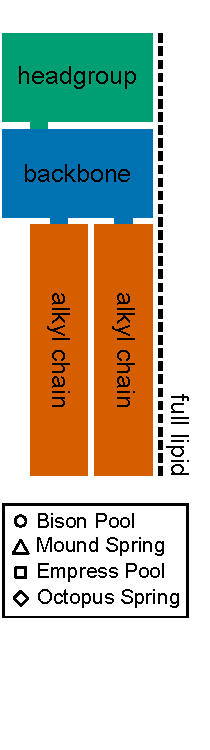
\includegraphics[width=1\linewidth]{figs_ch1/BasicLipidSchematic.pdf}
    \end{subfigure}
\caption[Abundance-weighted Z\textsubscript{C} of IPLs and their component parts]{Abundance-weighted Z\textsubscript{C} of headgroups (green), backbones (blue), alkyl chains (orange) and full (black) thermophile IPLs sampled along the outflow channels of four Yellowstone hot springs with respect to temperature (left) and log molality of dissolved O\textsubscript{2} (right). Observed values of weighted Z\textsubscript{C} of extracted lipids and their components are indicated by points. Bars and best-fit lines show the standard deviation and linear regression of 999 weighted Z\textsubscript{C} resulting from the bootstrap sensitivity analysis. Shaded areas represent 95\% intervals for the prediction of future bootstrap Z\textsubscript{C} values.}
\label{fig:weighted_ZC}
\end{figure}
\doublespace
\clearpage
}

\subsection{Z\textsubscript{C} of IPLs and their components}

The abundance-weighted chemical formulae and Z\textsubscript{C} calculated for thermophilic microbial IPLs and their headgroups, backbones, and alkyl chains are reported in Table \ref{tab:IPL_ZC} for samples collected from Bison Pool, Mound Spring, Empress Pool, and Octopus Spring. As shown in Figure \ref{fig:weighted_ZC}, decreasing temperature and increasingly oxidized conditions coincide with near-linear changes in the weighted Z\textsubscript{C} of IPLs and their components. Carbon was most reduced in IPLs sampled closest to the spring sources (Z\textsubscript{C} between -1.68 and -1.56) where temperatures were highest (82.2 to 91.0$^\circ$C) and concentrations of oxidized inorganic species (nitrate, sulfate, and oxygen) were lowest. In progressively downstream samples, carbon in IPLs became more oxidized, with weighted Z\textsubscript{C} between -1.36 and -1.33 for samples in the 29.0 to 38.1$^\circ$C temperature range where measured concentrations of sulfate, nitrate, and oxygen tended to be greatest. This trend persists even after simulating potential sources of analytical error, as shown in Figure \ref{fig:weighted_ZC} by the black bars above and below the `canon' observations of abundance-weighted Z\textsubscript{C}, which indicate the standard deviation of weighted Z\textsubscript{C} resulting from 999 iterations of the bootstrap sensitivity analysis. The standard deviations of IPL weighted Z\textsubscript{C} show little overlap between upstream and downstream samples after random variation of up to 30\% for integrated HPLC-MS peak areas and up to two orders of magnitude for response factors.

Alkyl chains tend to have weighted Z\textsubscript{C} approximately 0.3-0.4 more negative than those of the full structure regardless of the sample. Compared to headgroups and backbones, the weighted Z\textsubscript{C} of alkyl chains were closest to that of the full structure, implicating this component as the primary contributor to full IPL Z\textsubscript{C} and observed trends with temperature and redox. This agrees with the observation that most carbon in IPLs belongs to the alkyl chains. Since alkyl chains have a high H/C ratio to facilitate their hydrophobicity, the weighted ZC of full IPLs and their chains are significantly more negative than those of backbones and headgroups, which have a higher ratio of electronegative atoms (\textit{e.g.} oxygen, nitrogen) to carbon because of their relative hydrophilicity. As shown by in Figure \ref{fig:weighted_ZC}, trends in alkyl chain Z\textsubscript{C} appear to be more resilient to simulated sources of analytical uncertainty than the full structure based on sample standard deviations and the narrow 95\% prediction interval generated by the bootstrap sensitivity analysis. The width of the prediction interval for future bootstrap results does not overlap between the highest temperature and lowest temperature, which the authors interpret as further evidence observed trends in alkyl chains are not artifacts of the analytical method used to quantify lipid abundance.

The weighted Z\textsubscript{C} of IPL backbones did not change significantly with temperature or redox, as most observed backbones were comprised of glycerol regardless of the sample. According to the IPL component division scheme used in this study, an IPL glycerol backbone has a chemical formula of C\textsubscript{3}H\textsubscript{5}O\textsubscript{2}, corresponding to a Z\textsubscript{C} of $-0.\overline{3}$. This was close to the abundance-weighted value in every sample, with little variation.

Carbon in headgroups was significantly more oxidized than any other component, with weighted Z\textsubscript{C} ranging between -0.01 to 0.32 across samples. Glycolipid headgroups 1G (Z\textsubscript{C} = $0.1\overline{6}$) and 2G (Z\textsubscript{C} = $0.08\overline{3}$) were among the most abundant headgroups observed in all four springs regardless of temperature or redox, though they were most abundant, along with the glycolipid SQ (Z\textsubscript{C} = $0.1\overline{6}$) in samples where photosynthetic microorganisms are visually apparent. This agrees with observations that 1G, 2G, and SQ glycolipids are abundant in cyanobacterial \citep{wada2009lipids} and algal \citep{guschina2006lipids} photosynthetic membranes.

Phosphate-bearing phospholipids and glycophospholipids, especially lipids with PI headgroups, were more abundant downstream than upstream, though the incorporation of phosphate into the glycolipid headgroups had little to no effect on abundance-weighted headgroup Z\textsubscript{C}, as there was no difference in Z\textsubscript{C} between analogous nonphosphorylated and phosphorylated headgroups (\textit{e.g.} no difference in Z\textsubscript{C} between 1G-P and 1G, or between 2G-P and 2G, \textit{etc.}). The greatest abundance of lipids with an APT phospholipid headgroup (Z\textsubscript{C} = -0.2) was observed in `pink streamer' thermophile communities sampled from the upstream chemosynthetic zones of Bison Pool and Octopus Spring, which agrees with previous reports that this lipid is common in streamers dominated by \textit{Aquificales} bacteria \citep{Sturt_Intact_2004, schubotz2013spatial}. However, after applying response factors, the abundance APT was scarce relative to other headgroups, even in streamer samples.

% % Sollich paper: "acyl chains of BL, another well-known component of photosynthetic membranes (Dembitsky, 1996; Kato et al., 1996)"

% % Sollich paper: PC and CL (DPG) are common in mitochondria, and euk membranes tend to be rich with ceramides and sphingomyelin. We don't see much of that at cooler sites, though we tend to see more 'uncommon' phosphate-based PE, PG, PI, therefore we guess that bacteria, and not euk, dominate at those sites.

Intriguingly, weighted Z\textsubscript{C} of IPL headgroups became progressively negative with decreasing temperature or increasingly oxidized conditions, which was the reverse of trends observed alkyl chains and full IPLs. One reason for this stems from the way abundance-weighted Z\textsubscript{C} was calculated for GDGT headgroups. Because of the monolayer-forming properties of GDGTs, one mole of GDGT will have two moles of headgroup. As an example, consider that 1G-GDGT has two headgroups; the first is a glycosyl moiety linked to glycerol one side of the GDGT, and the second is a hydroxyl (-OH) group terminating the glycerol on the other side of the GDGT. Summing the elemental abundances of 1G (C\textsubscript{6}H\textsubscript{11}O\textsubscript{6}) and -OH results in a total of C\textsubscript{6}H\textsubscript{12}O\textsubscript{7} for both headgroups of 1G-GDGT, or C\textsubscript{3}H\textsubscript{6}O\textsubscript{3.5} per headgroup. Accounting for this extra -OH means that the carbon in the headgroups of 1G-GDGT (Z\textsubscript{C} = $0.\overline{3}$) was considerably more oxidized than carbon in 1G headgroups of non-GDGTs (Z\textsubscript{C} = $0.1\overline{6}$). While 1G served here as an example, this extra oxygen and hydrogen atom must be accounted for in \textit{all} GDGTs, resulting in more oxidized headgroup carbon in high-temperature GDGT-dominated samples than one might expect based on headgroup identity. Another factor contributing to observed trends in the weighted Z\textsubscript{C} of IPL headgroups was a greater abundance of multi-methylated headgroups downstream, such as PC (Z\textsubscript{C} = $-1.4$), TM-OL (Z\textsubscript{C} = $-0.875$), TM-lysine (Z\textsubscript{C} = $-1.00$). Each methylation increases the H/C ratio of a headgroup substantially, resulting in more reduced carbon.

Regardless, trends in the weighted Z\textsubscript{C} of IPL headgroups appear to be substantially influenced by the sources of analytical uncertainty simulated by the bootstrap sensitivity analysis, especially for the low-temperature downstream samples. As shown in Figure \ref{fig:weighted_ZC}, weighted Z\textsubscript{C} of headgroups in most samples show overlap in the vertical bars representing the simulated standard deviation. Furthermore, the 95\% prediction interval for future bootstrap calculations was widest for headgroups, with significant overlap between prediction range at the samples furthest upstream and downstream. This calls into question the significance of the apparent headgroup ZC trends with temperature and redox, as these trends may be an artifact of the analytical method used to quantify lipids.



\afterpage{
\begin{landscape}
\singlespace

\begin{table}
\centering
\normalsize
\begin{adjustbox}{width=600pt,keepaspectratio}
\begin{threeparttable}
  \caption{Summary of abundance-weighted alkyl chain properties}
  

% Table generated by Excel2LaTeX from sheet 'Chain properties'
\begin{tabular}{lccccllcccc}
\toprule
      &       &       &       &       & \multicolumn{5}{c}{Mole fraction alkyl chain or linkage type} & Rings per \\
\cmidrule{6-10}Site  & Sample & nC    & nUnsat & nOH   & \multicolumn{1}{c}{$x_{monolayer}$} & \multicolumn{1}{c}{$x_{ether}$} & $x_{ester}$ & $x_{amide}$ & $x_{C-C}$ & GDGT \\
\midrule
Bison & BP1   & 19.80 & 3.12$\cdot 10$\textsuperscript{-1} & 2.10$\cdot 10$\textsuperscript{-3} & 4.90$\cdot 10$\textsuperscript{-1} & 7.03$\cdot 10$\textsuperscript{-1} & 2.75$\cdot 10$\textsuperscript{-1} & 1.11$\cdot 10$\textsuperscript{-2} & 1.09$\cdot 10$\textsuperscript{-2} & 1.8 \\
Pool  & BP2   & 19.39 & 3.62$\cdot 10$\textsuperscript{-1} & 5.27$\cdot 10$\textsuperscript{-3} & 3.00$\cdot 10$\textsuperscript{-1} & 5.46$\cdot 10$\textsuperscript{-1} & 4.18$\cdot 10$\textsuperscript{-1} & 1.64$\cdot 10$\textsuperscript{-2} & 1.92$\cdot 10$\textsuperscript{-2} & 2.2 \\
      & BP3   & 17.94 & 3.34$\cdot 10$\textsuperscript{-1} & 5.91$\cdot 10$\textsuperscript{-3} & 8.81$\cdot 10$\textsuperscript{-2} & 2.17$\cdot 10$\textsuperscript{-1} & 7.32$\cdot 10$\textsuperscript{-1} & 2.37$\cdot 10$\textsuperscript{-2} & 2.79$\cdot 10$\textsuperscript{-2} & 2.8 \\
      & BP4   & 17.28 & 3.46$\cdot 10$\textsuperscript{-1} & 4.70$\cdot 10$\textsuperscript{-3} & 7.16$\cdot 10$\textsuperscript{-3} & 4.14$\cdot 10$\textsuperscript{-1} & 5.52$\cdot 10$\textsuperscript{-1} & 1.51$\cdot 10$\textsuperscript{-2} & 1.88$\cdot 10$\textsuperscript{-2} & 3.1 \\
      & BP5   & 16.82 & 4.91$\cdot 10$\textsuperscript{-1} & 2.93$\cdot 10$\textsuperscript{-4} & 7.20$\cdot 10$\textsuperscript{-4} & 9.80$\cdot 10$\textsuperscript{-2} & 8.46$\cdot 10$\textsuperscript{-1} & 2.83$\cdot 10$\textsuperscript{-3} & 5.33$\cdot 10$\textsuperscript{-2} & 3.2 \\
      & BP6   & 16.68 & 8.10$\cdot 10$\textsuperscript{-1} & 3.03$\cdot 10$\textsuperscript{-3} & 2.94$\cdot 10$\textsuperscript{-3} & 3.28$\cdot 10$\textsuperscript{-3} & 9.72$\cdot 10$\textsuperscript{-1} & 3.36$\cdot 10$\textsuperscript{-3} & 2.15$\cdot 10$\textsuperscript{-2} & 3.3 \\
      &       &       &       &       &       &       &       &       &       &  \\
Mound & MS1   & 20.00 & 2.72$\cdot 10$\textsuperscript{-4} & -     & 9.99$\cdot 10$\textsuperscript{-1} & \multicolumn{1}{c}{$<$ 1.00} & 3.04$\cdot 10$\textsuperscript{-4} & 4.78$\cdot 10$\textsuperscript{-5} & 4.96$\cdot 10$\textsuperscript{-5} & 2.5 \\
Spring & MS2   & 19.60 & 1.94$\cdot 10$\textsuperscript{-1} & 7.79$\cdot 10$\textsuperscript{-4} & 6.07$\cdot 10$\textsuperscript{-1} & 7.39$\cdot 10$\textsuperscript{-1} & 1.71$\cdot 10$\textsuperscript{-1} & 4.74$\cdot 10$\textsuperscript{-2} & 4.33$\cdot 10$\textsuperscript{-2} & 2.0 \\
      & MS3   & 18.01 & 3.53$\cdot 10$\textsuperscript{-1} & 7.06$\cdot 10$\textsuperscript{-4} & 1.64$\cdot 10$\textsuperscript{-1} & 6.54$\cdot 10$\textsuperscript{-1} & 3.15$\cdot 10$\textsuperscript{-1} & 1.55$\cdot 10$\textsuperscript{-2} & 1.50$\cdot 10$\textsuperscript{-2} & 2.8 \\
      & MS4   & 17.38 & 3.88$\cdot 10$\textsuperscript{-1} & 1.48$\cdot 10$\textsuperscript{-4} & 5.85$\cdot 10$\textsuperscript{-2} & 1.94$\cdot 10$\textsuperscript{-1} & 7.84$\cdot 10$\textsuperscript{-1} & 5.10$\cdot 10$\textsuperscript{-3} & 1.69$\cdot 10$\textsuperscript{-2} & 2.9 \\
      & MS5   & 16.78 & 9.65$\cdot 10$\textsuperscript{-1} & 3.39$\cdot 10$\textsuperscript{-5} & 1.09$\cdot 10$\textsuperscript{-2} & 2.68$\cdot 10$\textsuperscript{-2} & 9.47$\cdot 10$\textsuperscript{-1} & 3.52$\cdot 10$\textsuperscript{-3} & 2.23$\cdot 10$\textsuperscript{-2} & 3.5 \\
      &       &       &       &       &       &       &       &       &       &  \\
Empress & EP1   & 19.83 & 1.51$\cdot 10$\textsuperscript{-2} & 2.35$\cdot 10$\textsuperscript{-4} & 8.63$\cdot 10$\textsuperscript{-1} & 9.83$\cdot 10$\textsuperscript{-1} & 1.47$\cdot 10$\textsuperscript{-2} & 1.11$\cdot 10$\textsuperscript{-3} & 1.13$\cdot 10$\textsuperscript{-3} & 2.1 \\
Pool  & EP2   & 18.91 & 2.24$\cdot 10$\textsuperscript{-1} & 1.34$\cdot 10$\textsuperscript{-2} & 4.71$\cdot 10$\textsuperscript{-1} & 7.06$\cdot 10$\textsuperscript{-1} & 2.30$\cdot 10$\textsuperscript{-1} & 3.15$\cdot 10$\textsuperscript{-2} & 3.25$\cdot 10$\textsuperscript{-2} & 2.5 \\
      & EP3   & 19.06 & 1.37$\cdot 10$\textsuperscript{-1} & 6.14$\cdot 10$\textsuperscript{-3} & 6.06$\cdot 10$\textsuperscript{-1} & 6.88$\cdot 10$\textsuperscript{-1} & 2.85$\cdot 10$\textsuperscript{-1} & 1.07$\cdot 10$\textsuperscript{-2} & 1.65$\cdot 10$\textsuperscript{-2} & 2.5 \\
      & EP4   & 17.78 & 3.97$\cdot 10$\textsuperscript{-1} & 3.88$\cdot 10$\textsuperscript{-3} & 2.31$\cdot 10$\textsuperscript{-1} & 2.84$\cdot 10$\textsuperscript{-1} & 6.72$\cdot 10$\textsuperscript{-1} & 5.91$\cdot 10$\textsuperscript{-3} & 3.75$\cdot 10$\textsuperscript{-2} & 2.5 \\
      & EP5   & 17.08 & 6.87$\cdot 10$\textsuperscript{-1} & 4.47$\cdot 10$\textsuperscript{-4} & 1.26$\cdot 10$\textsuperscript{-1} & 1.32$\cdot 10$\textsuperscript{-1} & 8.11$\cdot 10$\textsuperscript{-1} & 7.42$\cdot 10$\textsuperscript{-4} & 5.62$\cdot 10$\textsuperscript{-2} & 2.3 \\
      &       &       &       &       &       &       &       &       &       &  \\
Octopus & OS1   & 20.42 & 1.86$\cdot 10$\textsuperscript{-1} & 2.50$\cdot 10$\textsuperscript{-4} & 4.21$\cdot 10$\textsuperscript{-1} & 7.38$\cdot 10$\textsuperscript{-1} & 2.55$\cdot 10$\textsuperscript{-1} & 3.24$\cdot 10$\textsuperscript{-3} & 3.28$\cdot 10$\textsuperscript{-3} & 1.1 \\
Spring & OS2   & 17.52 & 3.17$\cdot 10$\textsuperscript{-1} & 5.41$\cdot 10$\textsuperscript{-3} & 7.60$\cdot 10$\textsuperscript{-3} & 4.10$\cdot 10$\textsuperscript{-1} & 5.64$\cdot 10$\textsuperscript{-1} & 8.71$\cdot 10$\textsuperscript{-3} & 1.73$\cdot 10$\textsuperscript{-2} & 2.3 \\
\bottomrule
\end{tabular}%


\begin{tablenotes}
\item
% \item [a] Full IPL structure.
% \item [b] Headgroup structure only.
% \item [c] Backbone structure only.
% \item [d] Alkyl chain structure only.

\end{tablenotes}

  \label{tab:mods}
  \end{threeparttable}
  \end{adjustbox}
\end{table}

\end{landscape}
\doublespace
\clearpage
}


% \afterpage{
% \singlespace
% \begin{figure}[h]
% \centering
% \includegraphics[width=1\linewidth]{"figs_ch1/boxplot - alkyl chain and full IPL ZC"}
% \caption[Z\textsubscript{C} of IPLs and alkyl chains as a function of temperature]{Z\textsubscript{C} of IPLs (black/gray series) and their alkyl chains (orange series) as a function of temperature. Circles show weighted Z\textsubscript{C} of the full IPL or alkyl chains at each sample site. Rectangles show the interquartile range (IQR) of observed IPL and akyl chain Z\textsubscript{C}, with 25\% of observations lying above and below the black middle line, representing the median Z\textsubscript{C}, with whiskers encompassing observations up to 1.5 times the IQR beyond this range. Z\textsubscript{C} of IPLs that fall outside the range of the whiskers are not indicated. Linear regressions and 95\% confidence intervals are shown for weighted Z\textsubscript{C} (solid line with lighter confidence band) and for Z\textsubscript{C} of unweighted observations (dotted line with lighter confidence band).}
% \label{fig:ZC}
% \end{figure}
% \doublespace
% \clearpage
% }


% \afterpage{
% \singlespace
% \begin{figure}[h]
% \centering
% \includegraphics[width=1\linewidth]{"figs_ch1/boxplot - headgroup ZC"}
% \caption[Z\textsubscript{C} of IPL headgroups as a function of temperature]{Z\textsubscript{C} of IPL headgroups as a function of temperature. Circles show weighted Z\textsubscript{C} at each sample site. Rectangles show the interquartile range (IQR) of observed IPL headgroup Z\textsubscript{C}, with 25\% of observations lying above and below the black middle line, representing the median Z\textsubscript{C}, with whiskers encompassing observations up to 1.5 times the IQR beyond this range. Z\textsubscript{C} of IPL headgroups that fall outside the range of the whiskers are not indicated. Linear regressions and 95\% confidence intervals are shown for weighted Z\textsubscript{C} (solid line with lighter confidence band) and for Z\textsubscript{C} of unweighted observations (dotted line with lighter confidence band).}
% \label{fig:ZC_head}
% \end{figure}
% \doublespace
% \clearpage
% }

\subsection{Abundance-weighted alkyl chain properties}
The overall increase in the oxidation state of IPLs downstream along the studied outflow channels was determined to be caused primarily by a shift in abundance-weighted alkyl chain properties, which are reported in Table \ref{tab:mods}. Alkyl chain modifications with the most influence on weighted Z\textsubscript{C} were nC, nUnsat, the number of internal pentacyclic rings per GDGT, and backbone-alkyl chain linkage chemistry. Other alkyl chain modifications, such as nOH or monolayer-forming characteristics, were either low in abundance or did not have a substantial change lipid chemical formulae, and as a result, did not greatly impact weighted Z\textsubscript{C}.

The transition from hot, reduced upstream to cool, oxidized downstream samples was characterized by an overall shift from ether- to ester-dominated IPL backbone-chain linkage, as shown in Figure \ref{fig:IPL_linkage}. Upstream samples were rich in GDGT and DEG lipids containing exclusively ether-linked alkyl chains. Ether-linked alkyl chains are thought to be resilient to hydrolysis at high-temperature \citep{daniel2000biomolecular}. Further from the source within the chemosynthetic zone, abundances of AEG lipids became increasingly more prominent, each bearing one ether- and one ester-linked chain, though the abundance of these `hybrid'-linked lipids was not observed to surpass GDGT, DEG, or DAG in any sample. The transition to photosynthetic thermophilic communities downstream of each hot spring was met with a sharp increase in exclusively ester-linked DAG lipids. Together, these changes in chain-backbone linkage chemistry corresponds to a downstream increase in $Z_{C}$ of microbial IPLs stemming from the difference in ester and ether chemical formulae; with esters having one more oxygen and two fewer hydrogen atoms compared to ethers (compare structures in Figure \ref{fig:chain_comparison}b and g), resulting in more oxidized carbon in an ester bond relative to an ether bond. Amide and C-C linkage types were relatively low in abundance (typically less than 5\%).


\afterpage{
\singlespace
\begin{figure}
\centering
\includegraphics[width=.75\linewidth]{"figs_ch1/barplot - IPL chain linkage relative abundances"}
\caption[Relative abundance of backbone-alkyl chain linkage types]{Relative abundance of backbone-alkyl chain linkage types. Examples of C-C, ether, amide, and ester-linked alkyl chains are compared in Figure \ref{fig:chain_comparison}a, b, f, and g, respectively.}
\label{fig:IPL_linkage}
\end{figure}
\doublespace
\clearpage
}



The weighted nC of alkyl chains decreased downstream in all four hot springs, as shown in Figure \ref{fig:nC}. This trend agrees with a plethora of studies demonstrating the capacity of microorganisms to adapt their membrane fluidity and permeability in response to temperature by adjusting the strength of hydrophobic interaction within the nonpolar portion of their membranes \citep[see review by][]{van2008membrane}. In the highest-temperature samples, weighted nC was approximately 20 since these samples were rich in GDGTs, each with 80 aliphatic carbons distributed across all alkyl chains. According to the structural division scheme used in this study, one mole of GDGT corresponds to four moles of equal-length alkyl chains, resulting in an nC of 20 per chain. Weighted nC was observed to exceed 20 in sample OS1 due to an abundance of long-chain archaeol lipids, with 50 or 55 aliphatic carbons split between two alkyl chains for an average of 25 and 27.5 carbons per chain, which was significantly higher than the average number of carbons per GDGT alkyl chain.



Alkyl chains can be modified with unsaturations, or double bonds, in the cis or trans configuration. Cis-unsaturations are thought to increase membrane fluidity by introducing a `kink' in an alkyl chain that decreases chain packing and disrupts neighboring lipids in the membrane, while a trans-unsaturation has been shown to increase growth temperature \citep{kiran2005cis} and resistance to solvents and desiccation \citep{halverson2000differential}. Alkyl chains containing an unsaturation (Figure \ref{fig:chain_comparison}h) were more oxidized relative to a saturated chain (Figure \ref{fig:chain_comparison}g) due to having two fewer hydrogen atoms in its elemental composition. The weighted number of unsaturations per alkyl chain was observed to increase downstream in all four studied outflow channels (Figure \ref{fig:nUnsat}). This trend was most prominent in Mound Spring and Empress Pool, where the average degree of unsaturation was close to zero at samples closest to the source and gradually increasing to nearly one unsaturation per alkyl chain in samples furthest downstream.

The incorporation of one or more rings into the alkyl chains of GDGTs has been proposed to enhance lipid packing while increasing fluidity in archaeal membranes \citep{sollich2017heat}. With regards to the influence of GDGT rings on weighted ZC of IPLs, each cyclization reduces the number of hydrogen atoms in the elemental composition of alkyl chain by two, resulting in a more oxidized lipid (compare Z\textsubscript{C} of chains in Figure \ref{fig:chain_comparison}d and e). In this study, the number of internal rings in the GDGT alkyl chains increased downstream in all hot springs, except for Empress Pool, as shown in Figure \ref{fig:nRings}. This trend agrees with previous observations of GDGTs sampled spatially along Bison Pool \citep{schubotz2013spatial} but does not corroborate with a study by \cite{schouten2002distributional} in which they proposed a positive correlation between GDGT chain cyclization and temperature as the basis for the TEX\textsubscript{86} paleothermometer (though it was originally conceived for sea surface temperature), nor do these observations match the results of laboratory growth experiments demonstrating increased chain cyclization with temperature in thermophilic (though acidophilic) archaea \citep{boyd2011temperature}. Conflicting trends have also been reported in terrestrial hydrothermal systems. \cite{kaur2015temperature} observed an increase in GDGT ring abundance with temperature at pH between pH 5.5 - 7.2 in hot springs of Taupo volcanic zone, New Zealand, though low pH samples did not fit this trend. \cite{wu2013impacts} studied GDGTs in Yunnan hot springs, China, and found that ring index increased with temperature in one statistical grouping and increased with acidity in the other. Temperature and pH have been cited as competing variables in numerous studies of GDGT ring index in hydrothermal systems and thermophilic archaea \citep{boyd2013role, pearson2008factors, boyd2011temperature}. It is still unclear how combinations of geochemical variables influence the incorporation of rings into archaeal membranes in a predictable way, though propose that redox may influence its distribution (see the Discussion).


% Adaptation to both temperature and pH may explain why ring index remains relatively static in Empress Pool samples (2.1 - 2.5 rings per GDGT), which unlike the other three hot springs, was mildly acidic upstream and alkaline downstream.

% As demonstrated temperature was not the only variable controlling GDGT ring index.


Alkyl chains bearing a secondary hydroxyl group (\textit{e.g.} Figure \ref{fig:chain_comparison}i) were found to comprise a small proportion ($<$ 1\%) of total chains, as shown by the value of nOH in Table \ref{tab:mods}. Even if the backbone hydroxylations of CER (Figure \ref{fig:CER}) and FAHFAm-OH (Figure \ref{fig:FAHFAm-OH}) are counted as chain hydroxylations, the total proportion would rise to a maximum of 4\% in any given sample. As such, nOH did not substantially affect weighted Z\textsubscript{C} for IPLs in any sample. However, it was possible that alkyl chain hydroxylations are underrepresented. Lipo(oligo/poly)saccharides (LOS/LPS), also known as endotoxins are lipids rich in fatty acid chains with secondary hydroxylations in the 3' carbon position. LSPs are commonly produced by gram-negative bacteria and may comprise up to 75\% of the outer membrane \citep{silipo2010lipopolysaccharides}. Thermophilic bacteria have been reported to produce LOS \citep{di2014thermophiles}. These IPLs have masses exceeding 2000 Da, and as such, would escape quantification by the HPLC-MS method employed in this study.

\afterpage{
\singlespace
\begin{figure}[h]
\centering
\includegraphics[width=1\linewidth]{"figs_ch1/boxplot - alkyl chain nC"}
\caption[Number of aliphatic carbons (nC) per IPL alkyl chain]{Number of aliphatic carbons (nC) per IPL alkyl chain. Dark points represent the weighted value, nC, while the box and whisker plots indicate distributions of individual IPL observations at each sample site, with the black horizontal bar representing the median.}
\label{fig:nC}
\end{figure}
\doublespace
\clearpage
}

\afterpage{
\singlespace
\begin{figure}[h]
\centering
\includegraphics[width=1\linewidth]{"figs_ch1/boxplot - alkyl chain nUnsat"}
\caption[Number of unsaturations (nUnsat) per IPL alkyl chain]{Number of unsaturations (nUnsat) per IPL alkyl chain. Dark points represent the weighted value, nUnsat, while the box and whisker plots indicate distributions of individual IPL observations at each sample site, with the black horizontal bar representing the median.}
\label{fig:nUnsat}
\end{figure}
\doublespace
\clearpage
}

\afterpage{
\singlespace
\begin{figure}[h]
\centering
\includegraphics[width=1\linewidth]{"figs_ch1/box & scatterplot - alkyl chain nRings"}
\caption[Number of internal rings per GDGT]{Number of internal rings per GDGT. Dark points represent the weighted value, while the box and whisker plots indicate distributions of individual IPL observations at each sample site, with the black horizontal bar representing the median. Linear regression of the abundance-weighted number of internal rings per GDGT across all samples is shown in panel E as a function of temperature (left) and dissolved oxygen concentration (right).}
\label{fig:nRings}
\end{figure}
\doublespace
\clearpage
}


\section{Discussion}

Lipids were most reduced in the hot, reducing conditions representative of samples closer to the spring source. Lipids and their alkyl chains became progressively more oxidized downstream as the surrounding water cooled and became increasingly oxidized. Lipid structures in thermophiles are commonly discussed in terms of how they provide stable membranes at high-temperature \citep{daniel2000biomolecular}, but it should not be overlooked that these lipid modifications are the result of adaptation to the system. As such, observed distributions of lipids along hot spring outflow channels represent an adaptation to temperature, water chemistry, and certainly a slew of other variables unaccounted for in this work.

If reduced lipid chain modifications are an adaptation to reduced conditions, and oxidized modifications are an adaptation to oxidized conditions, this might explain why similar lipid distributions have been reported along redox gradients of both isothermal and hydrothermal systems. Previous studies of IPL distributions in water columns and sediments of the Black Sea report many of the same sorts of changes in alkyl chain structure with depth (increasing anoxia) as was seen when going from oxidized downstream to reduced upstream samples in hot springs. Among them, a pronounced shift in ester to ether bonding with increasingly deep, anoxic conditions \citep{schroder2015intact, schubotz2009detection}.

\cite{schroder2015intact} showed that among non-isoprenoidal IPLs, diester lipids 1G and 2G-DAGs comprised the largest proportion of lipids in the shallowest, most oxic sample, much like what was seen in the downstream photosynthetic samples of hot springs of this work. Ester-dominated lipids gave way to increasing abundances of exclusively ether-linked DEG-lipids with increasing depth and anoxia. Ether-linked isoprenoidal lipids, such as GDGTs and ARs derived from archaea, were abundant in the deepest anoxic samples. Again, these observations parallel changes observed in lipids between downstream to upstream hot spring samples. On average, lipids in the Black Sea water column were reported to have approximately 3-4 unsaturations in oxic and suboxic water samples, 0.5-2 unsaturations in anoxic water, and less than 1 in sediments, indicating that, as was observed in this work, unsaturations became more abundant in increasingly oxidized conditions. While the authors did not see a remarkable change in aliphatic carbon content in alkyl chains of DEG lipids with depth, they reported a marked increase in carbon content of BL fatty acids, with an average of about 31 aliphatic carbons summed across all chains (about 15.5 carbons per chain) in the two shallowest, most oxic samples where BL was at its most abundant in the water column, and abruptly increasing to an average of about 34-35 carbons (about 17 to 17.5 carbons per chain) across the transition to anoxia. Considering that most anoxic samples were rich in GDGTs with 80 carbons summed across all chains (20 carbons per chain according to the alkyl chain division scheme of this work), the transition from deep and anoxic to shallow and oxidized lipids appears to be accompanied by a decrease in alkyl chain length like those observed downstream in hot spring samples.

A qualitative guess would suggest that abundance-weighted Z\textsubscript{C} of IPLs was highest in the oxic zone of the Black Sea water column, and gradually decreasing, or becoming more reduced, with depth and anoxia. Oxia/anoxia is only one set of variables changing with depth in the Black Sea to which organisms must adapt, and there are certainly others (pressure, salinity, light availability, \textit{etc.}), but membrane adaptation to the system has manifested in parallels with those found in hydrothermal gradients, undoubtedly because certain alkyl chain modifications function in both systems. Several questions then arise; what drove natural selection to converge upon similar distributions of alkyl chain structures in both systems? What benefit is there to having reduced lipids in reduced conditions and oxidized lipids in oxidized conditions?

A study of the genomes of microbial communities sampled at Bison Pool found that the Z\textsubscript{C} of encoded proteins increased downstream \citep{dick2011calculation}. Carbon in protein sequences was observed to become more oxidized in oxidized conditions as proportionally more oxidized amino acids were incorporated into protein structures. When proteins were grouped by functional class (hydrolases, permeases, ATPases, \textit{etc.}), the downstream increase in Z\textsubscript{C} was approximately parallel between groups. These encoded proteins have evolved to function in the set of temperature and chemical conditions presented by hydrothermal gradient, and like lipids, show this downstream reduced-to-oxidized directionality in the structural adaptations that provide this function. The fitness benefit of having oxidized and reduced proteins in oxidized and reduced conditions, respectively, was explored in a follow-up study by \cite{dick2013metastable}. They predicted through thermodynamic analysis that adaptations observed in the amino acid content of proteins in Bison Pool were energetically favorable in the temperature and chemical context of their surroundings; that incorporating more reduced amino acids was cost-effective in reduced conditions and \textit{vice-versa} for oxidized amino acids.

If the Z\textsubscript{C} of proteins indicates an energetic benefit, perhaps a thermodynamic analysis would show the same for lipids. This concept serves as the basis for the study described in Chapter \ref{ch2}. In addition to thermodynamic analyses, future work could be comparative studies of lipid structural adaptations in various thermal, chemical, and redox conditions. These studies could focus on the influence of redox on the distribution of lipid modifications thought to have similar effects on the biophysical properties of lipid membranes.

For instance, a cis-unsaturation introduces a bend in an alkyl chain that increases membrane fluidity by decreasing lipid packing. Incorporation of a cyclopropane ring also introduces a bend in an alkyl chain, with similar effect \citep{zhang2008membrane}. Both adaptations are thought to provide a similar membrane function, but the cis-unsaturation was significantly more oxidized than the cyclopentane ring. Methylation at the anteiso-position of alkyl chains may provide an additional strategy for increasing membrane fluidity with a reduced structural modification. A study by \citep{zhu2005precursor} showed that \textit{Listeria monocytogenes} expresses anteiso fatty acids in response to cold temperature, presumably to increase membrane fluidity.

Sterols and hopanoids have cycloalkane hydrocarbon structures (reduced) have been shown to decrease permeability by condensing membranes while simultaneously imparting fluidity in a variety of temperature and chemical conditions \citep{belin2018hopanoid}. Studies of gram-negative bacteria have shown that the incorporation of alkyl chains with a trans-unsaturation (oxidized) has a condensing effect on membranes that decreases permeability to solutes \citep{halverson2000differential} and improves membrane stability at higher growth temperatures \citep{heipieper1996effect}. Studies could investigate the preferred growth conditions of organisms that prefer hopanoid production over the expression of trans-unsaturated fatty acids, and whether one adaptation is favored over another in the context of redox.

Another lipid modification that has been posited to decrease permeability and increase fluidity is the incorporation of rings into the alkyl chains of GDGTs \citep{sollich2017heat}. Details about the environmental controls on GDGT rings are still coming to light, and future studies could focus on water chemistry, including redox, to explain why GDGT rings correlate positively or negatively with pH and/or temperature in some natural systems but not others \citep{jia2014differential, boyd2013role} and may offer a different take on the interpretation of various GDGT ring indices in paleothermometry. Redox considerations could be extended to the study of H-shaped modifications to GDGTs, which, like GDGT rings, are oxidized relative to the non-H structure but may imbue a different effect on the biophysical properties of membranes.

Archaeal GDGTs were found in greater abundance near the hot, reducing source of each sampled spring and represented some of the most reduced lipid structures in this study owing primarily to their relatively high nC and exclusively ether-linked chains. Monolayer-forming tetraethers are not exclusive to Archaea, however, as a study by \cite{} traced abundances of non-isoprenoidal GDGTs to anaerobic bacteria living in peat. It is intriguing that reduced lipid modifications thought to be exclusive to archaea were adopted by bacteria thriving in low-oxygen conditions.

These examples of putative functional homology among oxidized and reduced lipid modifications may be targets of future study, and there are undoubtedly more examples overlooked here. We suggest that such studies should examine variables that contribute significantly to the chemical composition and redox of the system so that general trends in observed lipid distributions can be explored in terms of function and energetic cost.





% \subsection{IPL Z\textsubscript{C} as a proxy for adaptation to both temperature and redox}


% The carbon in IPLs of thermophilic communities of microorganisms sampled along four terrestrial hot springs becomes progressively more oxidized downstream of the hot spring source, coinciding with decreasing temperature and increasingly oxic chemical conditions. This downstream increase in weighted Z\textsubscript{C} of IPLs is caused by changes in alkyl chain structure; namely, a shift from ether- to ester- linked alkyl chains, a decrease in the number of aliphatic carbons per chain, an increase in the number of unsaturations per chain, and an increase in the number of internal rings per GDGT. While these alkyl chain modifications are attributed to the regulation of membrane fluidity and thermostability along thermal gradients, their overall effect on IPL Z\textsubscript{C} may indicate an evolutionary drive to minimize biosynthetic costs along concomitant redox gradients.

% \subsection{Sensitivity of abundance-weighted Z\textsubscript{C} to potential sources of analytical error} Matrix effects represent a major problem for accurate quantification of lipids in environmental samples [refs (plenty from Schroder’s 2015 thesis)]. Differences in IPL ionization efficiencies due to matrix effects likely represent one of the greatest sources of uncertainty in this study with respect to calculating weighted Z\textsubscript{C} and alkyl chain properties. Because the IPL standards used in this study were selected based on commercial availability, accounting for differences in ionization efficiency among all naturally-occurring IPLs was not possible. The relative abundances of environmental IPLs obtained in this study are entirely semiquantitative, meaning it is possible to over- or underestimate IPL abundances, which would in turn affect weighted Z\textsubscript{C}.

% This motivated the use of Monte Carlo-style simulations to test the sensitivity of observed Z\textsubscript{C} trends to simulated sources of analytical uncertainty. Despite the extreme randomization of peak areas and response factors that this approach provided, the tendency for weighted Z\textsubscript{C} of microbial IPLs to increase, or become more oxidized, downstream from the hot spring source persisted.

% These simulations, while rigorous, cannot completely account for every source of analytical uncertainty, such as the potential for biasing relative IPL abundances due to differences in the efficiency of the modified Bligh-Dyer method employed in this study to extract certain structures of lipids. A study by \cite{huguet2010changes} compared lipid extractions of marine archaeon \textit{Nitrosopumilus maritimus} and found that the concentrations of hydrolyzed core GDGTs in extracts far outweighed those of intact GDGTs extracted with the Modified Bligh-Dyer method (used in this study), which was interpreted as evidence that most GDGTs are bound in some way to biomass as to be undetectable without hydrolyzation of headgroups.

% % check this study again... was it problems with extraction efficiency or detection? This might've been addressed in a more recent GDGT paper.

% Regardless, [this study is still more quantitative than protein study, and trends in chains still make sense because there is a shift toward more oxidized chain modifications downstream]

% Another potential source of bias in relative IPL abundances that cannot be completely accounted for by these simulations is the exclusion of structures with masses exceeding the 2000 Da.


% % This was the 2nd paragraph of the discussion
% Several intriguing lines of evidence suggest that the redox potential of microbial habitats plays a greater role in deciding distributions of lipid chain structures than temperature. Previous studies of IPL distributions in water columns and sediments of the Black Sea show a pronounced shift in ester to ether bonding with increasingly deep, anoxic conditions \citep{schroder2015intact}. This study showed that among non-isoprenoidal IPLs, 1G and 2G-DAGs comprised the largest proportion of lipids in the shallowest, most oxic sample, giving way to increasing abundances of exclusively ether-linked PE/PME/PDME-DEG, PC-DEG, and PI-DEG with increasing depth and anoxia in the water and underlying sediment. These various DEG lipids were also reported as having an average of approximately 3-4 unsaturations in oxic and suboxic water samples, 0.5-2 unsaturations in anoxic water, and less than 1 in sediments. While the authors did not see a remarkable change in aliphatic carbon content in alkyl chains of DEG lipids, they reported a marked increase in carbon content of BL fatty acids with depth, with an average of ~31 aliphatic carbons summed across all chains in the two shallowest, most oxic samples where BL is at its most abundant in the water column, and abruptly increasing to an average of ~34-35 carbons across the transition to anoxia. The average number of double bonds in BL remained between ~1-2 throughout. Ether-linked isoprenoidal lipids, such as GDGTs and ARs derived from archaea, also saw an increase in abundance in Black Sea sediments. The average number of double bonds summed across the isoprenoidal chains of core AR lipids was reported to be approximately 4 in the shallowest site, gradually decreasing with depth and anoxia to around 2-3. A qualitative assessment of these trends suggests that weighted Z\textsubscript{C} of IPLs is likely highest in the oxic zone of the Black Sea water column, and gradually decreasing, or becoming more reduced, with depth and anoxia. These changes in reported IPL alkyl chain composition share many parallels with those observed in this study along the redox gradients of hydrothermal outflow channels, though the thermal gradient is notably absent in the Black Sea example. The same lipid modifications providing membrane thermostability along thermal redox gradients are also present providing stability along isothermal redox gradients, undoubtedly because these modifications serve their function adequately in both systems and potentially because synthesizing oxidized lipids is more cost effective in oxic conditions, and the same for reduced lipids in reducing conditions.




% Discussion points:

% Trends probably occur across isothermal redox gradients as well, as evidenced by changes in lipid along marine water column/sediments, which show a pronounced shift in ester to ether bonding and chain lengthening with increasingly deep/anoxic conditions (Schubotz 2009, that one guy's 2015 thesis). Bacterially-derived GDGTs in anaerobic peat bogs.

% Future studies aimed at thermodynamic calculations involving IPL chains, calculating ZC along isothermal redox gradients 

% Absicon text:
% \par In all four hot spring outflow channels, microbial communities have modified their lipid composition to maintain membrane homeostasis in response to changing temperature, although these same modifications may also correspond to increased energetic cost-effectiveness with increasing concentrations of dissolved oxygen. Certain lipid modification pathways that would alter the ZC of an individual lipid while also regulating membrane fluidity, such as those responsible for synthesizing unsaturated fatty acids, have been shown to be aerobic or anaerobic [5], suggesting that evolutionary solutions arose to satisfy membrane homeostasis with respect to both temperature and exposure to environmental redox conditions.

% \subsection{Plausibility and sources of uncertainty in the calculation of weighted Z\textsubscript{C}}

% \subsection{Extraction efficiency} the Modified Bligh-Dyer method was used to extract lipids for this study. A study by Huguet et al. 2010 compared lipid extractions of marine archaeon Nitrosopumius maritimus and found that the concentrations of hydrolyzed core GDGTs in extracts far outweighed those of intact GDGTs, which they interpreted as evidence that most GDGTs are bound in some way to biomass as to be undetectable without hydrolyzation of headgroups.

% \subsection{Some naturally-occurring IPLs may be excluded due to a limited MS window.} Certain IPLs common to microbial membranes would not be observed because their masses exceed the m/z 2000 mass window employed in this study. These include lipoteichoic acid (LTA) produced by gram-positive bacteria and lipo(oligo/poly)saccharides (LOS/LPS) produced by gram-negative bacteria. LTA serves to anchor the thick cell wall of gram-positive bacteria to the cytoplasmic membrane, while LOS/LPS provides extra stability to the outer membrane of gram-negative bacteria and an anchor for antigens. LTA and LOS/LPS are both known to have structural variations that depend on the organism/environment, and therefore variations in calculated Z\textsubscript{C} [notable thermophilic example of LOS is Lorenzo et al 2014 "Thermophiles as potential source of novel endotoxin antagonists ..."].

% While it would be interesting to include LTA and LPS in our study of membrane components, these structures exceed the m/z 2000 limit of this method. Furthermore, the relatively small lipidic regions of LTA and LPS are overshadowed by the mass of the polymeric structures they anchor, making it ambiguous whether a calculated Z\textsubscript{C} is representative of the lipid membrane or a mixture of membrane/cell wall or membrane/antigen.

% \subsection{Dimerization of IPLs} dimers were excluded from quantification, meaning that IPLs prone to dimerization might be underrepresented in this dataset. Certain calibration standards exhibit non-linear behavior at higher concentrations, becoming more linear as dimer peak areas are included. For some standards, nonlinearity is apparent even after accounting for dimers. This nonlinear behavior can potentially be accounted for by attempting Z\textsubscript{C} calculations using IPL abundances corrected using log-log calibration response factors. Whether using linear or log-log calibrations, observed trends in backbone-chain linkage, nC, nUnsat, Z\textsubscript{C}, etc. did not change dramatically.

%%% begin requirement of 'Bug Collection'
% \subsection{Consistency and reproducibility of IPL quantification across extractions.} analysis of ‘Bug Collection’ triplicate extraction results in a \%RSD of 5-10\% among integrated peak areas of naturally-occurring compounds above about 100,000 counts. The vast majority of IPL integrated peak areas in this study do not fall below this threshold. As peak areas dip lower, \%RSD increases exponentially. This means that error inherent to IPLs with smaller peak areas might be amplified by large RF-corrections. However, the exclusion of all IPLs with peak areas below 100,000 counts does not significantly affect overall IPL trends or calculated average ZC. Even the exclusion of peak areas below 1,000,000 counts, an order of magnitude higher than this threshold, does not greatly affect these trends.

% \subsection{Consistency and reproducibility of IPL quantification across multiple levels of dilution} ‘Bug Collection’ triplicate extractions were run on the LCMS at three levels of dilution: 1x (original concentration), 5x, and 50x. Regardless of the level of dilution, the \%RSD of the triplicate-averaged ratio of IPL to ISTD was below 10\% for IPLs with peak areas greater than 100,000 counts. Smaller peak areas tended to have larger \%RSD for average IPL to ISTD ratios, generally between 20-30\% but upwards to 70\% for a few IPLs. As mentioned previously, excluding all IPLs with peak areas below 100,000 counts, or even 1,000,000 counts, does not greatly affect overall IPL trends or calculated average Z\textsubscript{C}.
%%% end requirement of 'Bug Collection'

% \subsection{IPL ionization efficiencies} matrix effects represent a major problem for accurate quantification of lipids in environmental samples [refs (plenty from Schroder’s 2015 thesis)]. Differences in IPL ionization efficiencies due to matrix effects likely represents the greatest source of uncertainty in this study. We did our best to account for this by sandwiching sample runs between calibration curves created using a suite of IPLs with different headgroups. Because these IPLs standards had to be selected based on commercial availability and practicality (not every combination of chain length and degree of unsaturation can be run for each headgroup), not all naturally-occurring IPLs could be accounted for. IPLs without representative calibration standards were assigned RFs based on headgroup chemical structure similarity to available standards, though this is an imperfect solution. For these reasons, the relative abundances of IPLs obtained using this method are semiquantitative. It is entirely possible for IPLs without representative standards to have abundances that are over- or underestimated.


% \begin{itemize}
% \item Increasing number of internal GDGT rings tends to be correlated with increasing temperature in marine systems (refs), which is the opposite of what is observed along these hot spring outflow channels. Then again, the temperature/redox changes along these outflow channels is extreme relative to a marine environment, so it is difficult to draw a direct comparison.
% \end{itemize}


% \section{Notes}
% Equation used to obtain 95\% confidence intervals, adapted from the equation on page 409 of \cite{Walpole_Probability_2012}:
% \begin{equation} \label{eq:conf_ninetyfive}
% y \pm \Bigg( t_{stat} \times \sigma_{y} \times \sqrt{\frac{1}{N} + \frac{(x_{i} - \overline{x})^{2}}{\sum_{i=1}^{N}(x_{i} - \overline{x})^{2}}}\Bigg)
% \end{equation}

% Equation used to obtain 95\% prediction intervals, adapted from the equation on page 411 of \cite{Walpole_Probability_2012}:
% \begin{equation} \label{eq:pred_ninetyfive}
% y \pm \Bigg(t_{stat} \times \sigma_{y} \times \sqrt{1 + \frac{1}{N} + \frac{(x_{i} - \overline{x})^{2}}{\sum_{i=1}^{N}(x_{i} - \overline{x})^{2}}}\Bigg)
% \end{equation}

% Where $y$ is the y-value predicted from linear regression,  $\sigma_{y}$ is the standard error of the y-prediction, $N$ is the number of observations used to produce the linear regression, $t_{stat}$ is the two-tailed inverse of the Student's t-distribution with 0.05 associated probability and N-2 degrees of freedom, $x_{i}$ is the x-value of the $i^{th}$ observation, and $\overline{x}$ is the mean of all $x_{i}$.

% \subsection{To do:}
% \begin{itemize}
% \item Introduction: lipids, energy, adaptation. ZC is window.
% \item Methods: water chemistry, lipid extractions. Revisit IPL division scheme.
% \item Discussion and conclusion: ZC is becoming more oxidized, even after randomizing everything monte-carlo style, so semi-quantitative nature of method is unlikely to be responsible for trend. What this ZC trend could mean for adaptation. Talk about potential similarity of function, but different means of achieving it (double bond vs. certain branching, etc.).
% \item Are chemical structures for Fig 1g and 1i correct?
% \item Linkage type of third chain of NAcG-P-DAG is amide. Update linkage type plot (maybe all results plots).
% \item Need manufacturer for SQ-DAG in table notes.
% \item Reminder: ceramide and PME-DAG ms/ms in Schubotz et al 2009 supplemental.
% \item Figure of temperature vs. oxygen and sulfide, which gets point across that things are getting more oxidized downstream.
% \item Simplify IPL division text, heavily referencing Table \ref{tab:IPL} and Figure \ref{fig:IPLdivision}.
% \item In text, make it clear that all chemical structures shown in fig1 are tentative interpretations only.
% \item Use green boxes with explicit headgroups to explain exactly where headgroup formulas are referring to. Use DPG and a glycolipid as an example.
% \end{itemize}


\section{Acknowledgements} I would like to extend thanks to Roger Summons of MIT for graciously allowing the use of his laboratory and HPLC-MS instrumentation. Thank you to Florence Schubotz for providing analytical instruction, preparing authentic standards, and imparting helpful advice countless times. and to Emily Matys for her help while running calibration curves. Thank you to Xiaolei Liu for volunteering to re-run a batch of lipid samples. Thank you to Vince Debes, Kristopher Fecteau, Kirtland Robinson, Alta Howells, and Apar Prasad of the Group Exploring Organic Processes in Geochemistry (GEOPIG) for their help in generating water chemistry data.
\chapter{Thermodynamic favorability of thermophile lipid chain modifications across a temperature and redox gradient}\label{ch2}

\section{Introduction}

Ongoing efforts are needed to elucidate factors that control lipid distribution in the environment. Our level of understanding ranges widely with respect to how lipid structural adaptations contribute to the biophysical properties or function of the membrane, and the roles played by many structures are unknown. Lipids obviously need to function for an organism, and it is plausible that lipid structures that offer the best fitness advantage for the lowest cost will be selected over the course of evolution. It was posited in Chapter \ref{ch1} that trends in the abundance-weighted average oxidation state of carbon (Z\textsubscript{C}) in observed distributions of intact polar lipids (IPLs) extracted across the temperature and redox gradients of four hot springs in Yellowstone National Park (YNP) offer insight into the natural cost/benefit analysis performed by thermophilic microorganisms adapted to their surroundings. The abundance-weighted Z\textsubscript{C} of IPLs was shown to increase, or become more oxidized, as a linear function of temperature or co-varying concentration of dissolved oxygen. The incorporation of proportionally more oxidized carbon into the structures of IPLs downstream was attributed primarily to observed changes in the distributions of alkyl chain structures, such as decreasing chain length, increasing degree of unsaturation and chain cyclization in glycerol dialkyl glycerol tetraethers (GDGTs), and a switch from ether to ester-bonded alkyl chain-backbone linkage. With the possible exception of the inclusion of GDGT rings \citep[the function of which is still being explored;][]{sollich2017heat}, these downstream changes in alkyl chain distribution might be interpreted primarily as adaptations to provide thermally tolerant membranes at the temperatures experienced by the microbial communities sampled in these springs. However, it was hypothesized in Chapter \ref{ch1} that the alkyl chain modifications providing this membrane thermostability were the result of adaptation to the chemical composition of the surroundings; that oxidized modifications such as chains with fewer carbons, increased unsaturation and GDGT ring cyclization, and higher fractions of ester linkage was observed in oxidized downstream samples because these modifications represent a cost-effective solution to providing membrane function in those sets of chemical conditions. Similarly, it was argued that reduced modifications, such as increasing the number of alkyl chain carbons, decreased degree of unsaturation and ring cyclization, and a greater proportion of ether-linkages were more abundant in samples closer to the hot spring source because these modifications were both functional and cost-effective in hot, reduced chemical conditions.

In this study, we performed a thermodynamic investigation into the notion that the downstream increase in alkyl chain Z\textsubscript{C} signals an underlying energetic adaptation in microbial membranes to hot spring oxidation-reduction (redox) potential using the same sample set described in Chapter \ref{ch1}. This includes a total of eighteen samples taken across the temperature and chemical gradients of four alkaline hot springs in YNP; Bison Pool (BP), Mound Spring (MS), Empress Pool (EP), and Octopus Spring (OS). Previous thermodynamic studies on the energetic favorablity of proteins along the temperature and redox gradient of Bison Pool, YNP \citep{dick2011calculation, dick2013metastable} served as a conceptual foundation for the use of equilibrium assumptions for predicting relative stabilities of biomolecules based on temperature and a set of known geochemical variables. These calculations are based on predicted favorability of reactions to form the biomolecules of interest from `basis species', which in this work was a set of of naturally available inorganic aqueous species relevant to autotrophic metabolism and included bicarbonate (HCO\textsubscript{3}\textsuperscript{-}), ammonium (NH\textsubscript{4}\textsuperscript{+}), protons (H\textsuperscript{+}), electrons (e\textsuperscript{-}) and water (H\textsubscript{2}O) for all but one sample, which used nitrate (NO\textsubscript{3}\textsuperscript{-}) in place of NH\textsubscript{4}\textsuperscript{+}.

If a biomolecule is predicted to be most stable relative to others of its kind, this might indicate that the biological energy requirement for assembling this biomolecule out of available materials (basis species) is the most cost-effective evolutionary option within the studied set of geochemical conditions. Likewise, the stability of entire biomolecular assemblages can be assessed so long as thermodynamic properties for individual compounds exist or can be estimated. We wanted to explore whether observed distributions of IPL alkyl chains represented stable, cost-effective assemblages in the context of hot spring temperature and chemical composition. We reasoned that if the alkyl chains sampled from high temperature and reduced conditions were predicted to be most stable in those conditions relative to the alkyl chains sampled from other sites, and \textit{vice versa} for oxidized conditions, then this would provide evidence of energetically-driven convergence on functional lipids.

The thermodynamic properties of alkyl chains first had to be obtained, but the scarcity of experimentally-derived data in the literature presented a challenge. Methods exist for estimating properties of organic molecules like alkyl chains (described later) assuming the chemical structures are known, but the structures of individual alkyl chains cannot be resolved with the analytical method used to quantify IPLs in Chapter \ref{ch1}. This inspired the use of `sample-averaged free alkyl chains' (alkyl\textsubscript{free}) as a model for observed lipid distributions in a sample.

\afterpage{
\singlespace
\begin{figure}[h]
\centering
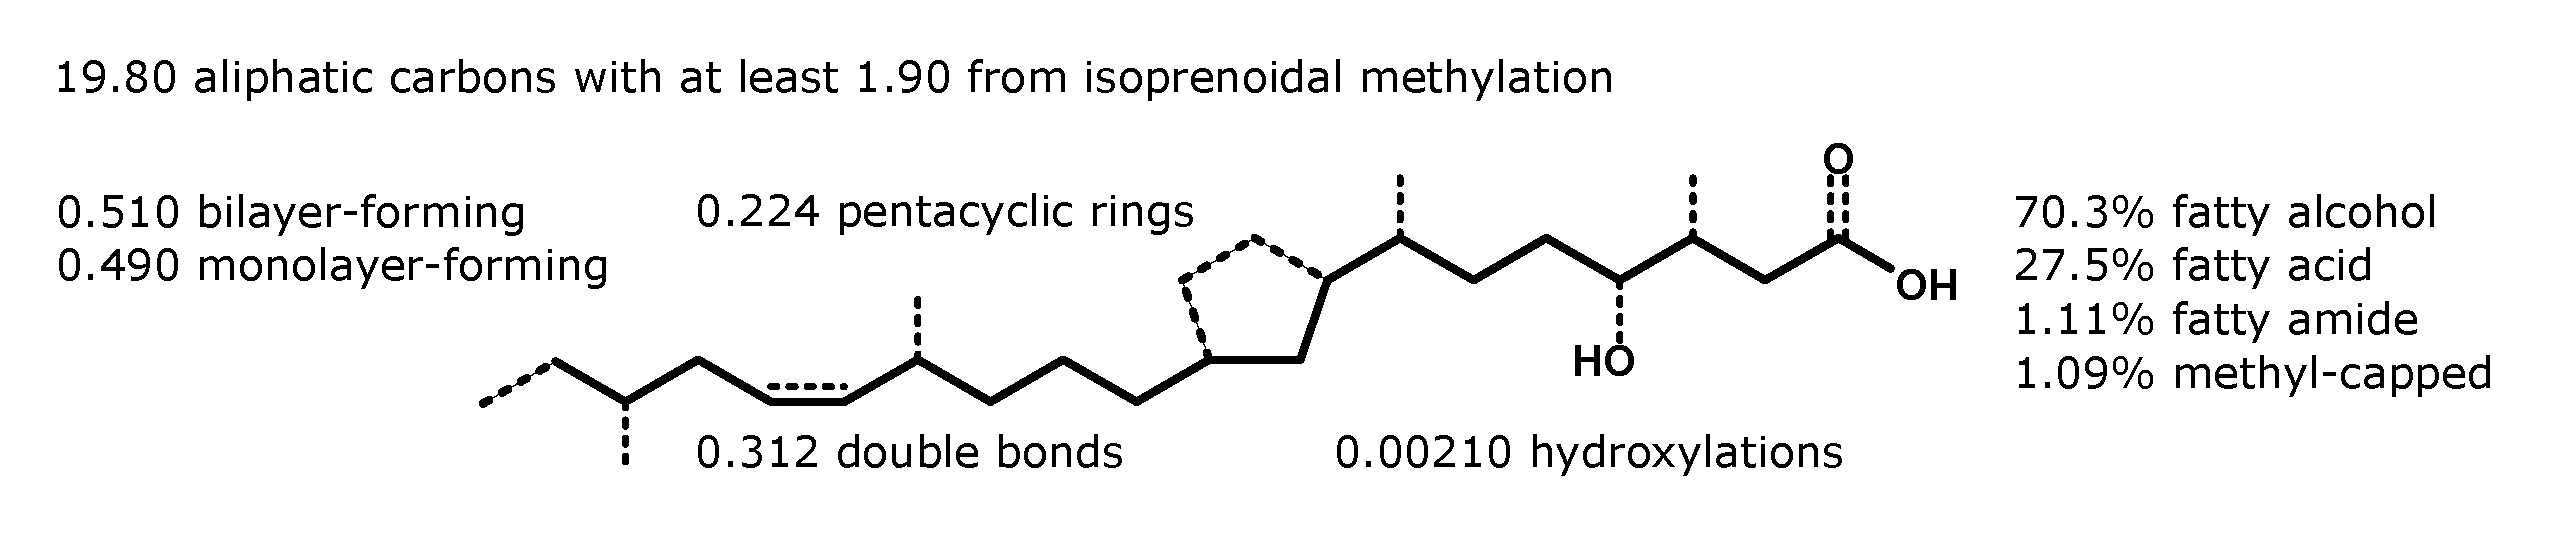
\includegraphics[width=\linewidth]{figs_ch2/sample_average_chain_Bison1}
\caption[Hypothetical chemical structure of the sample-averaged free alkyl chain of Bison Pool sample BP1]{Hypothetical chemical structure of the sample-averaged free alkyl chain (alkyl\textsubscript{free}) of Bison Pool sample BP1 based on abundance-weighted structural characteristics of alkyl chains linked to observed intact polar lipids. Position and isomerism of hydroxylations, pentacyclic rings, methyl branches, and double bonds are not considered when calculating thermodynamic properties of alkyl\textsubscript{free}; their depiction here is to illustrate one of many possible interpretations of a hypothetical average molecule.}
\label{fig:ave_chain}
\end{figure}
\doublespace
\clearpage
}

\afterpage{
\singlespace
\begin{figure}[h]
\centering
\includegraphics[width=\linewidth]{"figs_ch2/linked vs free alkyl chains"}
\caption[Comparison of IPL backbone-alkyl chain linkage types and the free alkyl chains used in thermodynamic calculations]{Comparison of IPL backbone-alkyl chain linkage types (left) and the free alkyl chains used in the thermodynamic calculations of this study (right). R\textsubscript{1} indicates the rest of the alkyl chain and R\textsubscript{2} stands for the remainder of the backbone, headgroup, and other alkyl chains of the IPL. As a part of the thermodynamic estimations performed in this study, abundance-weighted chemical formulae and structures of IPL-linked alkyl chains (orange box, given in Chapter \ref{ch1}) were capped with the elemental and thermodynamic contribution of groups in the yellow box according to alkyl chain-backbone linkage type, arriving at `free' sample-averagedd alkyl chains as a model for sample lipid distributions.}
\label{fig:linked_vs_free_chain}
\end{figure}
\doublespace
\clearpage
}


Various abundance-weighted structural characteristics of alkyl chains such as nC (number of aliphatic carbons), nUnsat (number of unsaturations), nOH (number of secondary hydroxylations), mole fraction of monolayer-forming chains and backbone-chain linkage types (ether, ester, amide, and C-C) were calculated from observed abundances of IPLs reported in Table \ref{tab:mods} of Chapter \ref{ch1}. In this study, partial molal thermodynamic aqueous properties of eighteen hypothetical `sample-averaged' alkyl chains were estimated, each representing the abundance-weighted structural characteristics of alkyl chains in a hot spring sample. For instance, the nC and nUnsat in sample BP1 was observed to be 19.80 and 3.12$\cdot$10\textsuperscript{-1}, respectively, so the thermodynamic properties estimated for the aqueous sample-averaged alkyl chain representing BP1 assume a hypothetical chemical structure with 19.80 aliphatic carbons and 3.12$\cdot$10\textsuperscript{-1} unsaturations, and so on.  A chemical cartoon is shown in Figure \ref{fig:ave_chain} to help visualize what the hypothetical structure of the sample-averaged alkyl chain might look like.

This is equivalent to calculating thermodynamic properties for thousands of individual chains and then taking an abundance-weighted average of each property. It would not have been possible in this study to estimate the thermodynamic properties of every observed chain due to an inability to resolve structural characteristics of individual IPL alkyl chains using this LC-MS method. The rational for calculating thermodynamic properties from abundance-weighted structural characteristics was as follows: if an IPL observed in a sample has 38 aliphatic carbons and two unsaturations distributed between two chains, the structural characteristics of its chains must be described using averages without resorting to assumptions about which chain bears which combination of characteristics, and by extension, the estimated thermodynamic properties of alkyl chains must therefore be described by averages as well. This was taken a step further by assuming that the structural characteristics of all alkyl chains in a sample could be averaged for the sake of calculating thermodynamic properties, resulting the concept of a `sample-averaged' alkyl chain.

In this work, thermodynamic properties were estimated for `free' alkyl chains, as opposed to IPL-linked chains, to provide a simpler model for representing lipid distribution. The difference between IPL-linked and free alkyl chains is represented in Figure \ref{fig:linked_vs_free_chain} for ether-, ester-, amide-, and C-C-linked chains. Except for the C-C linkage type, free chains represent a hydrolyzed version of the IPL-linked chains, with fatty acids, alcohols, and amides corresponding to the free versions of IPL-linked esters, ethers, and amide-bonded alkyl chains. In the case of C-C-linked alkyl chains, the free chain was methyl-capped to maintain alkane-like properties.


A study by \cite{shock1990calculation} demonstrated that the partial molal thermodynamic properties of aqueous hydrocarbons tend to have a strong linear correlation with chain length, as was shown for 1-alkynes, n-alkyl benzenes, 1-alkenes, 1-amines, n-alkanes, aldehydes, 1-alcohols, 2-ketones, methyl alkanoates, n-carboxylic acids, and n-carboxylate ions. This observation served as a theoretical foundation for estimating properties of aqueous alkyl\textsubscript{free} with non-integer values for nC in this work. If a thermodynamic property is linearly correlated with chain length, it should make no difference whether a chain length of 19.0 or 19.8 is used to solve for the value of the property.

\cite{shock1990calculation} also showed that regressed thermodynamic properties with chain length were approximately parallel between different functional group chains and differed only by y-intercept. Because the slopes of these regressions were nearly identical, each additional -CH\textsubscript{2}- group was suggested to contribute the same change in the value of the property. This strongly suggests an additive nature for both functional groups and -CH\textsubscript{2}- in linear organic molecules.

This theory of adding together the contribution of individual chemical groups to arrive at the estimated properties of the entire molecule, or `group additivity', is not new. \cite{sugden1924cxlii} showed that a property related to surface tension, parachor, could be estimated by group additivity for a variety of organic and inorganic compounds, as well as for a few elements. \cite{benson1958additivity} noted that various group additivity rules were cropping up in the literature and proposed a series generalized of rules for estimating thermodynamic properties of ideal gases, including heat capacity, entropy, and heat of formation from the elements. Studies by \cite{cabani1981group, cabani1977volume1, cabani1977volume2} measured volumetric and thermodynamic properties of aqueous molecules and calculated group contribution values of functional groups. Since then, group additivity has been used to estimate the properties of a great many aqueous organic molecules that lack experimentally-measured values.

According to group additivity theory, the thermodynamic contribution of one functional group to molecule is expected to be roughly the same for each addition. This suggests a linear trend in the estimated property as a function of number of times the functional group is added, just as was described above for CH\textsubscript{2} groups. Following the same reasoning that was applied to estimating the properties of a chain with a non-integer nC, we estimated the contributions of non-integer unsaturations, hydroxylations, GDGT cyclic rings, isoprenoidal branching to the thermodynamic properties of alkyl\textsubscript{free}. The fractional contributions of the carboxylic acid, alcohol, methyl-capped, and amide functional group of alkyl\textsubscript{free} were estimated using these guidelines as well.

\section{Methods}
\subsection{Analysis of water chemistry}
Sampling locations were metered and water samples were collected, filtered, and analyzed as described in Chapter \ref{ch1}. Briefly, temperature and pH were metered in the field as close to the sampling locations as possible using a YSI 30 conductivity meter for temperature and a model 3300i or 3110 WTW pH meter with WTW probe for pH. Concentrations of dissolved oxygen and sulfide were measured in unfiltered water samples using Hach 2400 or 2800 portable spectrophotometer with Hach reagents. Water samples collected for laboratory analyses were filtered with Supor (Pall Corporation) filters down to 0.2 microns; samples for ion chromatography were collected in 30 mL HDPE Nalgene bottles (two per sample) and stored at -20$^{\circ}$C before analysis on Dionex DX-600 systems for concentrations of major cations and anions.

Filtered samples for dissolved inorganic carbon (DIC) analysis were collected in acid-washed amber glass vials with black butyl rubber septa. DIC was chemically converted to CO\textsubscript{2} by reacting with phosphoric acid before analysis on an OI Wet Oxidation TOC analyzer coupled to a Thermo Delta Plus Advantage mass spectrometer as described in \cite{havig2011merging}.

The Eh of water samples was calculated using measured concentrations of major dissolved solutes and hot spring temperatures using EQ3/6 aqueous geochemical speciation software version 8.0a \citep{wolery2002eq3} and thermodynamic data from the slop16 database available for download at the URL http://geopig.asu.edu/sites/default/files/slop16.dat

\subsection{Analysis of environmental IPLs} Methods used to collect, identify, and quantify the hot spring microbial IPLs from sediments and biofilms are described in detail in Chapter \ref{ch1}. Briefly, sediments and biofilms were collected into sterile specimen containers with sterilized forceps and spatulas and stored on dry ice the field, and at -80$^{\circ}$C in the lab. Samples were freeze-dried, homogenized with mortar and pestle, and extracted for lipids using a modified version of the Bligh and Dyer method \citep{white1998signature}. Aliquots of the resulting total lipid extracts (TLEs) were analyzed using the hydrophilic interaction chromatography (HILIC) method \citep{wormer2013application} on an Agilent 1200 series high performance liquid chromatograph (HPLC) attached to a Agilent 6520 Accurate-Mass Quadrupole Time-of-Flight Mass Spectrometer with an electrospray ionization source and operated in positive ion mode. Commercially-available standards were used to obtain response factors for calculating IPL mole fractions from mass spectral peak areas. Response factors are given in Table \ref{tab:RF} and assignment to observed IPLs is reported in Table \ref{tab:IPL}.

\subsection{Deriving properties and chemical formulae of alkyl\textsubscript{free}}

\afterpage{
\singlespace
\begin{table}
\centering
% \begin{adjustbox}{width=\textwidth,keepaspectratio}
\begin{threeparttable}
  \caption{Summary of abundance-weighted structural characteristics of isoprenoidal alkyl chains}

% Table generated by Excel2LaTeX from sheet 'leftover isoprenoidal props'
\begin{tabular}{clllcc}
\toprule
Site  & Sample & \multicolumn{1}{c}{$x_{AR}$} & \multicolumn{1}{c}{$x_{GDGT}$} & nPent & nHex \\
\midrule
Bison & BP1   & 1.98$\cdot 10$\textsuperscript{-2} & 4.90$\cdot 10$\textsuperscript{-1} & 2.24$\cdot 10$\textsuperscript{-1} &  \\
Pool  & BP2   & 2.30$\cdot 10$\textsuperscript{-2} & 3.00$\cdot 10$\textsuperscript{-1} & 1.63$\cdot 10$\textsuperscript{-1} &  \\
      & BP3   & 1.49$\cdot 10$\textsuperscript{-3} & 8.81$\cdot 10$\textsuperscript{-2} & 6.19$\cdot 10$\textsuperscript{-2} &  \\
      & BP4   &       & 7.16$\cdot 10$\textsuperscript{-3} & 5.52$\cdot 10$\textsuperscript{-3} &  \\
      & BP5   & 5.06$\cdot 10$\textsuperscript{-6} & 7.20$\cdot 10$\textsuperscript{-4} & 5.69$\cdot 10$\textsuperscript{-4} &  \\
      & BP6   &       & 2.94$\cdot 10$\textsuperscript{-3} & 2.40$\cdot 10$\textsuperscript{-3} &  \\
      &       &       &       &       &  \\
Mound & MS1   &       & 9.99$\cdot 10$\textsuperscript{-1} & 6.16$\cdot 10$\textsuperscript{-1} & 2.68$\cdot 10$\textsuperscript{-3} \\
Spring & MS2   & 2.30$\cdot 10$\textsuperscript{-2} & 6.07$\cdot 10$\textsuperscript{-1} & 3.01$\cdot 10$\textsuperscript{-1} &  \\
      & MS3   &       & 1.64$\cdot 10$\textsuperscript{-1} & 1.13$\cdot 10$\textsuperscript{-1} &  \\
      & MS4   &       & 5.85$\cdot 10$\textsuperscript{-2} & 4.25$\cdot 10$\textsuperscript{-2} &  \\
      & MS5   &       & 1.09$\cdot 10$\textsuperscript{-2} & 9.65$\cdot 10$\textsuperscript{-3} &  \\
      &       &       &       &       &  \\
Empress & EP1   & 1.97$\cdot 10$\textsuperscript{-2} & 8.63$\cdot 10$\textsuperscript{-1} & 4.45$\cdot 10$\textsuperscript{-1} & 1.09$\cdot 10$\textsuperscript{-2} \\
Pool  & EP2   & 4.74$\cdot 10$\textsuperscript{-3} & 4.71$\cdot 10$\textsuperscript{-1} & 2.91$\cdot 10$\textsuperscript{-1} & 7.83$\cdot 10$\textsuperscript{-3} \\
      & EP3   & 2.21$\cdot 10$\textsuperscript{-3} & 6.06$\cdot 10$\textsuperscript{-1} & 3.61$\cdot 10$\textsuperscript{-1} & 1.15$\cdot 10$\textsuperscript{-2} \\
      & EP4   & 4.08$\cdot 10$\textsuperscript{-3} & 2.31$\cdot 10$\textsuperscript{-1} & 1.43$\cdot 10$\textsuperscript{-1} & 2.98$\cdot 10$\textsuperscript{-3} \\
      & EP5   & 2.78$\cdot 10$\textsuperscript{-3} & 1.26$\cdot 10$\textsuperscript{-1} & 7.19$\cdot 10$\textsuperscript{-2} & 1.12$\cdot 10$\textsuperscript{-3} \\
      &       &       &       &       &  \\
Octopus & OS1   & 1.26$\cdot 10$\textsuperscript{-1} & 4.21$\cdot 10$\textsuperscript{-1} & 1.20$\cdot 10$\textsuperscript{-1} &  \\
Spring & OS2   & 5.08$\cdot 10$\textsuperscript{-6} & 7.60$\cdot 10$\textsuperscript{-3} & 4.21$\cdot 10$\textsuperscript{-3} & 1.46$\cdot 10$\textsuperscript{-4} \\
\bottomrule
\end{tabular}%
  
  \begin{tablenotes}
    % The order of footnotes here will determine their letter in the table
    \item
        
  \end{tablenotes}
  
  \label{tab:leftover_props}
  \end{threeparttable}
%   \end{adjustbox}
\end{table}
\setcounter{tabcounter}{0} % reset custom table footnote counter
\doublespace
\clearpage
}

Calculation of the elemental abundance of alkyl\textsubscript{free} began with the chemical formulae of sample-averaged IPL-linked alkyl chains, to which additional carbon, hydrogen, oxygen, and nitrogen were added to convert ether-linked chains into free fatty alcohols, ester-linked chains into free fatty acids, amide-linked chains into free fatty amides, and C-C-linked chains into free methyl-capped chains. Chemical formulae of sample-averaged IPL-linked alkyl chains and mole fractions of alkyl chain linkage types required for these calculations are reported in Table \ref{tab:leftover_props} for isoprenoidal chains and Table \ref{tab:mods} in Chapter \ref{ch1} for all others.

The number of carbon atoms ($c_{free}$) in the chemical formulae of alkyl\textsubscript{free} was calculated with

\begin{equation}
    c_{free} = c_{linked} + x_{cc}
\end{equation}

\noindent where $c_{linked}$ indicates the number of carbon atoms in the sample-averaged IPL-linked alkyl chain of the sample, and $x_{cc}$ stands for the observed mole fraction of C-C-linked alkyl chains. Addition of a number of carbons equal to $x_{cc}$ to $c_{linked}$ accounts for the carbon that would be gained with a terminal methyl group assuming hypothetical carbon-carbon bond breakage of C-C-linked alkyl chains to produce the sample-averaged free chains considered in this study.

The number of hydrogen atoms ($h_{free}$) in the chemical formulae of alkyl\textsubscript{free} was calculated with

\begin{align}
\begin{split}
    h_{free} = &h_{linked} + x_{ether} + x_{ester}\\
        & + 2(x_{amide}) + 3(x_{cc}) \\
\end{split}
\end{align}

\noindent where $h_{linked}$ represents the number of hydrogen atoms in the sample-averaged IPL-linked alkyl chain of the sample, and $x_{ether}$, $x_{ester}$, and $x_{amide}$ correspond to the observed mole fractions of ether-, ester-, and amide-linked alkyl chains, respectively. A number of hydrogens equal to $x_{ether}$ and $x_{ester}$ are added to $h_{linked}$ to account for the single hydrogen in the hydroxyl groups of the resulting alcohol and carboxylic acid group assuming hypothetical hydrolysis of ether- and ester-linked chains to produce free fatty acids and fatty alcohols. Similarly, two times $x_{amide}$ is added to account for the two hydrogen atoms in the amine group of the free amide after the hypothetical hydrolysis of an amide-linked chain. Lastly, adding a number of hydrogens equal to three times $x_{cc}$ accounts for the three hydrogen atoms added by a terminal methyl group after the hypothetical carbon-carbon breakage of a C-C-linked alkyl chain.

The number of nitrogen atoms ($n_{free}$) in the chemical formulae of alkyl\textsubscript{free} was calculated with

\begin{equation}
    n_{free} = n_{linked} + x_{amide}
\end{equation}

\noindent where $n_{linked}$ indicates the number of nitrogen atoms in the sample-averaged IPL-linked alkyl chain. A number of nitrogen atoms equal to $x_{amide}$ is added to $n_{linked}$ to account for the single nitrogen atom added by the amine group of the free amide after hypothetical hydrolysis of an amide-linked alkyl chain.

The number of oxygen atoms ($o_{free}$) in the chemical formulae of alkyl\textsubscript{free} was calculated with

\begin{equation}
    o_{free} = o_{linked} + x_{ether} + x_{ester}
\end{equation}

\noindent where $o_{linked}$ is the number of oxygen atoms in the sample-averaged IPL-linked alkyl chain. A number of oxygen atoms equal to $x_{ether}$ and $x_{ester}$ are added to $o_{linked}$ to account for the single oxygen atom in the hydroxyl groups of the resulting alcohol and carboxylic acid group assuming hypothetical hydrolysis of ether- and ester-linked chains to produce free fatty acids and fatty alcohols.

\subsection{Calculation of thermodynamic properties}

\afterpage{
\singlespace
\begin{table}
\centering
\begin{adjustbox}{height=\textheight,keepaspectratio}
\begin{threeparttable}
  \caption{Partial molal thermodynamic aqueous and hydration properties of aliphatic carboxylic acids, alcohols, and alkanes with nC $>$ 2 used in the estimation of saturated fatty acid, fatty alcohol, and fatty hydrocarbon properties.}



% Table generated by Excel2LaTeX from sheet 'linkage thermo table'
\begin{tabular}{lrrrrr}
\toprule
      & $\Delta_{f}G^{\circ}_{aq}$\rtr{linkage_kjpermol} & $\Delta_{f}H^{\circ}_{aq}$\rtr{linkage_kjpermol} & $Cp^{\circ}_{aq}$\rtr{linkage_jpermolk} & $V^{\circ}_{aq}$\rtr{linkage_cm3permol} & $\Delta_{h}G^{\circ}$\rtr{linkage_kjpermol} \\
\midrule
propanoic acid & -390.99 & -512.41 & 253   & 67.9  & -21.4\rtr{khan1992henry} \\
n-butanoic acid & -381.62 & -535.34 & 337   & 84.61 & -20.9\rtr{khan1992henry} \\
n-pentanoic acid & -373.38 & -559.36 & 432.2 & 100.5 & -19.0\rtr{khan1992henry} \\
n-hexanoic acid & -364.51 & -582.79 & 523.0 & 116.55 & -17.8\rtr{khan1992henry} \\
n-heptanoic acid & -356.48 & -607.01 & 611.7 & 131.6 &  \\
n-octanoic acid & -349.15 & -631.99 & 700.4 & 147.4 &  \\
n-nonanoic acid & -339.82 & -654.92 & 789.1 & 163.2 &  \\
n-decanoic acid & -331.25 & -678.64 & 877.8 & 179.0 &  \\
n-undecanoic acid & -322.71 & -702.37 & 966.5 & 194.8 &  \\
n-dodecanoic acid & -314.13 & -726.09 & 1055  & 210.6 &  \\
1-propanol & -172.07 & -312.74 & 355   & 70.71 & -12.36 \\
1-butanol & -162.40 & -336.53 & 443   & 86.53 & -11.86 \\
1-pentanol & -151.72 & -359.56 & 535   & 102.50 & -11.11 \\
1-hexanol & -143.31 & -383.79 & 617   & 118.46 & -10.30 \\
1-heptanol & -134.41 & -408.39 & 702   & 133.03 & -9.72 \\
1-octanol & -123.93 & -429.85 & 778   & 151.20 & -9.14 \\
1-nonanol & -115.24 & -454.67 & 865   & 164.55 & -8.36 \\
1-decanol & -106.23 & -478.75 & 950   & 180.16 & -8.18 \\
1-undecanol & -96.52 & -502.77 & 1034  & 195.77 & -6.90 \\
1-dodecanol & -86.17 & -525.73 & 1119  & 211.38 & -6.04 \\
propane & -8.22 & -127.43 & 398   & 69.31 & 16.09 \\
n-butane & 0.24  & -151.53 & 482   & 75.55 & 16.58 \\
n-pentane & 8.88  & -175.45 & 573   & 99.07 & 17.52 \\
n-hexane & 19.26 & -198.69 & 636   & 114.68 & 18.26 \\
n-heptane & 27.45 & -224.54 & 739   & 130.29 & 18.95 \\
n-octane & 36.08 & -250.45 & 824   & 145.90 & 19.64 \\
n-nonane & 46.24 & -275.24 & 908   & 161.51 & 20.51 \\
n-decane & 55.50 & -296.34 & 993   & 177.12 & 21.24 \\
n-undecane & 64.71 & -321.12 & 1078  & 192.73 & 22.94 \\
n-dodecane & 74.65 & -343.26 & 1163  & 208.34 & 22.51 \\
n-tridecane & 81.58 & -368.84 & 1248  & 223.95 & 22.87 \\
n-tetradecane & 90.85 & -392.99 & 1333  & 239.56 & 23.55 \\
\bottomrule
\end{tabular}%


  
  \begin{tablenotes}
    % The order of footnotes here will determine their letter in the table
    Carboxylic acid properties are taken from \cite{shock1995organic} unless otherwise noted. Properties for alcohols and alkanes are recommended values from the ORganic Compounds HYDration properties (ORCHYD) database compiled by \cite{plyasunova2004database}.
    
    \tr{linkage_kjpermol} kJ mol\textsuperscript{-1},
    \tr{linkage_jpermolk} J mol\textsuperscript{-1} K\textsuperscript{-1},
    \tr{linkage_cm3permol} cm\textsuperscript{3} mol\textsuperscript{-1},
    \tr{khan1992henry} values calculated from Henry's law constants, $K_{H}$, reported in \cite{khan1992henry} using the relation $\Delta_{h}G^{\circ} = -RT\ln{K_{H}}$.
        
  \end{tablenotes}
  
  \label{tab:carbacid_alc_alk_props}
  \end{threeparttable}
  \end{adjustbox}
\end{table}
\setcounter{tabcounter}{0} % reset custom table footnote counter
\doublespace
\clearpage
}


\afterpage{
\singlespace
\begin{table}
\centering
\begin{threeparttable}
  \caption{Regressed partial molal properties of fatty acids, fatty alcohols, and alkanes with nC $>$ 2 as a function of chain length.}


% Table generated by Excel2LaTeX from sheet 'linkage regress table'
\begin{tabular}{llrrrr}
\toprule
property & chain type & slope & intercept & R\textsuperscript{2} & p-value\rtr{regress_pval} \\
\midrule
$\Delta_{f}G^{\circ}_{aq}$\rtr{linkage_kjpermol} & fatty acid & 8.46  & -415.87 & $>$0.99 & 2.50E-15 \\
      & fatty alcohol & 9.43  & -199.95 & $>$0.99 & 5.40E-15 \\
      & alkane & 9.10  & -35.95 & $>$0.99 & 4.10E-18 \\
\midrule
$\Delta_{f}H^{\circ}_{aq}$\rtr{linkage_kjpermol} & fatty acid & -23.82 & -440.45 & $>$0.99 & 6.30E-19 \\
      & fatty alcohol & -23.70 & -241.52 & $>$0.99 & 6.50E-18 \\
      & alkane & -24.14 & -55.30 & $>$0.99 & 9.40E-20 \\
\midrule
$Cp^{\circ}_{aq}$\rtr{linkage_jpermolk} & fatty acid & 89    & -15   & $>$0.99 & 3.30E-18 \\
      & fatty alcohol & 84    & 108   & $>$0.99 & 4.60E-16 \\
      & alkane & 85    & 140   & $>$0.99 & 5.10E-19 \\
\midrule
$V^{\circ}_{aq}$\rtr{linkage_cm3permol} & fatty acid & 15.8  & 21.3  & $>$0.99 & 2.00E-18 \\
      & fatty alcohol & 15.61 & 24.36 & $>$0.99 & 1.10E-15 \\
      & alkane & 15.80 & 18.84 & $>$0.99 & 2.30E-15 \\
\midrule
$\Delta_{h}G^{\circ}$\rtr{linkage_kjpermol} & fatty acid & 1.3   & -25.5 & 0.96  & 0.021 \\
      & fatty alcohol & 0.68  & -14.52 & 0.99  & 2.30E-09 \\
      & alkane & 0.72  & 13.97 & 0.98  & 1.30E-09 \\
\bottomrule
\end{tabular}%

  
  \begin{tablenotes}
    % The order of footnotes here will determine their letter in the table
    Regressed thermodynamic properties are given in Table \ref{tab:carbacid_alc_alk_props}.
    
    \tr{regress_pval} F-test p-value for linear model,
    \tr{grpadd_chain_kjpermol} kJ mol\textsuperscript{-1},
    \tr{grpadd_chain_jpermolk} J mol\textsuperscript{-1} K\textsuperscript{-1},
    \tr{grpadd_chain_cm3permol} cm\textsuperscript{3} mol\textsuperscript{-1}
    
        
  \end{tablenotes}
  
  \label{tab:regress_chain_prop}
  \end{threeparttable}
\end{table}
\setcounter{tabcounter}{0} % reset custom table footnote counter
\doublespace
\clearpage
}



Thermodynamic properties for alkyl\textsubscript{free} were estimated assuming the species were in the aqueous phase. The standard state convention for species in the aqueous phase assumed unit activity in a hypothetical 1 mol$\cdot$kg$^{-1}$ solution referenced to infinite dilution at any temperature and pressure. The standard state used for liquid water was one unit activity of pure H$_{2}$O at any temperature and pressure. The standard state used for gaseous species was unit fugacity of the ideal gas at 1 bar and any temperature. Hydration properties were chosen to reflect the equilibrium process of transferring 1 mole of the species in the gas phase to the aqueous phase \citep{plyasunov2000thermodynamic}.

Aqueous partial molal thermodynamic Gibbs free energies and enthalpies of formation from the elements ($\Delta_{f}G_{aq}^{\circ}$ and $\Delta_{f}H_{aq}^{\circ}$, respectively), volumes ($V_{aq}^{\circ}$), heat capacities ($Cp_{aq}^{\circ}$), and Gibbs free energies of the hydration process ($\Delta_{h}G^{\circ}$) were estimated for alkyl\textsubscript{free} in two steps. The goal of the first step was to estimate the properties of a saturated, straight aliphatic chain of length of nC and terminating at one end with a hybrid functional group. This hybrid group was a combination of alcohol, carboxylic acid, alkane, and amide, with the fraction of each set by observed mole fractions of ether, ester, C-C, and amide-linked IPL alkyl chains, respectively. 

Experimentally-derived thermodynamic properties for n-carboxylic acids, 1-alcohols, and alkanes were gathered from the literature into Table \ref{tab:carbacid_alc_alk_props} and then regressed as a linear function of chain length. The results of these regressions are shown in Table \ref{tab:regress_chain_prop}. Properties for n-amides were not readily available, and were estimated using a different method, described later.
The slopes and intercepts of these regressions were used to estimate the properties of a hybrid fatty alkyl chain, $\Xi_{fatty}$, in the equation

\begin{align}
\begin{split}
\Xi_{fatty} = & (m_{alcohol}\cdot \text{nC} + b_{alcohol})(x_{ether}) \\
            + & (m_{acid}\cdot \text{nC} + b_{acid})(x_{ester}) \\
            + & (m_{alkane}\cdot \text{nC} + b_{alkane})(x_{cc}) \\
            + & (m_{acid}\cdot \text{nC} + b_{acid} + \Delta\Xi_{amide})(x_{amide}) \\
\end{split}
\end{align}

\noindent where $m_{alcohol}$, $m_{acid}$, $m_{alkane}$, $b_{alcohol}$, $b_{acid}$, $b_{alkane}$ correspond to the slopes ($m$) and intercepts ($b$) of linear regressions of the value of each thermodynamic property as a function of chain length for fatty acids, fatty alcohols, and alkanes. $x_{ether}$, $x_{ester}$, $x_{cc}$, and $x_{amide}$ represent the mole fractions of ether-linked, ester-linked, C-C-linked, amide-linked, and GDGT alkyl chains observed in the sample, respectively. $\Delta\Xi_{amide}$ indicates the estimated difference in the thermodynamic property between a fatty amid and fatty acid, which is given in Table \ref{tab:amide}. The first three terms of this equation use the slopes and intercepts of the regression of the property of interest to obtain the property of a straight fatty chain with a length equal to nC, and then weights the contributions of those properties by the mole fractions of observed IPL alkyl chain linkages; fatty alcohols, fatty acids, and fatty alkanes by the mole fractions of ethers, esters, and C-C linked alkyl chains, respectively. In the fourth term of the equation, a carboxylic acid of length nC was instead estimated by $m_{acid}\cdot \text{nC} + b_{acid}$, to which $\Delta\Xi_{amide}$ was added to convert the carboxylic acid into an amide. The contribution of fatty amides to $\Xi_{fatty}$ was not estimated by regression of aqueous amide properties in the same way as alcohols, carboxylic acids, and alkanes due to a lack of literature data, necessitating the carboxylic acid to amide correction, $\Delta\Xi_{amide}$.


\afterpage{
\singlespace
\begin{table}
\centering
% \begin{adjustbox}{width=\textheight,keepaspectratio}
\begin{threeparttable}
  \caption{Partial molal thermodynamic aqueous and hydration properties of functional groups and chemical species used in the estimation of fatty amide properties.}



% Table generated by Excel2LaTeX from sheet 'fatty amide table'
\begin{tabular}{lrrrrr}
\toprule
      & $\Delta_{f}G^{\circ}_{aq}$\rtr{linkage_kjpermol} & $\Delta_{f}H^{\circ}_{aq}$\rtr{linkage_kjpermol} & $Cp^{\circ}_{aq}$\rtr{linkage_jpermolk} & $V^{\circ}_{aq}$\rtr{linkage_cm3permol} & $\Delta_{h}G^{\circ}$\rtr{linkage_kjpermol} \\
\midrule
$\lbrack$-CONH\textsubscript{2}$\rbrack$ & -194.8\rtr{amide_dick2006temperature} & -257.0\rtr{amide_dick2006temperature} & 21\rtr{amide_dick2006temperature} & 28.2\rtr{amide_dick2006temperature} &  \\
$\lbrack$-COOH$\rbrack$ & -387.3\rtr{amide_dick2006temperature} & -436.7\rtr{amide_dick2006temperature} & 22\rtr{amide_dick2006temperature} & 24.5\rtr{amide_dick2006temperature} &  \\
acetamide &       &       &       &       & -32.7\rtr{amide_sedlbauer2012database} \\
acetic acid &       &       &       &       & -21.0\rtr{amide_khan1992henry} \\
\midrule
$\Delta\Xi_{amide}$ & 192.5\rtr{amide_groupsubtract} & 179.7\rtr{amide_groupsubtract} & -1\rtr{amide_groupsubtract} & 3.7\rtr{amide_groupsubtract} & -11.7\rtr{amide_acetamidesubtract} \\
\bottomrule
\end{tabular}%
  
  \begin{tablenotes}
    % The order of footnotes here will determine their letter in the table

    \tr{amide_kjpermol} kJ mol\textsuperscript{-1},
    \tr{amide_jpermolk} J mol\textsuperscript{-1} K\textsuperscript{-1},
    \tr{amide_cm3permol} cm\textsuperscript{3} mol\textsuperscript{-1},
    \tr{amide_dick2006temperature} \cite{dick2006temperature},
    \tr{amide_sedlbauer2012database} value from \cite{cabani1981group} with an adjustment of +7.9 kJ/mol to convert the standard state definition used by the authors for gases (1M ideal gas) to those used here (pure ideal gas) when deriving properties of the hydration process, as reported in the \textit{Database on the infinite dilution  partial  molar Gibbs  energies of hydration of aqueous organic nonelectrolytes} \citep{sedlbauer2012database, sedlbauer2002group},
    \tr{amide_khan1992henry} values calculated from Henry's law constants, $K_{H}$, reported in \cite{khan1992henry} using the relation $\Delta_{h}G^{\circ} = -RT\ln{K_{H}}$,
    \tr{amide_groupsubtract} estimated from $\Xi_{[-CONH_{2}]} - \Xi_{[-COOH]}$, where $\Xi_{[-CONH_{2}]}$ and $\Xi_{[-COOH]}$ are the properties of [-CONH\textsubscript{2}] and [-COOH] given in the table, respectively,
    \tr{amide_acetamidesubtract} estimated from $\Xi_{acetamide} - \Xi_{acetate}$, where $\Xi_{acetamide}$ and $\Xi_{acetate}$ are the properties of acetamide and acetate given in the table, respectively.
    
        
  \end{tablenotes}
  
  \label{tab:amide}
  \end{threeparttable}
 % \end{adjustbox}
\end{table}
\setcounter{tabcounter}{0} % reset custom table footnote counter
\doublespace
\clearpage
}


\afterpage{
\singlespace
\begin{table}
% \begin{adjustbox}{width=\linewidth,keepaspectratio}
\centering
\begin{threeparttable}
  \caption{Partial molal thermodynamic data for alkenes used in the estimation of unsaturated alkyl chain properties.}


% Table generated by Excel2LaTeX from sheet 'Thermo unsat'
\begin{tabular}{lrrrrr}
\toprule
      & $\Delta_{f}G^{\circ}_{aq}$\rtr{unsat_kjpermol} & $\Delta_{f}H^{\circ}_{aq}$\rtr{unsat_kjpermol} & $Cp^{\circ}_{aq}$\rtr{unsat_jpermolk} & $V^{\circ}_{aq}$\rtr{unsat_cm3permol} & $\Delta_{h}G^{\circ}$\rtr{unsat_kjpermol} \\
\midrule
2-pentene & 83.09 & -59.2 & 535   & 87.00 & 13.44 \\
2-heptene & 99.65 & -109.3 & 709   & 118.40 & 14.77 \\
\midrule
$\Delta\Xi_{unsat}$ & 73.205\rtr{add_unsat} & 115.7\rtr{add_unsat} & -34\rtr{add_unsat} & -11.98\rtr{add_unsat} & -4.13\rtr{add_unsat} \\
\bottomrule
\end{tabular}%



  
  \begin{tablenotes}
    % The order of footnotes here will determine their letter in the table
    Properties in this table are recommended values from the ORganic Compounds HYDration properties (ORCHYD) database compiled by \cite{plyasunova2004database} unless otherwise noted.
    
    \tr{unsat_kjpermol} kJ mol\textsuperscript{-1},
    \tr{unsat_jpermolk} J mol\textsuperscript{-1} K\textsuperscript{-1},
    \tr{unsat_cm3permol} cm\textsuperscript{3} mol\textsuperscript{-1},
    \tr{add_unsat} estimated by taking the average of $\Xi_{2-pentene} - \Xi_{pentane}$ and $\Xi_{2-heptene} - \Xi_{heptane}$, where $\Xi_{2-pentene}$, and $\Xi_{2-heptene}$ are the properties of 2-pentane and 2-heptene given in the table and $\Xi_{pentane}$, and $\Xi_{heptane}$ are the properties of pentane and heptane given in Table \ref{tab:carbacid_alc_alk_props}.
    
        
  \end{tablenotes}
  
  \label{tab:unsat}
  \end{threeparttable}
%   \end{adjustbox}
\end{table}
\setcounter{tabcounter}{0} % reset custom table footnote counter
\doublespace
\clearpage
}


\afterpage{
\begin{landscape}
\singlespace
\begin{table}
\centering
\begin{adjustbox}{width=600pt,keepaspectratio}
\begin{threeparttable}
  \caption{Partial molal thermodynamic data for second order groups used in the estimation of alkyl chain methyl branching, hydroxylation, and monolayer-spanning characteristics.}


% Table generated by Excel2LaTeX from sheet 'Thermo 2nd Order'
\begin{tabular}{llrrrrrrrrrrrr}
\toprule
Group & Formula & $\Delta_{f}G^{\circ}_{aq}$\rtr{grpadd_chain_kjpermol} & $\Delta_{f}H^{\circ}_{aq}$\rtr{grpadd_chain_kjpermol} & $S^{\circ}_{aq}$\rtr{grpadd_chain_jpermolk} & $Cp^{\circ}_{aq}$\rtr{grpadd_chain_jpermolk} & $V^{\circ}_{aq}$\rtr{grpadd_chain_cm3permol} & $\Delta_{h}G^{\circ}$\rtr{grpadd_chain_kjpermol} & $\Delta_{h}H^{\circ}$\rtr{grpadd_chain_kjpermol} & $\Delta_{h}S^{\circ}$\rtr{grpadd_chain_jpermolk} & $\Delta_{h}Cp^{\circ}$\rtr{grpadd_chain_jpermolk} & $\Delta_{f}H^{\circ}_{ig}$\rtr{grpadd_chain_kjpermol} & $S^{\circ}_{ig}$\rtr{grpadd_chain_jpermolk} & $Cp^{\circ}_{ig}$\rtr{grpadd_chain_jpermolk} \\
\midrule
C-(H)\textsubscript{2}(C)\textsubscript{2} & CH\textsubscript{2} & 9.05\rtr{grpadd_chain_GHS} & -24.15\rtr{grpadd_chain_HaqHhHig} & 25.07\rtr{grpadd_chain_SaqShSig} & 85\rtr{grpadd_chain_CpaqCphCpig} & 15.61\rtr{plyasunov2004group} & 0.68\rtr{plyasunov2004group} & -3.52\rtr{plyasunov2004group} & -14.09\rtr{grpadd_chain_GhHhSs} & 62\rtr{plyasunov2004group} & -20.63\rtr{domalski1993estimation} & 39.16\rtr{domalski1993estimation} & 22.89\rtr{domalski1993estimation} \\
C-(H)(C)\textsubscript{3} & CH    & 34.07\rtr{grpadd_chain_GHS} & 1.17\rtr{grpadd_chain_HaqHhHig} & -39.28\rtr{grpadd_chain_SaqShSig} & 3\rtr{grpadd_chain_CpaqCphCpig} & 5.96\rtr{plyasunov2004group} & -1.93\rtr{plyasunov2004group} & 2.34\rtr{plyasunov2004group} & 14.32\rtr{grpadd_chain_GhHhSs} & -17\rtr{plyasunov2004group} & -1.17\rtr{domalski1993estimation} & -53.60\rtr{domalski1993estimation} & 20.08\rtr{domalski1993estimation} \\
C-(H)\textsubscript{3}(C) & CH\textsubscript{3} & -16.35\rtr{grpadd_chain_GHS} & -50.45\rtr{grpadd_chain_HaqHhHig} & 87.37\rtr{grpadd_chain_SaqShSig} & 158\rtr{grpadd_chain_CpaqCphCpig} & 25.56\rtr{plyasunov2004group} & 3.72\rtr{plyasunov2004group} & -8.19\rtr{plyasunov2004group} & -39.95\rtr{grpadd_chain_GhHhSs} & 132\rtr{plyasunov2004group} & -42.26\rtr{domalski1993estimation} & 127.32\rtr{domalski1993estimation} & 25.73\rtr{domalski1993estimation} \\
C-(H)(O)(C)\textsubscript{2} & CH    & 6.29\rtr{grpadd_chain_GHS} & -27.98\rtr{grpadd_chain_HaqHhHig} & -43.85\rtr{grpadd_chain_SaqShSig} & 26\rtr{grpadd_chain_CpaqCphCpig} & 7.48\rtr{plyasunov2004group} & -1.64\rtr{plyasunov2004group} & -1.88\rtr{plyasunov2004group} & -0.80\rtr{grpadd_chain_GhHhSs} & 6\rtr{plyasunov2004group} & -26.10\rtr{domalski1993estimation} & -43.05\rtr{domalski1993estimation} & 19.96\rtr{domalski1993estimation} \\
O-(H)(C) & OH    & -170.59\rtr{grpadd_chain_GHS} & -197.67\rtr{grpadd_chain_HaqHhHig} & 78.30\rtr{grpadd_chain_SaqShSig} & 27\rtr{grpadd_chain_CpaqCphCpig} & 11.35\rtr{plyasunov2004group} & -25.46\rtr{plyasunov2004group} & -38.34\rtr{plyasunov2004group} & -43.20\rtr{grpadd_chain_GhHhSs} & 9\rtr{plyasunov2004group} & -159.33\rtr{domalski1993estimation} & 121.5\rtr{domalski1993estimation} & 18.16\rtr{domalski1993estimation} \\
\midrule
$\Delta\Xi_{methyl}$ & 2$\times$CH\textsubscript{2}$\rightarrow$CH(CH3) & 0.38\rtr{add_branching} & -0.98\rtr{add_branching} &       & 9\rtr{add_branching} & 0.30\rtr{add_branching} & 0.43\rtr{add_branching} &       &       &       &       &       &  \\
$\Delta\Xi_{hydroxyl}$ & CH\textsubscript{2}$\rightarrow$CH(OH) & -173.35\rtr{add_hydroxyl} & -201.50\rtr{add_hydroxyl} &       & -32\rtr{add_hydroxyl} & 3.22\rtr{add_hydroxyl} & -27.78\rtr{add_hydroxyl} &       &       &       &       &       &  \\
$\Delta\Xi_{monolayer}$ & CH\textsubscript{3}$\rightarrow$CH\textsubscript{2} & 25.40\rtr{add_CH2} & 26.30\rtr{add_CH2} &       & -73\rtr{add_CH2} & 9.65\rtr{add_CH2} & -3.04\rtr{add_CH2} &       &       &       &       &       &  \\
\bottomrule
\end{tabular}%

  
  \begin{tablenotes}
    % The order of footnotes here will determine their letter in the table
    \tr{grpadd_chain_kjpermol} kJ mol\textsuperscript{-1},
    \tr{grpadd_chain_jpermolk} J mol\textsuperscript{-1} K\textsuperscript{-1},
    \tr{grpadd_chain_cm3permol} cm\textsuperscript{3} mol\textsuperscript{-1},
    \tr{grpadd_chain_GHS} calculated using $\Delta_{f}H^{\circ}_{aq}$ and $S^{\circ}_{aq}$ given in the table along with $S^{\circ}$ of the elements referenced from \cite{cox1989codata} and the relation $\Delta_{f}G^{\circ}_{aq} = \Delta_{f}H^{\circ}_{aq} - T\Delta(S_{aq}^{\circ}-\sum S_{elements}^{\circ}$),
    \tr{grpadd_chain_HaqHhHig} calculated using $\Delta_{h}H^{\circ}$ and $\Delta_{f}H^{\circ}_{ig}$ given in the table and the relation $\Delta_{f}H^{\circ}_{aq} = \Delta_{h}H^{\circ} + \Delta_{f}H^{\circ}_{ig}$,
    \tr{grpadd_chain_SaqShSig} calculated using $\Delta_{h}S^{\circ}$ and $S^{\circ}_{ig}$ given in the table and the relation $S^{\circ}_{aq} = \Delta_{h}S^{\circ} + S^{\circ}_{ig}$,
    \tr{grpadd_chain_CpaqCphCpig} calculated using $\Delta_{h}Cp^{\circ}$ and $Cp^{\circ}_{ig}$ given in the table and the relation $Cp^{\circ}_{aq} = \Delta_{h}Cp^{\circ} + Cp^{\circ}_{ig}$,
    \tr{plyasunov2004group} \cite{plyasunov2004group},
    \tr{grpadd_chain_GhHhSs} calculated using $\Delta_{h}G^{\circ}$ and $\Delta_{h}H^{\circ}$ given in the table and the relation $\Delta_{h}G^{\circ} = \Delta_{h}H^{\circ} - T\Delta_{h} S^{\circ}$,
    \tr{domalski1993estimation} \cite{domalski1993estimation},
    \tr{add_branching} estimated from $\Xi_{C-(H)(C)\textsubscript{3}} + \Xi_{C-(H)\textsubscript{3}(C)} - 2\times\Xi_{C-(H)\textsubscript{2}(C)\textsubscript{2}}$, where $\Xi_{C-(H)(C)\textsubscript{3}}$, $\Xi_{C-(H)\textsubscript{3}(C)}$, and $\Xi_{C-(H)\textsubscript{2}(C)\textsubscript{2}}$ are the properties of C-(H)(C)\textsubscript{3}, C-(H)\textsubscript{3}(C), and C-(H)\textsubscript{2}(C)\textsubscript{2} given in the table, respectively,
    \tr{add_hydroxyl} estimated from $\Xi_{C-(H)(O)(C)\textsubscript{2}} + \Xi_{O-(H)(C)} - \Xi_{C-(H)\textsubscript{2}(C)\textsubscript{2}}$, where $\Xi_{C-(H)(O)(C)\textsubscript{2}}$, $\Xi_{O-(H)(C)}$, and $\Xi_{C-(H)\textsubscript{2}(C)\textsubscript{2}}$ are the properties of C-(H)(O)(C)\textsubscript{2}, O-(H)(C), and C-(H)\textsubscript{2}(C)\textsubscript{2} given in the table, respectively,
    \tr{add_CH2}  estimated from $\Xi_{C-(H)\textsubscript{3}(C)} - \Xi_{C-(H)\textsubscript{2}(C)\textsubscript{2}}$, where $\Xi_{C-(H)\textsubscript{3}(C)}$ and $\Xi_{C-(H)\textsubscript{2}(C)\textsubscript{2}}$ are the properties of C-(H)\textsubscript{3}(C) and C-(H)\textsubscript{2}(C)\textsubscript{2} given in the table, respectively.
    
        
  \end{tablenotes}
  
  \label{tab:grpadd_chain}
  \end{threeparttable}
  \end{adjustbox}
\end{table}

\end{landscape}
% \restoregeometry
\setcounter{tabcounter}{0} % reset custom table footnote counter
\doublespace
\clearpage
}

\afterpage{
\singlespace
\begin{table}
% \begin{adjustbox}{width=\linewidth,keepaspectratio}
\centering
\begin{threeparttable}
  \caption{Partial molal thermodynamic data for pentacyclic and hexacyclic alkanes used in the estimation of GDGT internal ring properties.}

% Table generated by Excel2LaTeX from sheet 'Thermo Rings'
\begin{tabular}{lrrrrr}
\toprule
      & $\Delta_{f}G^{\circ}_{aq}$\rtr{linkage_kjpermol} & $\Delta_{f}H^{\circ}_{aq}$\rtr{linkage_kjpermol} & $Cp^{\circ}_{aq}$\rtr{linkage_jpermolk} & $V^{\circ}_{aq}$\rtr{linkage_cm3permol} & $\Delta_{h}G^{\circ}$\rtr{linkage_kjpermol} \\
\midrule
methylcyclopentane & 51.16 & -139.79 & 508   & 99.90 & 14.58 \\
propylcyclopentane & 69.93 & -188.87 & 686   & 132.00 & 16.97 \\
pentylcyclopentane & 92.56 & -233.71 & 855   & 163.40 & 19.06 \\
1,1,3-trimethylcyclohexane & 54.35 & -252.15 & 794   & 158.00 & 17.14 \\
\midrule
$\Delta\Xi_{pent}$ & 34.27\rtr{add_pent} & 61.04\rtr{add_pent} & -135\rtr{add_pent} & -14.13\rtr{add_pent} & -2.84\rtr{add_pent} \\
$\Delta\Xi_{hex}$ & 8.11\rtr{add_hex} & 23.09\rtr{add_hex} & -114\rtr{add_hex} & -3.51\rtr{add_hex} & -3.37\rtr{add_hex} \\
\bottomrule
\end{tabular}%

  
  \begin{tablenotes}
    % The order of footnotes here will determine their letter in the table
    Properties in this table are recommended values from the ORganic Compounds HYDration properties (ORCHYD) database compiled by \cite{plyasunova2004database} unless otherwise noted.
    
    \tr{ring_kjpermol} kJ mol\textsuperscript{-1},
    \tr{ring_jpermolk} J mol\textsuperscript{-1} K\textsuperscript{-1},
    \tr{ring_cm3permol} cm\textsuperscript{3} mol\textsuperscript{-1},
    \tr{add_pent} estimated by taking the average of $\Xi_{methylcyclopentane} - \Xi_{hexane}$, $\Xi_{propylcyclopentane} - \Xi_{octane}$, and $\Xi_{pentylcyclopentane} - \Xi_{decane}$, where $\Xi_{methylcyclopentane}$, $\Xi_{propylcyclopentane}$, and $\Xi_{pentylcyclopentane}$ are the properties of methylcyclopentane, propylcyclopentane, and pentylcyclopentane given in the table and $\Xi_{hexane}$, $\Xi_{octane}$, and $\Xi_{decane}$ are the properties of hexane, octane, and decane given in Table \ref{tab:carbacid_alc_alk_props},
    \tr{add_hex} estimated from $\Xi_{1,1,3-trimethylcyclohexane} - \Xi_{nonane}$, where $\Xi_{1,1,3-trimethylcyclohexane}$ is the properties of 1,1,3-trimethylcyclohexane given in the table and $\Xi_{nonane}$ are the properties of nonane given in Table \ref{tab:carbacid_alc_alk_props}.
    
        
  \end{tablenotes}
  
  \label{tab:ring}
  \end{threeparttable}
%   \end{adjustbox}
\end{table}
\setcounter{tabcounter}{0} % reset custom table footnote counter
\doublespace
\clearpage
}

The thermodynamic contributions of unsaturation, chain hydroxylation, pentacyclic ring, hexacyclic ring, monolayer-forming, and isoprenoidal methylation properties were subsequently added to $\Xi_{fatty}$, each weighted by their observed per-chain abundance with the equation

\begin{align}
\begin{split}
\Xi_{alkyl, free} = \Xi_{fatty}
            + & (\Delta\Xi_{unsat})(\text{nUnsat}) \\
            + & (\Delta\Xi_{hydroxyl})(\text{nOH}) \\
            + & (\Delta\Xi_{pent})(\text{nPent}) \\
            + & (\Delta\Xi_{hex})(\text{nHex}) \\
            + & (\Delta\Xi_{monolayer})(x_{GDGT}) \\
            + & (\Delta\Xi_{methyl})(\text{nMethyl}) \\
\end{split}
\end{align}

\noindent where $\Xi_{alkyl, free}$ designates the thermodynamic property of the alkyl\textsubscript{free}, $x_{GDGT}$ corresponds to the mole fraction of alkyl chains belonging to GDGT given in Table \ref{tab:leftover_props},  nC, nUnsat, nHydrox, nPent, and nHex stand for the abundance-weighted average number of aliphatic carbons, unsaturations, hydroxylations, pentacyclic rings, and hexacyclic per alkyl chain observed in the sample, respectively, $\Delta\Xi_{unsat}$ designates the estimated difference in the thermodynamic property between a monounsaturated and saturated chain taken from Table \ref{tab:unsat}, $\Delta\Xi_{hydroxyl}$ indicates the estimated difference in the thermodynamic property between a hydroxylated and nonhydroxylated chain taken from Table \ref{tab:grpadd_chain}, $\Delta\Xi_{pent}$ represents the estimated difference in the thermodynamic property between a chain with a pentacyclic ring and a noncyclic chain taken from Table \ref{tab:ring}, $\Delta\Xi_{hex}$ stands for the estimated difference in the thermodynamic property between a chain with a hexacyclic ring and a noncyclic chain taken from Table \ref{tab:ring}, $\Delta\Xi_{monolayer}$ corresponds to the estimated difference in the thermodynamic property between a monolayer-forming and bilayer-forming chain taken from Table \ref{tab:grpadd_chain}, $\Delta\Xi_{methyl}$ designates the estimated difference in the thermodynamic property between a methyl-branched and straight chain taken from Table \ref{tab:grpadd_chain}, and nMethyl represents the abundance-weighted number of methyl branches per alkyl chain. In this study, methyl branching could not be observed directly or quantified, therefore the value from nMethyl accounts only for methyl branching assumed present in isoprenoidally-derived alkyl chains, and as such should be interpreted as a minimum because non-isoprenoidal chains may also have methyl branching. The contribution of $\Delta\Xi_{methyl}$ tends to be minor relative to those from other alkyl chain modifications, so we do not expect variation due to uncertainty in nMethyl to have a considerable effect on $\Xi_{chain}$. The term nMethyl was estimated from

\begin{equation}
\text{nMethyl} = (\text{nC}/5 - \text{nPent} - \text{nHex})(x_{GDGT} + x_{AR})
\end{equation}

\noindent where $x_{AR}$ stands for the mole fraction of alkyl chains belonging to archaeol (AR), found in Table \ref{tab:leftover_props}. The term nC$/5$ is meant to account for one methyl branch per five carbons in isoprenoidally-derived alkyl chains, represented here as the sum of the mole fractions $x_{GDGT}$ and $x_{AR}$. Because each pentacyclic and hexacyclic ring incorporated into the alkyl chains of GDGTs replaces a methyl group, nPent and nHex are subtracted when determining number of methylations.


\subsection{Calculation of alkyl\textsubscript{free} relative abundance at hot spring conditions.}

\afterpage{
\begin{landscape}
\singlespace
\begin{table}
\centering
\begin{adjustbox}{width=600pt,keepaspectratio}
\begin{threeparttable}
  \caption{Estimated thermodynamic standard state partial molal properties and Helgeson Kirkham Flowers equation of state parameters for aqueous sample-averaged free alkyl chains.}


% Table generated by Excel2LaTeX from sheet 'IPL chain thermo properties'
\begin{tabular}{cclererererererererererererer}
\toprule
site  & sample & formula & $\Delta_{f}G^{\circ}_{aq}$\rtr{thermo_kjpermol} & $\Delta_{f}H^{\circ}_{aq}$\rtr{thermo_kjpermol} & $S^{\circ}_{aq}$\rtr{thermo_jpermolk} & $Cp^{\circ}_{aq}$\rtr{thermo_jpermolk} & $V^{\circ}_{aq}$\rtr{thermo_cm3permol} & $a_{1}$\rtr{thermo_jpermolbar}$\times 10$ & $a_{2}$\rtr{thermo_jpermol}$\times 10^{-2}$ & $a_{3}$\rtr{thermo_jKpermolbar} & $a_{4}$\rtr{thermo_jKpermol}$\times 10^{-4}$ & $c_{1}$\rtr{thermo_jpermolk} & $c_{2}$\rtr{thermo_jKpermolbar}$\times 10^{-4}$ & $\omega$\rtr{thermo_jpermol}$\times 10^{-5}$ & $\Delta_{h}G^{\circ}$\rtr{thermo_kjpermol} \\
\midrule
Bison & BP1   & C\textsubscript{19.8}H\textsubscript{39.5}N\textsubscript{1.11e-2}O\textsubscript{1.26} & -20.3 & -690.6 & 576.6 & 1670  & 317.3 & 260   & 200   & 380   & -140  & 1600  & 17    & -0.79 & -4.8 \\
Pool  & BP2   & C\textsubscript{19.4}H\textsubscript{38.6}N\textsubscript{1.64e-2}O\textsubscript{1.40} & -55.8 & -706.6 & 596.1 & 1640  & 311.1 & 260   & 190   & 370   & -140  & 1600  & 17    & -0.77 & -5.3 \\
      & BP3   & C\textsubscript{18.0}H\textsubscript{35.6}N\textsubscript{2.37e-2}O\textsubscript{1.70} & -146.4 & -743.4 & 603.4 & 1510  & 290.6 & 240   & 180   & 340   & -130  & 1500  & 16    & -0.72 & -6.6 \\
      & BP4   & C\textsubscript{17.3}H\textsubscript{34.8}N\textsubscript{1.51e-2}O\textsubscript{1.53} & -112.7 & -693.7 & 582.8 & 1460  & 280.2 & 230   & 170   & 330   & -120  & 1400  & 15    & -0.70 & -7.4 \\
      & BP5   & C\textsubscript{16.9}H\textsubscript{33.1}N\textsubscript{2.83e-3}O\textsubscript{1.79} & -167.4 & -719.5 & 592.1 & 1410  & 272   & 230   & 170   & 320   & -120  & 1400  & 15    & -0.7  & -7.4 \\
      & BP6   & C\textsubscript{16.7}H\textsubscript{31.8}N\textsubscript{3.36e-3}O\textsubscript{1.95} & -180.5 & -709.2 & 600.7 & 1380  & 265.1 & 222   & 159   & 302   & -113  & 1350  & 12.8  & -0.607 & -10.1 \\
      &       &       &       &       &       &       &       &       &       &       &       &       &       &       &  \\
Mound & MS1   & C\textsubscript{20.0}H\textsubscript{39.8}N\textsubscript{4.78e-5}O & 36.5  & -654.9 & 498.9 & 1670  & 318.9 & 260   & 200   & 390   & -140  & 1600  & 18    & -0.81 & -4.2 \\
Spring & MS2   & C\textsubscript{19.6}H\textsubscript{39.3}N\textsubscript{4.74e-2}O\textsubscript{1.12} & 0.3   & -669.0 & 555.0 & 1660  & 314.6 & 260   & 200   & 380   & -140  & 1600  & 18    & -0.81 & -4.0 \\
      & MS3   & C\textsubscript{18.0}H\textsubscript{36.3}N\textsubscript{1.55e-2}O\textsubscript{1.30} & -46.8 & -655.8 & 567.3 & 1520  & 289.7 & 240   & 180   & 340   & -130  & 1500  & 16    & -0.72 & -6.7 \\
      & MS4   & C\textsubscript{17.4}H\textsubscript{34.3}N\textsubscript{5.10e-3}O\textsubscript{1.77} & -160.5 & -735.0 & 596.4 & 1460  & 280.7 & 230   & 170   & 330   & -120  & 1400  & 15    & -0.69 & -7.5 \\
      & MS5   & C\textsubscript{16.8}H\textsubscript{31.7}N\textsubscript{3.52e-3}O\textsubscript{1.93} & -161.7 & -687.5 & 602.4 & 1380  & 264.7 & 222   & 158   & 300   & -112  & 1350  & 12.5  & -0.595 & -10.5 \\
      &       &       &       &       &       &       &       &       &       &       &       &       &       &       &  \\
Empress & EP1   & C\textsubscript{19.8}H\textsubscript{39.8}N\textsubscript{1.11e-3}O\textsubscript{1.01} & 26.5  & -661.2 & 511.5 & 1670  & 317.9 & 260   & 200   & 390   & -140  & 1600  & 18    & -0.81 & -4.1 \\
Pool  & EP2   & C\textsubscript{18.9}H\textsubscript{37.9}N\textsubscript{3.15e-2}O\textsubscript{1.20} & -21.5 & -664.6 & 553.8 & 1590  & 303.2 & 250   & 190   & 360   & -130  & 1500  & 17    & -0.76 & -5.5 \\
      & EP3   & C\textsubscript{19.1}H\textsubscript{37.9}N\textsubscript{1.07e-2}O\textsubscript{1.27} & -36.7 & -687.6 & 534.3 & 1600  & 306.5 & 250   & 190   & 370   & -140  & 1600  & 17    & -0.78 & -5.0 \\
      & EP4   & C\textsubscript{17.8}H\textsubscript{35.0}N\textsubscript{5.91e-3}O\textsubscript{1.63} & -124.0 & -712.4 & 583.5 & 1490  & 285.6 & 240   & 180   & 340   & -120  & 1400  & 16    & -0.73 & -6.6 \\
      & EP5   & C\textsubscript{17.1}H\textsubscript{33.0}N\textsubscript{7.42e-4}O\textsubscript{1.76} & -140.2 & -690.2 & 590.5 & 1420  & 272.0 & 230   & 170   & 320   & -120  & 1400  & 15    & -0.68 & -7.9 \\
      &       &       &       &       &       &       &       &       &       &       &       &       &       &       &  \\
Octopus & OS1   & C\textsubscript{20.4}H\textsubscript{41.3}N\textsubscript{3.24e-3}O\textsubscript{1.26} & -23.3 & -722.8 & 599.1 & 1750  & 329.7 & 270   & 210   & 410   & -150  & 1700  & 18    & -0.83 & -3.5 \\
Spring & OS2   & C\textsubscript{17.5}H\textsubscript{35.3}N\textsubscript{8.71e-3}O\textsubscript{1.55} & -116.0 & -704.6 & 592.6 & 1480  & 283.7 & 240   & 170   & 330   & -120  & 1400  & 15    & -0.71 & -7.1 \\
\bottomrule
\end{tabular}%
  
  \begin{tablenotes}
    % The order of footnotes here will determine their letter in the table
    \tr{thermo_kjpermol} kJ mol\textsuperscript{-1},
    \tr{thermo_jpermolk} J mol\textsuperscript{-1} K\textsuperscript{-1},
    \tr{thermo_cm3permol} cm\textsuperscript{3} mol\textsuperscript{-1},
    \tr{thermo_jpermolbar} J mol\textsuperscript{-1} bar\textsuperscript{-1},
    \tr{thermo_jpermol} J mol\textsuperscript{-1},
    \tr{thermo_jKpermolbar} J K mol\textsuperscript{-1} bar\textsuperscript{-1},
    \tr{thermo_jKpermol} J K mol\textsuperscript{-1}
    
        
  \end{tablenotes}
  
  \label{tab:IPL_thermo}
  \end{threeparttable}
  \end{adjustbox}
\end{table}
\doublespace
\end{landscape}
\setcounter{tabcounter}{0} % reset custom table footnote counter
\clearpage
}



The revised Helgeson-Kirkham-Flowers (HKF) equation of state \citep{shock1992calculation} was used to predict equilibrium constants for reactions at the temperatures measured for the hot spring sample locations. The HKF equation is shown in Appendix \ref{app4}, Equation \ref{eq:HKF_equation}. Equation of state parameters, a\textsubscript{1}, a\textsubscript{2}, a\textsubscript{3}, a\textsubscript{4}, c\textsubscript{1}, c\textsubscript{2}, and $\omega$, for alkyl\textsubscript{free} are reported in Table \ref{tab:IPL_thermo} and were estimated according to the correlation strategies described in \cite{plyasunov2001correlation} for aqueous polar organic nonelectrolytes.

Predictions of the relative abundances of aqueous free alkyl chains assumes thermodynamic equilibrium between the chain and a set of basis species, which in this study consisted of bicarbonate (HCO\textsubscript{3}\textsuperscript{-}), ammonium (NH\textsubscript{4}\textsuperscript{+}), protons (H\textsuperscript{+}), electrons (e\textsuperscript{-}) and water (H\textsubscript{2}O). The only exception was for calculations performed at the conditions of sample MS5; where ammonium was below detection limit and was replaced by nitrate (NO\textsubscript{3}\textsuperscript{-}) as the nitrogen-bearing basis species.

Reactions from basis species were written for each aqueous free alkyl chain with a number of HCO\textsubscript{3}\textsuperscript{-}, NH\textsubscript{3}\textsuperscript{+}, H\textsuperscript{+} and e\textsuperscript{-} as reactants and water as a product, such that

\begin{equation}
    a\cdot HCO_{3}^{-} + b\cdot NH_{4}^{+} + c\cdot H^{+} + d\cdot e^{-} = alkyl + f\cdot H_{2}O
\end{equation}

\noindent where $alkyl$ represents one mol of the alkyl\textsubscript{free} (given in Table \ref{tab:IPL_thermo}), and $a$, $b$, $c$, $d$, and $f$ are stoichiometric reaction coefficients of the basis species required to balance the reaction. For example, the reaction to form 1 mole of the sample-averaged alkyl chain of sample BP1, $alkyl_{BP1}$, was written as

\begin{align}
\begin{split}
    19.8\cdot HCO_{3}^{-} + &0.0111\cdot NH_{4}^{+}\\
    + 135.9467\cdot H^{+} &+ 116.1467\cdot e^{-}\\
    &= alkyl_{BP1} + 58.14\cdot H_{2}O.
\end{split}
\end{align}

Sample-averaged free alkyl chains belonging to the same hot spring outflow channel (Bison Pool, Mound Spring, Empress Pool, and Octopus Spring) were grouped together for speciation calculations. Assuming metastable equilibrium, the activity of the $i^{th}$ alkyl chain of an outflow channel, $[alkyl_{i}]$ was estimated using the relation

\begin{equation} \label{eq:alkyl_activity}
\begin{split}
[alkyl_{i}] & = e^{A^{*}/RT}
\end{split}
\end{equation}

\noindent where $R$ stands for the gas constant, $T$ indicates temperature, and $A^{*}$ designates a modified reaction affinity defined as

\begin{equation}
A^{*} \equiv RT\ln{K/Q^{*}}
\end{equation}

\noindent where $K$ represents the HKF-calculated equilibrium constant for the reaction and $Q^{*}$ is the modified reaction quotient comprised only of the activities of the basis species. For the formation of sample-averaged alkyl chains from basis species,

\begin{equation}
Q^{*} = \frac{[H_{2}O]^{f}}{[HCO_{3}^{-}]^{a}[NH_{4}^{+}]^{b}[H^{+}]^{c}[e^{-}]^{d}}
\end{equation}

\noindent for all samples except for MS5, where $NH_{4}^{+}$ is replaced by $NO_{3}^{-}$. Activities of $NH_{4}^{+}$ and $NO_{3}^{-}$ were assumed to be equivalent to the molal concentrations of ammonia and nitrate reported in Chapter \ref{ch1}. Activities of protons were calculated directly from field pH measurements, while those of $HCO_{3}^{-}$ were calculated from DIC.

Metastable equilibrium abundances, $alkyl_{i}\%$, were calculated for the $i^{th}$ sample-averaged alkyl chain relative to others within the same hot spring using the equation

\begin{equation} \label{eq:percent_alkyl}
\begin{split}
alkyl_{i}\% & = \frac{[alkyl_{i}]}{\sum{[alkyl_{i}]}} \cdot 100\%.
\end{split}
\end{equation}

Thermodynamic analyses were performed in R with the package CHNOSZ \citep{dick2008calculation}. Calculations involving Equation \ref{eq:percent_alkyl} were performed using the mosaic function \citep{dick2017equilibrium}, allowing temperature- and pH-dependent speciation of basis species such that bicarbonate could fully or partially speciate into carbon dioxide or carbonate, and ammonium into ammonia, when calculating $K$ and $Q^{*}$. In the case of sample MS5 where nitrate was used in place of ammonia, nitrate was not allowed to speciate.

The activity of electrons in $Q^{*}$ was used as the independent variable when solving for $alkyl_{i}\%$, allowing for metatable equilibrium abundances of alkyl\textsubscript{free} to change as a function of Eh. A resolution of 800 calculations across a range of Eh -0.56 to -0.30 volts for samples in Bison Pool and Octopus Spring, -0.70 to -0.40 volts for samples in Mound Spring, and -0.50 to -0.26 volts for samples in Empress Pool was used. These Eh ranges were selected to contain changes in alkyl chain speciation across the temperatures and basis species concentrations of all samples within the outflow channel of a given hot spring.

Alkyl chain-predicted Eh was taken to be the Eh value, in volts, that results in a local maximum in percent abundance at the temperature and basis species concentrations of its own sample (e.g. the Eh that maximizes $alkyl_{BP2}\%$ at the temperature and $HCO_{3}^{-}$, $NH_{4}^{+}$, and $H^{+}$ concentrations measured at BP2). For samples without a local maximum in alkyl chain-predicted Eh, namely the first and last samples in a hot spring (e.g. BP1 and BP6 for Bison Pool), a percent abundance cutoff of 95\% was used instead.

A water sample was not collected for ES2 during the 2012 field season. Because of this, concentrations of bicarbonate and ammonium are unknown and lipid-predicted Eh cannot be calculated for this sample.


\subsection{Sensitivity analysis} Thermodynamic predictions of alkyl\textsubscript{free} percent abundance are sensitive to potential sources of analytical uncertainty. Sensitivity tests were generated using a Monte Carlo-style partial randomization of underlying lipid data as described in Chapter \ref{ch1}, where all LC-MS IPL peak areas were varied randomly up to a maximum of $\pm30\%$, and slopes of calibration curves were varied to a maximum of 0.01$\times$ and 100$\times$ yielding re-quantified IPL abundances over the course of 999 iterations. In this work, $alkyl_{i}\%$ was calculated for each alkyl\textsubscript{free} in each iteration as a function of Eh using a resolution of 400 calculations for the temperature and basis species concentrations of each sample.


\section{Results}

% water chemistry results table
\afterpage{
\begin{landscape}
\singlespace
\begin{table}
\centering
\begin{adjustbox}{width=\textheight,keepaspectratio}
\begin{threeparttable}
  \caption{Measured or calculated geochemical and physical data, along with Eh predicted from sample-averaged free alkyl chains.}


% Table generated by Excel2LaTeX from sheet 'predicted Eh'
\begin{tabular}{clrrrererererer}
\toprule
      &       & Temp. & pH    & [HCO\textsubscript{3}\textsuperscript{-}] & Eh\textsubscript{O\textsubscript{2}/H\textsubscript{2}O}\rtr{results_redox_O2H2O} & Eh\textsubscript{NO\textsubscript{2}\textsuperscript{-}/NO\textsubscript{3}\textsuperscript{-}}\rtr{results_redox_NO2NO3} & Eh\textsubscript{NH\textsubscript{4}\textsuperscript{+}/NO\textsubscript{3}\textsuperscript{-}}\rtr{results_redox_NH4NO3} & Eh\textsubscript{HS\textsuperscript{-}/SO\textsubscript{4}\textsuperscript{2-}}\rtr{results_redox_HSSO4} & Eh\textsubscript{alkyl}\rtr{results_alkyleh} \\
Site  & Sample & ($\degree$C) &       & (mmolal) & (volts) & (volts) & (volts) & (volts) & (volts) \\
\midrule
Bison & BP1   & 89.0  & 7.23  & 5.4   & 0.662 & 0.303 & 0.237 & -0.294 & -0.504 \\
Pool  & BP2   & 80.9  & 7.34  & 5.4   & 0.679 & 0.295 & 0.242 & -0.292 & -0.468 \\
      & BP3   & 73.3  & 7.27  & 5.4   & 0.698 & 0.339 & 0.262 & -     & -0.435 \\
      & BP4   & 63.1  & 8.09  & 5.4   & 0.666 & 0.293 & 0.215 & -0.316 & -0.464 \\
      & BP5   & 40.5  & 8.25  & 5.22  & 0.707 & -     & 0.242 & -0.298 & -0.394 \\
      & BP6   & 29.0  & 9.01  & 5.2   & 0.676 & -     & 0.212 & -0.335 & -0.350 \\
      &       &       &       &       &       &       &       &       &  \\
Mound & MS1   & 91.0  & 8.81  & 2.8   & 0.550 & -     & 0.101 & -0.429 & -0.658 \\
Spring & MS2   & 77.3  & 8.65  & 2.83  & 0.601 & -     & 0.145 & -0.397 & -0.562 \\
      & MS3   & 64.8  & 9.08  & 2.9   & 0.592 & 0.228 & 0.094 & -0.407 & -0.557 \\
      & MS4   & 53.0  & 9.22  & 2.81  & 0.613 & 0.237 & 0.144 & -0.395 & -0.519 \\
      & MS5   & 35.1  & 9.53  & 3.0   & 0.634 & -     & -     & -     & -0.438 \\
      &       &       &       &       &       &       &       &       &  \\
Empress & EP1   & 82.2  & 5.78  & 3.35  & 0.781 & 0.392 & 0.367 & -0.159 & -0.383 \\
Pool  & EP2   & 70.5  & 6.96  & -     & -     & -     & -     & -     & - \\
      & EP3   & 60.7  & 7.63  & 2.24  & 0.696 & -     & 0.242 & -0.280 & -0.451 \\
      & EP4   & 51.6  & 7.99  & 2.18  & 0.688 & 0.309 & 0.231 & -0.295 & -0.422 \\
      & EP5   & 38.1  & 8.42  & 1.95  & 0.692 & 0.328 & 0.229 & -0.306 & -0.393 \\
      &       &       &       &       &       &       &       &       &  \\
Octopus & OS1   & 85.4  & 7.29  & 5.38  & 0.672 & 0.314 & 0.243 & -0.283 & -0.467 \\
Spring & OS2   & 59.8  & 8.27  & 5.3   & 0.662 & 0.285 & 0.206 & -0.328 & -0.477 \\
\bottomrule
\end{tabular}%

  
  \begin{tablenotes}
    % The order of footnotes here will determine their letter in the table
    \tr{results_redox_O2H2O} Eh calculated from the redox couple $\frac{1}{2}O_{2} + 2H^{+} + 2e^{-} = H_{2}O$,
    \tr{results_redox_NO2NO3} Eh calculated from the redox couple $NO_{2}^{-} + H_{2}O = NO_{3}^{-}+ 2H^{+} + 2e^{-}$,
    \tr{results_redox_NH4NO3} Eh calculated from the redox couple $NH_{4}^{+} + 3H_{2}O = NO_{3}^{-}+ 10H^{+} + 8e^{-}$,
    \tr{results_redox_HSSO4} Eh calculated from the redox couple $HS^{-} + 4H_{2}O = SO_{4}^{2-}+ 9H^{+} + 8e^{-}$,
    \tr{results_alkyleh} Eh predicted from alkyl\textsubscript{free}s as described in the text.
    \item%blank iem
        
  \end{tablenotes}
  
  \label{tab:eh_results}
  \end{threeparttable}
  \end{adjustbox}
\end{table}

\setcounter{tabcounter}{0} % reset custom table footnote counter
\doublespace
\end{landscape}
\clearpage
}


\subsection{Water chemistry and Eh}

Micromolal concentrations of DIC (calculated as bicarbonate) were measured in all four springs, as shown in Table \ref{tab:eh_results}. Except for Empress Pool, which showed a downstream decrease from 3.35 to 1.95 molal, the concentration of DIC was relatively invariate among samples of the same spring. This table also gives Eh values calculated from dissolved inorganic species reported in Chapter \ref{ch1}, including Eh\textsubscript{O\textsubscript{2}/H\textsubscript{2}O},
NO\textsubscript{2}\textsuperscript{-}/NO\textsubscript{3}\textsuperscript{-}, Eh\textsubscript{NH\textsubscript{4}\textsuperscript{+}/NO\textsubscript{3}\textsuperscript{-}}, and Eh\textsubscript{HS\textsuperscript{-}/SO\textsubscript{4}\textsuperscript{2-}} from the O\textsubscript{2}/H\textsubscript{2}O, NO\textsubscript{2}\textsuperscript{-}/NO\textsubscript{3}\textsuperscript{-}, NH\textsubscript{4}\textsuperscript{+}/NO\textsubscript{3}\textsuperscript{-} and HS\textsuperscript{-}/SO\textsubscript{4}\textsuperscript{2-} redox couples, respectively. Despite a downstream increase in dissolved oxygen and increase in the ratio of oxidized to reduced dissolved inorganic species in all four hot springs, calculated Eh values increased strongly at Mound Spring and weakly at Bison Pool, and remained about the same between Octopus Spring samples. Empress Pool saw a downstream decrease in Eh largely attributable to its rising pH from 5.78 at EP1 to 8.42 at EP5, which spans the greatest range among the studied hot springs. Across samples, Eh calculated from one redox couple tended to co-vary strongly with that of any other couple.

% % NH4/NO3
% NH\textsubscript{4}\textsuperscript{+}/NO\textsubscript{3}\textsuperscript{-}

% % Eh_NH4/NO3
% Eh\textsubscript{NH\textsubscript{4}\textsuperscript{+}/NO\textsubscript{3}\textsuperscript{-}}

% % HS/SO4
% HS\textsuperscript{-}/SO\textsubscript{4}\textsuperscript{2-}

% % Eh_HS/SO4
% Eh\textsubscript{HS\textsuperscript{-}/SO\textsubscript{4}\textsuperscript{2-}}

% % NO2/NO3
% NO\textsubscript{2}\textsuperscript{-}/NO\textsubscript{3}\textsuperscript{-} 

% % Eh_NO2/NO3
% Eh\textsubscript{NO\textsubscript{2}\textsuperscript{-}/NO\textsubscript{3}\textsuperscript{-}}

% % O2/H2O
% O\textsubscript{2}/H\textsubscript{2}O 

% % Eh_O2/H2O
% Eh\textsubscript{O\textsubscript{2}/H\textsubscript{2}O}


\section{Relative equilibrium abundances of alkyl\textsubscript{free} and predicted Eh\textsubscript{alkyl}}

\afterpage{
\singlespace
\begin{figure}[h]
\centering

    \begin{subfigure}[b]{\linewidth}
      	\includegraphics[width=1\linewidth]{"figs_ch2/Bison OF1_thermo"}
      	\caption{BP1}
        \label{fig:BP1_thermo}
    \end{subfigure}
    \begin{subfigure}[b]{\linewidth}
    	\includegraphics[width=1\linewidth]{"figs_ch2/Bison OF2_thermo"}
    	\caption{BP2}
        \label{fig:BP2_thermo}
    \end{subfigure}
    
\end{figure}

\newpage

\begin{figure}[h]\ContinuedFloat
\centering

    \begin{subfigure}[b]{\linewidth}
      	\includegraphics[width=1\linewidth]{"figs_ch2/Bison OF3_thermo"}
      	\caption{BP3}
        \label{fig:BP3_thermo}
    \end{subfigure}
    \begin{subfigure}[b]{\linewidth}
    	\includegraphics[width=1\linewidth]{"figs_ch2/Bison OF4_thermo"}
    	\caption{BP4}
        \label{fig:BP4_thermo}
    \end{subfigure}
    
\end{figure}

\newpage

\begin{figure}[h]\ContinuedFloat

    \begin{subfigure}[b]{\linewidth}
    	\includegraphics[width=\linewidth]{"figs_ch2/Bison OF5_thermo"}
    	\caption{BP5}
        \label{fig:BP5_thermo}
    \end{subfigure}
    \begin{subfigure}[b]{\linewidth}
    	\includegraphics[width=\linewidth]{"figs_ch2/Bison OF6_thermo"}
    	\caption{BP6}
        \label{fig:BP6_thermo}
    \end{subfigure}
    
    \caption[Predicted metastable equilibrium abundance of sample-averaged free alkyl chains of Bison Pool samples]{Metastable equilibrium percent abundance of sample-averaged free alkyl chains (alkyl\textsubscript{free}) of Bison Pool predicted across an Eh gradient at the temperatures and bicarbonate, ammonium, and proton concentrations measured at (a) BP1, (b) BP2, (c) BP3, (d) BP4, (e) BP5, and (f) BP6. Vertical dotted lines indicate lipid-predicted Eh for the sample.}
    \label{fig:bison_thermo}
\end{figure}
\doublespace
\clearpage
}


Figure \ref{fig:bison_thermo} shows the relative equilibrium abundances predicted for alkyl\textsubscript{free} of Bison Pool as a function of Eh. Among all calculations performed at the temperatures and basis species concentrations of Bison Pool samples, the order in which alkyl\textsubscript{free} were predicted to be most stable relative to each other in Eh space did not change. In other words, the alkyl\textsubscript{free, BP1} was always most stable at the most reduced Eh values, alkyl\textsubscript{free, BP6} was always most stable in the most oxidized conditions, and alkyl\textsubscript{free, BP2} through alkyl\textsubscript{free, BP4} were always most stable in the same arrangement between them. For each new set of basis species concentrations and temperature, the predicted abundance distributions were observed to shift together rather than change shape in any significant way. The tendency to preserve arrangement of predicted alkyl\textsubscript{free} abundance topography was also observed in calculations for Mound Spring (Figure \ref{fig:mound_thermo}), Empress Pool (Figure \ref{fig:empress_thermo}), and Octopus Spring (Figure \ref{fig:octopus_thermo}). The only exception was sample MS5 (Figure \ref{fig:MS5_thermo}), which had significantly altered abundance topography due to its alternate set of basis species. This is discussed in more detail later.


In Figure \ref{fig:BP1_thermo}, at the temperature and basis species concentrations measured at BP1, the alkyl\textsubscript{free} representing observed alkyl chain distributions in BP1 predicted an Eh\textsubscript{alkyl} of -0.504 volts at the 95\% maximum abundance cutoff used for samples at the beginning and end of a hot spring sample series. In the conditions of BP2 (\ref{fig:BP2_thermo}), a lower temperature and a different chemical composition shifted all alkyl\textsubscript{free} abundance distributions by approximately +0.01 volts from where they were in BP1. The predicted Eh\textsubscript{alkyl} of BP2 was -0.468 volts based on the maximum predicted abundance of the site-averaged chain in the conditions of BP2.

Interestingly, several sample-averaged alkyl chains were never predicted to comprise a dominant proportion at any Eh. The chain representing BP2 is one such example; BP1 remains the most stable at the Eh\textsubscript{alkyl} of BP2, with a predicted abundance ratio of approximately 55:25:20 BP1:BP2:BP3. This phenomenon is appears to be predictable to some extent through examination of the abundance-weighted structural characteristics and Z\textsubscript{C} of alkyl chains reported in Chapter \ref{ch1}. For instance, consider that the predicted abundance of alkyl\textsubscript{free, BP4} never reaches more than 10\% abundance in Bison Pool. According to Table \ref{tab:mods}, the alkyl chains of BP4 follow the typical downstream trends relative to adjacent samples BP3 and BP5, including a decrease in number of aliphatic carbons and an increase in degree of unsaturation. However, the abundance-weighted alkyl chain Z\textsubscript{C} in BP4 indicates that carbon in the alkyl chains of this sample is more oxidized than either BP3 or BP5, owing to a greater mole fraction of ether-linked alkyl chains was observed in BP4 ($x_{ether}$ = 0.414) than would be expected from downstream trends in alkyl chain-backbone linkage as evidenced by the adjacent upstream sample BP3 having an even smaller fraction ($x_{ether}$ = 0.217). This greater abundance of ether-linked alkyl chains in BP4 results in diminished stability of alkyl\textsubscript{free, BP4} as predicted by thermodynamic equilibrium with basis species across Eh. Despite the diminished abundance of alkyl\textsubscript{free, BP4}, predicted Eh\textsubscript{alkyl, BP4} always occurs between that of Eh\textsubscript{alkyl, BP3} and Eh\textsubscript{alkyl, BP5}, as shown in Figure \ref{fig:BP4_thermo}. This suggests that the overall combination of chain modifications observed at BP4 (number of aliphatic carbons, unsaturations, linkage type, \textit{etc.}) are responsible for the arrangement of Eh\textsubscript{alkyl, BP4} relative to others.

% in regards to calculations at MS5
Concentrations of NO\textsubscript{3}\textsuperscript{-} were used in place of NH\textsubscript{4}\textsuperscript{+} in the thermodynamic speciation of alkyl\textsubscript{free} at MS5. This alteration in the nitrogen-bearing basis species of reactions to form alkyl\textsubscript{free} greatly extended the Eh range in which alkyl\textsubscript{free, MS2} was predicted to be maximally stable, and greatly diminished that of alkyl\textsubscript{free, MS1}, compared to calculations using the basis species set of other Mound Spring samples (Figures \ref{fig:MS1_thermo}-\subref{fig:MS4_thermo} in Appendix \ref{app2}). This can be explained by the relatively high concentration of dissolved NO\textsubscript{3}\textsuperscript{-} measured in sample MS5, which would drive up the stability of alkyl\textsubscript{free} containing a greater proportion of nitrogen. Nitrogen is only introduced into the structure of alkyl\textsubscript{free} by the fractional contribution of a fatty amide functional group that is weighted by the mole fraction of observed amide-linked IPL alkyl chains (x\textsubscript{amide}). Among Mound Spring samples, the smallest observed mole fraction of amide-linked chains was in MS1 (x\textsubscript{amide} = 4.78e-5), while the largest was in MS2 (x\textsubscript{amide} = 4.47e-2), as reported in Chapter 1, Table \ref{tab:mods}. It follows that in the relatively high concentration of NO\textsubscript{3}\textsuperscript{-} used in the speciation of alkyl\textsubscript{free} in MS5 extended the Eh stability range of alkyl\textsubscript{free, MS2} owing to its higher nitrogen content relative to alkyl\textsubscript{free, MS1}. Further, this was only observed when using NO\textsubscript{3}\textsuperscript{-} as a basis species and not NH\textsubscript{4}\textsuperscript{+} was due to the difference in the oxidation state of these inorganic molecules; NO\textsubscript{3}\textsuperscript{-} is far more oxidized, so its limited incorporation into alkyl\textsubscript{free, MS1} diminished its Eh stability range relative to alkyl\textsubscript{free, MS2}. This serves to illustrate the intriguing complexities that may arise when interpreting results from calculations employing a different choice of basis species.

%maybe cap off with 'interesting to use different basis species to represent what could be most important element source/nutrient to a community'. Expand in discussion for future work.

\subsection{Sensitivity analysis of predicted equilibrium distributions}

The results of the bootstrap sensitivity analysis indicate that relative alkyl\textsubscript{free} abundances predicted by thermodynamic calculations are altered by partial randomization in the analytical parameters used to quantify IPLs, but not to an extent that greatly changes the statistical distribution alkyl\textsubscript{free} topography across Eh. The `canon' topographies of alkyl\textsubscript{free} for Bison Pool in Figure \ref{fig:bison_thermo} remain recognizable within the distributions of relative abundances predicted over 999 iterations, as shown in figure \ref{fig:bison_mc}. This was also the case for Mound Spring, Empress Pool, and Octopus Spring, as shown in Appendix \ref{app2}; compare Figures \ref{fig:mound_thermo} and \ref{fig:mound_mc} for Mound Spring, Figures \ref{fig:empress_thermo} and \ref{fig:empress_mc} for Empress Pool, and Figures \ref{fig:octopus_thermo} and \ref{fig:octopus_mc} for Octopus Spring. This suggests that the thermodynamic calculations performed in this study are resistant to sources of analytical error and persist despite the semiquantitiative nature of the HPLC-MS method used to calculate abundance-weighted structural properties of alkyl chains.

% Why do some bars broaden more than others? Why does using nitrate in MS5 result in broader bars?

\afterpage{
\singlespace
\begin{figure}[h]
\centering

    \begin{subfigure}[b]{\linewidth}
      	\includegraphics[width=1\linewidth]{"figs_ch2/boxplot_ggplot_02bin Bison OF1 iter 999"}
      	\caption{BP1}
        \label{fig:BP1_mc}
    \end{subfigure}
    \begin{subfigure}[b]{\linewidth}
    	\includegraphics[width=1\linewidth]{"figs_ch2/boxplot_ggplot_02bin Bison OF2 iter 999"}
    	\caption{BP2}
        \label{fig:BP2_mc}
    \end{subfigure}
    
\end{figure}

\newpage

\begin{figure}[h]\ContinuedFloat
\centering

    \begin{subfigure}[b]{\linewidth}
      	\includegraphics[width=1\linewidth]{"figs_ch2/boxplot_ggplot_02bin Bison OF3 iter 999"}
      	\caption{BP3}
        \label{fig:BP3_mc}
    \end{subfigure}
    \begin{subfigure}[b]{\linewidth}
    	\includegraphics[width=1\linewidth]{"figs_ch2/boxplot_ggplot_02bin Bison OF4 iter 999"}
    	\caption{BP4}
        \label{fig:BP4_mc}
    \end{subfigure}
    
\end{figure}

\newpage

\begin{figure}[h]\ContinuedFloat

    \begin{subfigure}[b]{\linewidth}
    	\includegraphics[width=\linewidth]{"figs_ch2/boxplot_ggplot_02bin Bison OF5 iter 999"}
    	\caption{BP5}
        \label{fig:BP5_mc}
    \end{subfigure}
    \begin{subfigure}[b]{\linewidth}
    	\includegraphics[width=\linewidth]{"figs_ch2/boxplot_ggplot_02bin Bison OF6 iter 999"}
    	\caption{BP6}
        \label{fig:BP6_mc}
    \end{subfigure}
    
    \caption[Sensitivity analysis sample-averaged free alkyl chain metastable equilibrium percent abundance in Bison Pool samples]{Sensitivity analysis of sample-averaged free alkyl chain metastable equilibrium abundance in Bison Pool samples (a) BP1, (b) BP2, (c) BP3, (d) BP4, (e) BP5, and (f) BP6 after 999 iterations of Monte Carlo-style random variation of lipid HPLC peak areas by 30\% and mass spectral response factors between 0.01x and 100x. Results have a resolution of 400 calculations per iteration, binned here into 0.02 volt increments. Dark horizontal lines indicate median values for each distribution, with 50\% of the results around the median falling within the colored box (interquartile range, or IQR). Whiskers extend to an observation 1.5 times the IQR beyond this range. Values that fall outside the span of the whiskers are not indicated to reduce visual clutter.}
    \label{fig:bison_mc}
\end{figure}
\doublespace
\clearpage
}

% How sensitive are these trends to simulated sources of IPL quantification uncertainty? (bison mc figure)


% Figure fix (sometime): replace "OF" with "Sample" or something similar.



\afterpage{
\singlespace
\begin{figure}[h]
\centering
\includegraphics[width=\linewidth]{"figs_ch2/scatterplot - alkyl chain predicted Eh"}
\caption[Alkyl chain-predicted Eh as a function of temperature and Eh]{Alkyl chain-predicted Eh as a function of temperature and Eh.}
\label{fig:alkyl_Eh}
\end{figure}
\doublespace
\clearpage
}

As shown in Figure \ref{fig:alkyl_Eh}, a weak positive correlation was found between Eh\textsubscript{alkyl} and temperature across all samples (R\textsuperscript{2} = 0.35), though correlations tended to be stronger among samples within the same outflow channel for Bison Pool and Mound Spring. A correlation was not observed between pH and Eh\textsubscript{alkyl} (R\textsuperscript{2} = 0.09, not shown).

Positive correlations were found between Eh\textsubscript{alkyl} and Eh calculated from various redox couples reported in Table \ref{tab:eh_results}; Eh\textsubscript{NH\textsubscript{4}\textsuperscript{+}/NO\textsubscript{3}\textsuperscript{-}} (R\textsuperscript{2} = 0.63), and Eh\textsubscript{HS\textsuperscript{-}/SO\textsubscript{4}\textsuperscript{2-}} (R\textsuperscript{2} = 0.57). The strongest correlations were found between Eh\textsubscript{alkyl} and Eh calculated from Eh\textsubscript{NO\textsubscript{2}\textsuperscript{-}/NO\textsubscript{3}\textsuperscript{-}} (R\textsuperscript{2} = 0.87) and Eh\textsubscript{O\textsubscript{2}/H\textsubscript{2}O}, (R\textsuperscript{2} = 0.72). Eh\textsubscript{NO\textsubscript{2}\textsuperscript{-}/NO\textsubscript{3}\textsuperscript{-}} was only calculated for eleven out of seventeen available water samples because the remaining samples had NO\textsubscript{3}\textsuperscript{-} concentrations below detection limit. Therefore, we posit that the correlation between Eh\textsubscript{O\textsubscript{2}/H\textsubscript{2}O}, which involves all available values in this sample set, may represent a more meaningful correlation with Eh\textsubscript{alkyl} and is shown in Figure \ref{fig:alkyl_Eh}.

\section{Discussion}

In observed distributions of IPLs sampled from microbial communities across the temperature and redox gradients of four alkaline hot springs in YNP, it was observed that alkyl chains with reduced structural modifications were most abundant in hot, reducing upstream conditions, while those with oxidized modifications were most abundant in oxidized downstream conditions (Chapter \ref{ch1}). It was hypothesized that these changes were the result of adaptation to the temperature and geochemistry of the system as a whole, and that alkyl chain modifications trended with redox in an energetically favorable way.

The results of this study show that simplified molecules representing entire lipid distributions, alkyl\textsubscript{free}, are predicted to speciate according to chemical equilibrium along a redox gradient. The formation of alkyl\textsubscript{free} representatives of lipid distributions sampled from upstream hot, reducing conditions, were likewise favored in reduced Eh regimes. Alkyl\textsubscript{free} of downstream sites were predicted to be most stable in oxidized conditions. Further, the Eh values that predicted maximal abundances of alkyl\textsubscript{free} were always in the order of most reduced to most oxidized for upstream to downstream samples, respectively. This suggests that the upstream to downstream changes observed in IPL distributions not only function to provide thermostable membranes, but fulfill this function by incorporating energetically cost-effective structural changes into alkyl chains along an Eh gradient. This appears to corroborate trends in abundance-weighted Z\textsubscript{C} for IPL-linked alkyl chains reported in Chapter \ref{ch1}; samples with the most reduced alkyl chain carbon tended to correspond to the samples with the most reduced Eh\textsubscript{alkyl}, and \textit{vice versa} for oxidized samples, with all other samples appearing in approximate order in between. However, this analysis also revealed subtleties that were not predictable by Z\textsubscript{C} alone. The IPL-linked alkyl chains of sample BP4 were out-of-order with respect to Z\textsubscript{C} trends downstream of Bison Pool, but contained a combination of lipid structural modifications that placed its maximum predicted abundance at an Eh between those of BP3 and BP5 rather than an out-of-order Eh. This suggests Z\textsubscript{C} is a useful but imperfect proxy for general trends observed in the equilibrium speciation calculations of alkyl\textsubscript{free}.


Abundance-weighted Z\textsubscript{C} implied that carbon in IPL headgroups was becoming more reduced, rather than more oxidized, downstream in all four studied hot springs (Chapter \ref{ch1}). This trend was sensitive to simulated sources of analytical uncertainty and may have been an artifact of the HPLC-MS method used to quantify IPL headgroups. However, if this is not the case and carbon in IPL headgroups does in fact become more reduced downstream, then it is worth exploring the possibility that there are energetic ramifications. It may also be possible that trends in abundance-weighted Z\textsubscript{C} do not tell a complete story, and that a thermodynamic analysis of lipid headgroups could provide more insight. Equilibrium abundance calculations involving lipid headgroups serve as the main focus of Chapter \ref{ch3}.

Throughout this study, calculations assumed equilibrium between alkyl\textsubscript{free}. Equilibrium thermodynamic models cannot account for every energetic necessity in biology; a recent study by \cite{amenabar2017microbial} showed that a strain of the archaeon \textit{Acidianus} grew preferentially with an alternate set of growth substrates than those predicted to yield the most metabolic energy. However, thermodynamic predictions may have a better chance in describing general trends in energetically-driven biomolecular or metabolic adaptations to environmental conditions of entire microbial communities rather than in individual organisms.

This work employed the use of free, rather than linked, alkyl chains. Future work could try similar predictions of equilibrium speciation with hybrid ether/ester/C-C/amide-bonded sample-averaged alkyl chains (alkyl\textsubscript{linked}) to determine whether there are any major differences in predicted stability with the free chains of this work. At high temperatures, such as those in the upstream samples of hot springs, it is fathomable that an ether-linked chain is more stable relative to a hydrolyzed free fatty alcohol; more so than an ester-linked chain relative to a hydrolyzed fatty acid at those conditions. This could provide thermodynamic evidence that ethers are preferable to esters at high temperatures, as it would mean less of a thermophile's energy budget would need to be diverted to re-attaching hydrolyzed alkyl chains. Future work could involve the estimation of ester-, ether-, C-C, and amide-linked sample-averaged chains to investigate whether predicted equilibrium abundances differ significantly from those of free chains. Calculations across temperature, pressure, and pH might offer insight into the conditions where chain linkage types are most susceptible or resilient to hydrolysis. Low-pH conditions could explored in this way to investigate potential temperature-pH-redox interplay in the thermodynamic stabilities of sample-averaged ethers, esters, and hydrolyzed chains to gain insight into geochemical controls on acidophile membrane homeostasis.

%Primary producers likely dominate the metabolic network in most of these samples (e.g. autotrophic cyanos downstream and thermocrinis + archaea upstream). Future work could try using other combinations of basis species to simulate different kinds of metabolism, such as using acetate instead of bicarb as a carbon source, nitrate instead of ammonium (as was done only for sample MS5).
\chapter{Thermodynamic assessment of redox controls on bacteriohopanepolyol headgroups}\label{ch3}


\section{Introduction}
Intro

BHP headgroups, also known as `side-chains', have been shown to situate in lipid bilayers facing outward (ref).


However, rather than using hypothetical site-average lipid structures, this study 

\section{Methods}

\subsection{Water chemistry and metering}
Methods used to meter, collect, and analyze water samples are described in Chapter \ref{ch1} and \ref{2}. Briefly, temperature was metered with a YSI 30 conductivity meter and pH with a model 3300i or 3110 WTW pH meter with WTW probe. A Hach model 2400 or 2800 portable spectrophotometer and Hach reagents/protocols were used to measure concentrations of dissolved oxygen and sulfide in unfiltered water samples in the field. Samples for laboratory analysis were filtered down to 0.2 microns with Supor (Pall Corporation) filters and collected in 30 mL HDPE Nalgene bottles for ion chromatography and acid-washed amber glass vials with black butyl rubber septa for analysis of dissolved inorganic carbon (DIC). Concentrations of major cations and anions were obtained on Dionex DX-600 systems, while concentrations of DIC were measured on an OI Wet Oxidation TOC analyzer coupled to a Thermo Delta Plus Advantage mass spectrometer.

\subsection{Analysis of BHPs} Total lipid extracts (TLEs) from hot spring sediments and biofilms were obtained for this sample set as described in Chapter \ref{ch1}. Briefly, samples were collected with sterilized forceps and spatulas into sterile specimen containers and stored on dry ice the field before transferal into a -80$^{\circ}$C freezer. Samples were freeze-dried and homogenized with mortar and pestle prior to extraction with a modified version of the Bligh and Dyer method \citep{white1998signature}.

Aliquots of TLE set aside for BHP analysis were prepared for HPLC-MS as described in \cite{talbot2003atmospheric}. Briefly, BHPs were converted into their acetate derivative by heating aliquots of TLE in 1:1 v/v acetic anhydride and pyridine at 50$^{\circ}$ for 1 hour, leaving at room temperature overnight, drying under N$_2$, and then redissolving in methanol. Resulting TLEs were then injected Agilent 1200 Series HPLC equipped with a binary pump linked to an Agilent Q-TOF 6520 MS with a Poroshell 120 EC-C18 column and atmospheric pressure chemical ionization (APCI) source operated in positive ion mode. The column was first eluted isocratically with 100\% solvent A (95:5 MeOH:water) for 2 min, followed by a linear gradient to 20\% solvent B (isopropanol) for 18 minutes, then held isocratically for 10 min. The linear gradient continued to 30\% B over 10 min, held for 5 min, brought up to 80\% B over 1 min, then maintained for 14 min. The column was then eluted with 100\% A for 5 minutes. The flow rate throughout analysis was 0.19 mL min$^{-1}$.

BHPs were identified based on the exact masses of their protonated molecular ions at the MS level, their relative retention times, and by referencing MS/MS fragmentation patterns to published spectra \citep{talbot2005bacteriohopanepolyols, talbot2007rapid, talbot2007structural, talbot2003atmospheric, talbot2003characteristic, talbot2008cyanobacterial}. Tetra-, penta-, and hexafunctional composite BHPs were identified by diagnostic fragments 655.49, 713.50, and 771.50, for BHPs without a 2- or 3-methylation, and 669.51, 727.51, and 785.52, for BHPs with a 2- or 3-methylation, respectively, which correspond to the monoisotopic mass of the acetylated BHPs after loss of a composite group fragment. Relative BHP within-sample abundances were obtained semi-quantitatively by comparing ratios of integrated peak areas of parent ions.

\subsection{Estimation of standard state thermodynamic properties of BHP polar headgroups.}
The workflow used to estimate standard state partial molal thermodynamic properties of aqueous BHP headgroups is shown schematically in Figure \ref{fig:BHP_thermoest_paper}. Estimations of tetra-, penta-, and hexafunctional BHP headgroups began with the properties of 1,2,3,4-butanetetrol, 1,2,3,4,5-pentanepentol, and 1,2,3,4,5,6-hexanehexol, respectively (Figure \ref{fig:BHP_thermoest_paper}A), which are given in \ref{tab:sa_regress}. The properties of these non-stereoisomeric sugar alcohols were estimated from linear equations obtained by regressing available $\Delta_{f}G^{\circ}_{aq}$, $\Delta_{f}H^{\circ}_{aq}$, $Cp^{\circ}_{aq}$, $V^{\circ}_{aq}$, and $\Delta_{h}G^{\circ}_{aq}$ of sugar alcohol diastereomers as a function of carbon length, shown in Figure \ref{fig:polyol_prop_regress}. Properties of sugar alcohol diasteromers and their literature sources are given in Table \ref{tab:sug_alc}.

Steps one, two, and three of the workflow shown in Figure \ref{fig:BHP_thermoest_paper} involve the addition and subtraction of second order group contributions to thermodynamic properties given in Table \ref{tab:grpadd} to modify the properties of sugar alcohols (structure A) into those estimated for non-amino BHP headgroups (structure D). In step 1, the properties of structure B are obtained from structure A by subtracting the contribution from C-(H)\textsubscript{2}(O)(C), the properties of a CH\textsubscript{2} group bonded to one carbon and one oxygen, and adding the contribution from C-(H)(O)(C)\textsubscript{2}, the properties of a CH group bonded to two carbons and one oxygen. In step 2, the contribution of C-(H)\textsubscript{2}(C)\textsubscript{2}, a CH\textsubscript{2} group bonded to two carbons, is added to structure B a number of times such that structure C has six carbons. Step 2 is skipped for hexafunctional structure B, as it already has six carbons. In step 3, contributions from C-(H)(C)\textsubscript{3} and C-(H)\textsubscript{3}(C) are then added to structure C (or structure B for the hexafunctional workflow), resulting in estimated properties for six-carbon-long BHP tetrol, pentol, and hexol headgroups (structure D). In step 4, the properties of 1,2-ethanediol (given in Table \ref{tab:sug_alc}) are subtracted from structure D and those of ethanolamine (given in Table \ref{tab:misc_prop}) are added, resulting in the estimated properties of BHP aminotriol, aminotetrol, and aminopentol headgroups (structure E). In step 5, the properties of ionized aminopolyol BHP headgroups (structure F) are obtained by subtracting the properties of ethanolamine and adding those of ethanolamminium given in Table \ref{tab:misc_prop}.


\subsection{Estimation of revised Helgeson-Kirkham-Flowers (HKF) equation of state parameters for BHP polar headgroups}

Fitting parameters for the revised HKF equation of state were estimated for uncharged BHP polyol and aminopolyol headgroups using $\Delta_{f}G^{\circ}_{aq}$, $\Delta_{f}H^{\circ}_{aq}$, $Cp^{\circ}_{aq}$, $V^{\circ}_{aq}$, and $\Delta_{h}G^{\circ}_{aq}$ and the correlation strategies given in \cite{plyasunov2001correlation} for aqueous nonelectrolytes. Charged ammoniumpolyol BHP headgroups HKF parameters were estimated with a hybrid scheme, where the correlation strategy in \cite{sverjensky2014water} was used to estimate $a_{1}$ (for charged and uncharged aqueous species up to 60 kb), and the estimation methods in \cite{shock1990calculation} were used to obtain $\omega$ (from $S^{\circ}_{aq}$), $c_{1}$, $c_{2}$, $a_{2}$, and $a_{4}$. The parameter $a_{3}$ was solved from $\omega$ and the other $a$ parameters using the volume-dependent portion of the HKF equation, Equation A-1 in \cite{tanger1988calculation}.

\subsection{Calculating BHP headgroup metastable equilibrium percent abundance and headgroup-predicted Eh}

Methods used for calculating metastable equilibrium percent abundances for aqueous species as a function of Eh are described in Chapter \ref{ch2} for hypothetical site-average alkyl chains rather than for all observed chain structures, though in this study, the latter approach is taken. All nine polyol and aminopolyol BHP headgroup structures were allowed to speciate as a function of Eh. Observed ratios of tetrafunctional and pentafunctional BHPs in samples were compared to thermodynamically-predicted ratios along the calculated Eh gradient. Headgroup-predicted Eh was designated for a sample as the Eh where the relative ratio of tetrafunctional to pentafunctional BHP headgroups predicted by metastable equilibrium calculations matched the ratio observed in extracted BHPs (e.g. an observed ratio of 86:14 tetrafunctional to pentafunctional BHPs was observed in the lipid extract of sample BP2, and using the temperature and basis species concentrations of BP2, this ratio is predicted to be most stable at a an Eh of -0.164 volts; the headgroup-predicted Eh of BP2).



\section{Results}
\subsection{Average oxidation state of carbon in BHP headgroups, Z\textsubscript{C}}
% ZC of BHP headgroups does not correlate with temperature, dissolved O2, or Eh.

\subsection{Eh estimated from ratios of summed tetra- and pentafunctional BHP headgroups}
Estimated properties and thermodynamic parameters are shown in Table \ref{tab:BHP_thermo_props}.

Activity diagrams showing degree of formation as a consequence of relative stabilities of summed tetra-and pentafunctional BHP headgroups are given in Figure \ref{fig:degree_formation} for seventeen out of eighteen sample sites where the calculation could be performed.


\section{Discussion}
Discussion
% Previous work showed that ZC of IPLs increased with temperature or DO and that changes in the nonpolar tailgroups were mainly responsible. The ZC of IPL headgroups, however, did not follow this trend. The question arises, is this trend purely a result of the semiquantitative nature of the analysis (response factors, etc.) that tailgroups are less susceptible to, or a reflection of a real trend? If the latter is true, does going against the ZC trend cost extra?
% Like IPL headgroups, the weighted ZC of BHP headgroups does not behave with temperature, O2, or Eh. Does this imply increased cost?
% Estimating the thermodynamic properties of BHP headgroups and then using actual ratios of pentafunctional to tetrafunctional headgroups to predict Eh (using methods independent of O2, Eh, etc.) results in a strong correlation with EQ3-calculated Eh from the O2/H2O redox couple (and other co-varying couples).
% Observed ratios of tetrafunctional and pentafunctional BHPs may represent the most thermodynamically stable assemblage for the set of environmental redox conditions.

%%%%



% Begin tables



% \newgeometry{margin=1.5cm} % modify this if you need even more space
% \centering
\begin{landscape}
\singlespace

\begin{table}
\centering
\begin{adjustbox}{width=600pt,keepaspectratio}
\begin{threeparttable}
  \caption{Partial molal thermodynamic data for sugar alcohols used in the estimation of BHP polar headgroup properties}

% Table generated by Excel2LaTeX from sheet 'Thermo sug alc'
\begin{tabular}{lrererererererererererererererer}
\toprule
      & \multicolumn{1}{l}{nC} & $\Delta_{f}G^{\circ}_{aq}$\rtr{SgAl_kjpermol} & $\Delta_{f}H^{\circ}_{aq}$\rtr{SgAl_kjpermol} & $Cp^{\circ}_{aq}$\rtr{SgAl_jpermolk} & $V^{\circ}_{aq}$\rtr{SgAl_cm3permol} & $\Delta_{h}G^{\circ}$\rtr{SgAl_kjpermol} & $\Delta_{h}H^{\circ}$\rtr{SgAl_kjpermol} & $\Delta_{sol}G^{\circ}$\rtr{SgAl_kjpermol} & $\Delta_{sol}H^{\circ}$\rtr{SgAl_kjpermol} & $\Delta_{sub}G^{\circ}$\rtr{SgAl_kjpermol} & $\Delta_{sub}H^{\circ}$\rtr{SgAl_kjpermol} & $\Delta_{sub}S^{\circ}$\rtr{SgAl_jpermolk} & $\Delta_{vap}H^{\circ}$\rtr{SgAl_kjpermol} & $\Delta_{f}G^{\circ}_{ig}$\rtr{SgAl_kjpermol} & $\Delta_{f}H^{\circ}_{ig}$\rtr{SgAl_kjpermol} & $S^{\circ}_{ig}$\rtr{SgAl_jpermolk} \\
\midrule
1,2-ethanediol & 2     & -333.3\rtr{GaqequalsGhplusGig} & -461.8\rtr{HaqequalsHhplusHig} & 193\rtr{lian1982polyol} & 54.60\rtr{dipaola1977polyol} & -32.9\rtr{plyasunov2006corresponding} & -72.9\rtr{hHsolHvapH} &       & -6.87\rtr{nichols1976thermochemistry} &       &       &       & 66.0\rtr{verevkin2004determination} & -300.4\rtr{GigHTdeltaS} & -388.9\rtr{verevkin20091} & 311.84\rtr{chao1986thermodynamic} \\
glycerol & 3     & -491.4\rtr{GaqequalsGhplusGig} & -675.4\rtr{bastos1988thermodynamic} & 240\rtr{lian1982polyol} & 70.91\rtr{dipaola1977polyol} & -51.1\rtr{plyasunov2006corresponding} &       &       &       &       &       &       &       & -440.3\rtr{verevkin2015thermodynamic} &       &  \\
erythritol & 4     &       &       & 310\rtr{lian1982polyol} & 87.1\rtr{dipaola1977polyol} & -51.9\rtr{GhGsolGsub} &       & -3.999\rtr{dehn1917comparative} &       & 47.9\rtr{GsubHsubTSsub} & 140\rtr{lopes2006determination} & 309\rtr{barone1990enthalpies} &       &       &       &  \\
threitol & 4     &       &       &       & 86.13\rtr{chavez1997hydrostatic} &       &       &       &       &       &       &       &       &       &       &  \\
xylitol & 5     & -791.87\rtr{da2013thermochemistry} & -1097.65\rtr{da2013thermochemistry} & 346\rtr{lian1982polyol} & 102.14\rtr{dipaola1977polyol} & -64.8\rtr{GhGsolGsub} &       & 4.0866\rtr{wang2013measurement} &       & 68.9\rtr{GsubHsubTSsub} & 161\rtr{barone1990enthalpies} & 309\rtr{barone1990enthalpies} &       &       &       &  \\
d-arabitol & 5     &       &       & 375\rtr{lian1982polyol} & 102.6\rtr{chavez1997hydrostatic} &       &       &       &       &       &       &       &       &       &       &  \\
l-arabitol & 5     &       &       & 373\rtr{lian1982polyol} & 102.6\rtr{chavez1997hydrostatic} &       &       &       &       &       &       &       &       &       &       &  \\
ribitol & 5     &       &       & 376\rtr{lian1982polyol} & 102.7\rtr{chavez1997hydrostatic} &       &       &       &       &       &       &       &       &       &       &  \\
iditol & 6     & -938.93\rtr{tewari1996thermodynamics} & -1309.94\rtr{tewari1996thermodynamics} &       &       &       &       &       &       &       &       &       &       &       &       &  \\
mannitol & 6     & -942.2\rtr{GaqequalsGhplusGig} &       & 452\rtr{lian1982polyol} & 119.71\rtr{dipaola1977polyol} & -97.5\rtr{GhGsolGsub} &       & -0.1162\rtr{dehn1917comparative} &       & 97.3\rtr{GsubHsubTSsub} & 202\rtr{barone1990enthalpies} & 351\rtr{barone1990enthalpies} &       &       &       &  \\
sorbitol & 6     & -944.49\rtr{tewari1996thermodynamics} & -1312.62\rtr{tewari1996thermodynamics} & 412\rtr{lian1982polyol} & 119.16\rtr{dipaola1977polyol} & -78.5\rtr{GhGfGig} &       &       &       &       &       &       &       & -866\rtr{yaws1997handbook} &       &  \\
galactitol & 6     &       &       &       & 118.6\rtr{chavez1997hydrostatic} &       &       &       &       &       &       &       &       &       &       &  \\
\bottomrule\end{tabular}%



  
  \begin{tablenotes}
    % The order of footnotes here will determine their letter in the table
    \tr{SgAl_kjpermol} kJ mol\textsuperscript{-1},
    \tr{SgAl_jpermolk} J mol\textsuperscript{-1} K\textsuperscript{-1},
    \tr{SgAl_cm3permol} cm\textsuperscript{3} mol\textsuperscript{-1},
    \tr{GaqequalsGhplusGig} calculated from $\Delta_{f}G^{\circ}_{aq} = \Delta_{h}G^{\circ} + \Delta_{f}G^{\circ}_{ig}$,
    \tr{HaqequalsHhplusHig} calculated from $\Delta_{f}H^{\circ}_{aq} = \Delta_{h}H^{\circ} + \Delta_{f}H^{\circ}_{ig}$,
    \tr{lian1982polyol} \cite{lian1982polyol},
    \tr{dipaola1977polyol} \cite{dipaola1977polyol},
    \tr{plyasunov2006corresponding} \cite{plyasunov2006corresponding},
    \tr{hHsolHvapH} calculated from $\Delta_{h}H^{\circ} = \Delta_{sol}H^{\circ} - \Delta_{vap}H^{\circ}$,
    \tr{nichols1976thermochemistry} \cite{nichols1976thermochemistry},
    \tr{verevkin2004determination} \cite{verevkin2004determination},
    \tr{GigHTdeltaS} calculated using $\Delta_{f}G^{\circ}_{ig}$ and $\Delta_{f}H^{\circ}_{ig}$ given in the table along with $S^{\circ}$ of the elements referenced from \cite{cox1989codata} and the relation $\Delta_{f}G^{\circ}_{ig} = \Delta_{f}H^{\circ}_{ig} - T\Delta(S_{ig}^{\circ}-\sum S_{elements}^{\circ}$),
    \tr{verevkin20091} \cite{verevkin20091},
    \tr{chao1986thermodynamic} \cite{chao1986thermodynamic},
    \tr{bastos1988thermodynamic} \cite{bastos1988thermodynamic},
    \tr{verevkin2015thermodynamic} \cite{verevkin2015thermodynamic},
    \tr{GhGsolGsub} calculated from $\Delta_{h}G^{\circ} = \Delta_{sol}G^{\circ} - \Delta_{sub}G^{\circ}$,
    \tr{dehn1917comparative} calculated using the relation $\Delta_{sol}G^{\circ} = -RT\ln{K_{sp}}$, where $R$ is the gas constant, $T$ is temperature, and $K_{sp}$ is the solubility product equilibrium constant calculated from the number of grams of sugar alcohol soluble per 100 grams of water at room temperature reported by \cite{dehn1917comparative},
    \tr{GsubHsubTSsub} calculated using $\Delta_{f}G^{\circ}_{sub}$ and $\Delta_{f}H^{\circ}_{sub}$ given in the table and the relation $\Delta_{f}G^{\circ}_{sub} = \Delta_{f}H^{\circ}_{sub} - T\Delta_{sub}S^{\circ}$),
    \tr{lopes2006determination} \cite{lopes2006determination},
    \tr{barone1990enthalpies} \cite{barone1990enthalpies},
    \tr{chavez1997hydrostatic} \cite{chavez1997hydrostatic},
    \tr{da2013thermochemistry} \cite{da2013thermochemistry},
    \tr{wang2013measurement} \cite{wang2013measurement},
    \tr{tewari1996thermodynamics} \cite{tewari1996thermodynamics},
    \tr{GhGfGig} calculated using values for $\Delta_{f}G_{aq}^{\circ}$ and $\Delta_{f}G_{ig}^{\circ}$ in the table and the relation $\Delta_{h}G^{\circ} = \Delta_{f}G_{aq}^{\circ} - \Delta_{f}G_{ig}^{\circ}$,
    \tr{yaws1997handbook} \cite{yaws1997handbook}
        
  \end{tablenotes}
  
  \label{tab:sug_alc}
  \end{threeparttable}
  \end{adjustbox}
\end{table}

% to get nicer header midrules, replace \cmidrule{3-8} with
% \cmidrule(l{2pt}r{2pt}){3-6} \cmidrule(l{2pt}r{2pt}){7-8}
\doublespace
\end{landscape}
% \restoregeometry
\setcounter{tabcounter}{0} % reset custom table footnote counter



\singlespace
\begin{table}
\centering
\begin{threeparttable}
  \caption{Partial molal thermodynamic properties for non-stereoisomeric sugar alcohols estimated from the linear regression of sugar alcohol diasteromer properties given in Table \ref{tab:sug_alc} with carbon length, as shown in Figure \ref{fig:polyol_prop_regress}.}

% Table generated by Excel2LaTeX from sheet 'Thermo sug alc'
\begin{tabular}{lrererererer}
\toprule
      & \multicolumn{1}{l}{nC} & $\Delta_{f}G^{\circ}_{aq}$\rtr{sa_regress_kjpermol} & $\Delta_{f}H^{\circ}_{aq}$\rtr{sa_regress_kjpermol} & $Cp^{\circ}_{aq}$\rtr{sa_regress_jpermolk} & $V^{\circ}_{aq}$\rtr{sa_regress_cm3permol} & $\Delta_{h}G^{\circ}$\rtr{sa_regress_kjpermol} \\
\midrule
1,2,3,4-butanetetrol & 4     & -639.3 & -886.6 & 308   & 86.7  & -58.4 \\
1,2,3,4,5-pentanepentol & 5     & -790.9 & -1098.8 & 369   & 102.8 & -71.5 \\
1,2,3,4,5,6-hexanehexol & 6     & -942.4 & -1311.0 & 429   & 118.9 & -84.6 \\
\bottomrule
\end{tabular}%




  \begin{tablenotes}
    % The order of footnotes here will determine their letter in the table
    \tr{sa_regress_kjpermol} kJ mol\textsuperscript{-1},
    \tr{sa_regress_jpermolk} J mol\textsuperscript{-1} K\textsuperscript{-1},
    \tr{sa_regress_cm3permol} cm\textsuperscript{3} mol\textsuperscript{-1}
        
  \end{tablenotes}
  
  \label{tab:sa_regress}
  \end{threeparttable}
\end{table}
% to get nicer header midrules, replace \cmidrule{3-8} with
% \cmidrule(l{2pt}r{2pt}){3-6} \cmidrule(l{2pt}r{2pt}){7-8}
\setcounter{tabcounter}{0} % reset custom table footnote counter
\doublespace



% \newgeometry{margin=1.5cm} % modify this if you need even more space
% \centering
\begin{landscape}
\singlespace

\begin{table}
\centering
\begin{adjustbox}{width=600pt,keepaspectratio}
\begin{threeparttable}
  \caption{Partial molal thermodynamic data for second order groups used in the estimation of BHP headgroup properties.}

% Table generated by Excel2LaTeX from sheet 'Thermo 2nd Order'
\begin{tabular}{llerererererererererererer}
\toprule
Group & Formula & $\Delta_{f}G^{\circ}_{aq}$\rtr{grpadd_kjpermol} & $\Delta_{f}H^{\circ}_{aq}$\rtr{grpadd_kjpermol} & $S^{\circ}_{aq}$\rtr{grpadd_jpermolk} & $Cp^{\circ}_{aq}$\rtr{grpadd_jpermolk} & $V^{\circ}_{aq}$\rtr{grpadd_cm3permol} & $\Delta_{h}G^{\circ}$\rtr{grpadd_kjpermol} & $\Delta_{h}H^{\circ}$\rtr{grpadd_kjpermol} & $\Delta_{h}S^{\circ}$\rtr{grpadd_jpermolk} & $\Delta_{h}Cp^{\circ}$\rtr{grpadd_jpermolk} & $\Delta_{f}H^{\circ}_{ig}$\rtr{grpadd_kjpermol} & $S^{\circ}_{ig}$\rtr{grpadd_jpermolk} & $Cp^{\circ}_{ig}$\rtr{grpadd_jpermolk} \\
\midrule
C-(H)(O)(C)\textsubscript{2} & CH    & 6.29\rtr{grpadd_GHS} & -27.98\rtr{grpadd_HaqHhHig} & -43.85\rtr{grpadd_SaqShSig} & 26\rtr{grpadd_CpaqCphCpig} & 7.48\rtr{plyasunov2004group} & -1.64\rtr{plyasunov2004group} & -1.88\rtr{plyasunov2004group} & -0.80\rtr{grpadd_GhHhSs} & 6\rtr{plyasunov2004group} & -26.10\rtr{domalski1993estimation} & -43.05\rtr{domalski1993estimation} & 19.96\rtr{domalski1993estimation} \\
C-(H)(C)\textsubscript{3} & CH    & 34.07\rtr{grpadd_GHS} & 1.17\rtr{grpadd_HaqHhHig} & -39.28\rtr{grpadd_SaqShSig} & 3\rtr{grpadd_CpaqCphCpig} & 5.96\rtr{plyasunov2004group} & -1.93\rtr{plyasunov2004group} & 2.34\rtr{plyasunov2004group} & 14.32\rtr{grpadd_GhHhSs} & -17\rtr{plyasunov2004group} & -1.17\rtr{domalski1993estimation} & -53.60\rtr{domalski1993estimation} & 20.08\rtr{domalski1993estimation} \\
C-(H)\textsubscript{2}(O)(C) & CH\textsubscript{2} & -4.41\rtr{grpadd_GHS} & -38.07\rtr{grpadd_HaqHhHig} & 23.51\rtr{grpadd_SaqShSig} & 88\rtr{grpadd_CpaqCphCpig} & 17.25\rtr{plyasunov2004group} & 0.77\rtr{plyasunov2004group} & -5.17\rtr{plyasunov2004group} & -19.92\rtr{grpadd_GhHhSs} & 68\rtr{plyasunov2004group} & -32.90\rtr{domalski1993estimation} & 43.43\rtr{domalski1993estimation} & 20.33\rtr{domalski1993estimation} \\
C-(H)\textsubscript{2}(C)\textsubscript{2} & CH\textsubscript{2} & 9.05\rtr{grpadd_GHS} & -24.15\rtr{grpadd_HaqHhHig} & 25.07\rtr{grpadd_SaqShSig} & 85\rtr{grpadd_CpaqCphCpig} & 15.61\rtr{plyasunov2004group} & 0.68\rtr{plyasunov2004group} & -3.52\rtr{plyasunov2004group} & -14.09\rtr{grpadd_GhHhSs} & 62\rtr{plyasunov2004group} & -20.63\rtr{domalski1993estimation} & 39.16\rtr{domalski1993estimation} & 22.89\rtr{domalski1993estimation} \\
C-(H)\textsubscript{3}(C) & CH\textsubscript{3} & -16.35\rtr{grpadd_GHS} & -50.45\rtr{grpadd_HaqHhHig} & 87.37\rtr{grpadd_SaqShSig} & 158\rtr{grpadd_CpaqCphCpig} & 25.56\rtr{plyasunov2004group} & 3.72\rtr{plyasunov2004group} & -8.19\rtr{plyasunov2004group} & -39.95\rtr{grpadd_GhHhSs} & 132\rtr{plyasunov2004group} & -42.26\rtr{domalski1993estimation} & 127.32\rtr{domalski1993estimation} & 25.73\rtr{domalski1993estimation} \\
\bottomrule
\end{tabular}%


  
  \begin{tablenotes}
    % The order of footnotes here will determine their letter in the table
    \tr{grpadd_kjpermol} kJ mol\textsuperscript{-1},
    \tr{grpadd_jpermolk} J mol\textsuperscript{-1} K\textsuperscript{-1},
    \tr{grpadd_cm3permol} cm\textsuperscript{3} mol\textsuperscript{-1},
    \tr{grpadd_GHS} calculated using $\Delta_{f}H^{\circ}_{aq}$ and $S^{\circ}_{aq}$ given in the table along with $S^{\circ}$ of the elements referenced from \cite{cox1989codata} and the relation $\Delta_{f}G^{\circ}_{aq} = \Delta_{f}H^{\circ}_{aq} - T\Delta(S_{aq}^{\circ}-\sum S_{elements}^{\circ}$),
    \tr{grpadd_HaqHhHig} calculated using $\Delta_{h}H^{\circ}$ and $\Delta_{f}H^{\circ}_{ig}$ given in the table and the relation $\Delta_{f}H^{\circ}_{aq} = \Delta_{h}H^{\circ} + \Delta_{f}H^{\circ}_{ig}$,
    \tr{grpadd_SaqShSig} calculated using $\Delta_{h}S^{\circ}$ and $S^{\circ}_{ig}$ given in the table and the relation $S^{\circ}_{aq} = \Delta_{h}S^{\circ} + S^{\circ}_{ig}$,
    \tr{grpadd_CpaqCphCpig} calculated using $\Delta_{h}Cp^{\circ}$ and $Cp^{\circ}_{ig}$ given in the table and the relation $Cp^{\circ}_{aq} = \Delta_{h}Cp^{\circ} + Cp^{\circ}_{ig}$,
    \tr{plyasunov2004group} \cite{plyasunov2004group},
    \tr{grpadd_GhHhSs} calculated using $\Delta_{h}G^{\circ}$ and $\Delta_{h}H^{\circ}$ given in the table and the relation $\Delta_{h}G^{\circ} = \Delta_{h}H^{\circ} - T\Delta_{h} S^{\circ}$,
    \tr{domalski1993estimation} \cite{domalski1993estimation}
        
  \end{tablenotes}
  
  \label{tab:grpadd}
  \end{threeparttable}
  \end{adjustbox}
\end{table}
\doublespace
\end{landscape}
% \restoregeometry
\setcounter{tabcounter}{0} % reset custom table footnote counter







\singlespace
\begin{table}
\centering
\begin{threeparttable}
  \caption{Partial molal thermodynamic properties of aqueous chemical species used in the estimation of BHP aminopolyol headgroup properties.}

% Table generated by Excel2LaTeX from sheet 'Thermo misc'
\begin{tabular}{lererererer}
\toprule
      & $\Delta_{f}G^{\circ}_{aq}$\rtr{misc_kjpermol} & $\Delta_{f}H^{\circ}_{aq}$\rtr{misc_kjpermol} & $Cp^{\circ}_{aq}$\rtr{misc_jpermolk} & $V^{\circ}_{aq}$\rtr{misc_cm3permol} & $\Delta_{h}G^{\circ}$\rtr{misc_kjpermol} \\
\midrule
ethane & -16.29\rtr{orchyd} & -103.21\rtr{orchyd} &       &       &  \\
ethanol & -181.29\rtr{orchyd} & -287.2\rtr{orchyd} &       &       &  \\
methylamine &       &       &       &       & -19.1\rtr{ben1984solvation} \\
methylammonium &       &       &       &       & -315\rtr{pliego2000new} \\
ethylamine & 26.36\rtr{misc_shock1990calculation} & -99.705\rtr{misc_shock1990calculation} &       &       &  \\
ethanolamine & -138.64\rtr{Gethanolamineethylamineethanolethane} & -283.7\rtr{Hethanolamineethylamineethanolethane} & 176\rtr{cabani1981group} & 59.2\rtr{maham1994densities} & -18.9\rtr{pliego2000new} \\
ethanolammonium & -192.5\rtr{Gfethanolaminerxn} & -332.3\rtr{Hfethanolaminerxn} & 180.9\rtr{Cpethanolaminerxn} & 53.0\rtr{Vethanolaminerxn} & -305\rtr{pliego2000new} \\
\bottomrule
\end{tabular}%



  \begin{tablenotes}
    % The order of footnotes here will determine their letter in the table
    \tr{misc_kjpermol} kJ mol\textsuperscript{-1},
    \tr{misc_jpermolk} J mol\textsuperscript{-1} K\textsuperscript{-1},
    \tr{misc_cm3permol} cm\textsuperscript{3} mol\textsuperscript{-1},
    \tr{orchyd} recommended value from the ORganic Compounds HYDration properties (ORCHYD) database compiled by \cite{plyasunova2004database},
    \tr{ben1984solvation} \cite{ben1984solvation},
    \tr{pliego2000new} \cite{pliego2000new},
    \tr{misc_shock1990calculation} \cite{shock1990calculation},
    \tr{Gethanolamineethylamineethanolethane} estimated from $\Delta_{f}G^{\circ}_{aq, ethanolamine} = \Delta_{f}G^{\circ}_{aq, ethylamine} + (\Delta_{f}G^{\circ}_{aq, ethanol} - \Delta_{f}G^{\circ}_{aq, ethane})$,
    \tr{Hethanolamineethylamineethanolethane} estimated from $\Delta_{f}H^{\circ}_{aq, ethanolamine} = \Delta_{f}H^{\circ}_{aq, ethylamine} + (\Delta_{f}H^{\circ}_{aq, ethanol} - \Delta_{f}H^{\circ}_{aq, ethane})$,
    \tr{cabani1981group} \cite{cabani1981group},
    \tr{maham1994densities} \cite{maham1994densities},
    \tr{Gfethanolaminerxn} calculated from $\Delta_{f}G^{\circ}_{aq, ethanolammonium}$ and  $\Delta_{f}G^{\circ}_{aq, ethanolamine}$ in the table using the relation $\Delta_{f}G^{\circ}_{aq, ethanolammonium} = \Delta_{f}G^{\circ}_{aq, ethanolamine} - \Delta_{r}G^{\circ}_{d}$ where $\Delta_{r}G^{\circ}_{d}$ is the standard state Gibbs free energy of ethanolammonium dissociation taken as 53.90 kJ mol\textsuperscript{-1} from \cite{hamborg2009dissociation},
    \tr{Hfethanolaminerxn} calculated from $\Delta_{f}H^{\circ}_{aq, ethanolammonium}$ and  $\Delta_{f}H^{\circ}_{aq, ethanolamine}$ in the table using the relation $\Delta_{f}H^{\circ}_{aq, ethanolammonium} = \Delta_{f}H^{\circ}_{aq, ethanolamine} - \Delta_{r}H^{\circ}_{d}$ where $\Delta_{r}H^{\circ}_{d}$ is the standard state enthalpy change of ethanolammonium dissociation taken as 48.60 kJ mol\textsuperscript{-1} from \cite{hamborg2009dissociation},
    \tr{Cpethanolaminerxn} calculated from $Cp^{\circ}_{aq, ethanolammonium}$ and $Cp^{\circ}_{aq, ethanolamine}$ in the table using the relation $Cp^{\circ}_{aq, ethanolammonium} = Cp^{\circ}_{aq, ethanolamine} - \Delta_{r}Cp^{\circ}_{d}$ where $\Delta_{r}Cp^{\circ}_{d}$ is the standard state isobaric heat capacity change of ethanolammonium dissociation taken as -4.9 J mol\textsuperscript{-1} K\textsuperscript{-1} from \cite{bates1951acidic},
    \tr{Vethanolaminerxn} calculated from $V^{\circ}_{aq, ethanolammonium}$ and $V^{\circ}_{aq, ethanolamine}$ in the table using the relation $V^{\circ}_{aq, ethanolammonium} = V^{\circ}_{aq, ethanolamine} - \Delta_{r}V^{\circ}_{d}$ where $\Delta_{r}V^{\circ}_{d}$ is the standard state volume change of ethanolammonium dissociation taken as 6.2 cm$^3$ mol\textsuperscript{-1} from \cite{cabani1977volume}
        
  \end{tablenotes}
  
  \label{tab:misc_prop}
  \end{threeparttable}
\end{table}
% to get nicer header midrules, replace \cmidrule{3-8} with
% \cmidrule(l{2pt}r{2pt}){3-6} \cmidrule(l{2pt}r{2pt}){7-8}
\setcounter{tabcounter}{0} % reset custom table footnote counter
\doublespace



% \newgeometry{margin=1.5cm} % modify this if you need even more space
% \centering
\begin{landscape}
\singlespace
% for evenly-spaced columns, use \begin{tabular}{llrerererererererererererer}

\begin{table}
\centering
\begin{adjustbox}{width=600pt,keepaspectratio}
\begin{threeparttable}
  \caption{Estimated thermodynamic standard state partial molal properties and Helgeson Kirkham Flowers equation of state parameters for aqueous BHP headgroups.}


% Table generated by Excel2LaTeX from sheet 'BHP chain properties'
\begin{tabular}{llrerererererererererererer}
\toprule
BHP headgroup & formula & $\Delta_{f}G^{\circ}_{aq}$\rtr{kjpermol} & $\Delta_{f}H^{\circ}_{aq}$\rtr{kjpermol} & $S^{\circ}_{aq}$\rtr{jpermolk} & $Cp^{\circ}_{aq}$\rtr{jpermolk} & $V^{\circ}_{aq}$\rtr{cm3permol} & $a_{1}$\rtr{jpermolbar}$\times 10$ & $a_{2}$\rtr{jpermol}$\times 10^{-2}$ & $a_{3}$\rtr{jKpermolbar} & $a_{4}$\rtr{jKpermol}$\times 10^{-4}$ & $c_{1}$\rtr{jpermolk} & $c_{2}$\rtr{jKpermolbar}$\times 10^{-4}$ & $\omega$\rtr{jpermol}$\times 10^{-5}$ & $\Delta_{h}G^{\circ}$\rtr{kjpermol} \\
\midrule
tetrol & C\textsubscript{6}H\textsubscript{13}O\textsubscript{4} & -592.8 & -974.1 & 15.38 & 576   & 139.66 & 129   & 51.8  & 99.4  & -43.1 & 636   & -27.6 & 0.424 & -57.7 \\
pentol & C\textsubscript{6}H\textsubscript{13}O\textsubscript{5} & -753.4 & -1162.1 & 25.91 & 552   & 140.15 & 134   & 42.7  & 85.3  & -39.4 & 638   & -39.2 & 0.610 & -71.4 \\
hexol & C\textsubscript{6}H\textsubscript{13}O\textsubscript{6} & -914.0 & -1350.2 & 36.43 & 528   & 140.63 & 138   & 33.5  & 70.9  & -35.6 & 638   & -50.9 & 0.766 & -85.2 \\
aminotriol & C\textsubscript{6}H\textsubscript{14}NO\textsubscript{3} & -398.2 & -796.0 & 18.23 & 559   & 144.26 & 130   & 63.2  & 117   & -48.6 & 593   & -15.7 & 0.196 & -43.6 \\
aminotetrol & C\textsubscript{6}H\textsubscript{14}NO\textsubscript{4} & -558.8 & -984.1 & 28.76 & 535   & 144.75 & 134   & 53.8  & 103   & -44.6 & 595   & -27.3 & 0.420 & -57.4 \\
aminopentol & C\textsubscript{6}H\textsubscript{14}NO\textsubscript{5} & -719.4 & -1172.1 & 39.28 & 511   & 145.23 & 138   & 44.4  & 87.6  & -40.6 & 596   & -39.0 & 0.606 & -71.1 \\
amminiumtriol & C\textsubscript{6}H\textsubscript{15}NO\textsubscript{3}\textsuperscript{+} & -452.1 & -844.6 & 36.01 & 564   & 138.06 & 198   & -130  & -188  & 32.6  & 1110  & -259  & 1.84  & -330 \\
amminiumtetrol & C\textsubscript{6}H\textsubscript{15}NO\textsubscript{4}\textsuperscript{+} & -612.7 & -1033.0 & 46.53 & 540   & 138.55 & 202   & -139  & -204  & 36.8  & 1110  & -271  & 1.86  & -344 \\
amminiumpentol & C\textsubscript{6}H\textsubscript{15}NO\textsubscript{5}\textsuperscript{+} & -773.3 & -1220.7 & 57.06 & 516   & 139.03 & 206   & -149  & -220  & 41.0  & 1110  & -282  & 1.89  & -358 \\
\bottomrule
\end{tabular}%






  \begin{tablenotes}
    These values were generated as described in the methods.
    
    % The order of footnotes here will determine their letter in the table
    \tr{kjpermol} kJ mol\textsuperscript{-1},
    \tr{jpermolk} J mol\textsuperscript{-1} K\textsuperscript{-1},
    \tr{cm3permol} cm\textsuperscript{3} mol\textsuperscript{-1},
    \tr{jpermolbar} J mol\textsuperscript{-1} bar\textsuperscript{-1},
    \tr{jpermol} J mol\textsuperscript{-1},
    \tr{jKpermolbar} J K mol\textsuperscript{-1} bar\textsuperscript{-1},
    \tr{jKpermol} J K mol\textsuperscript{-1}


  \end{tablenotes}
  
  \label{tab:BHP_thermo_props}
  \end{threeparttable}
  \end{adjustbox}
\end{table}

% to get nicer header midrules, replace \cmidrule{3-8} with
% \cmidrule(l{2pt}r{2pt}){3-6} \cmidrule(l{2pt}r{2pt}){7-8}
\doublespace
\end{landscape}
% \restoregeometry
\setcounter{tabcounter}{0} % reset custom table footnote counter




% \newgeometry{margin=1.5cm} % modify this if you need even more space
% \centering
\begin{landscape}
\singlespace

\begin{table}
\centering
\begin{adjustbox}{width=600pt,keepaspectratio}
\begin{threeparttable}
  \caption{Select geochemical and physical data for samples, calculated and lipid-predicted redox potentials, and the average oxidation state of carbon in BHP headgroups.}


%{ccccececececccc}

% Table generated by Excel2LaTeX from sheet 'TempEh_etc'
\begin{tabular}{ccccececececccc}
\toprule
      &       &       &       & \multicolumn{4}{c}{Eh, volts\rtr{Eh_couples}} & \multicolumn{2}{c}{Lipid-predicted Eh, volts} & Weighted Z\textsubscript{C} \\
\cmidrule(l{2pt}r{2pt}){5-8} \cmidrule(l{2pt}r{2pt}){9-10}Site  & Sample & T, $\degree$C & pH    & \big[O\textsubscript{2}/H\textsubscript{2}O\big]\rtr{redox_O2H2O} & \big[NO\textsubscript{2}\textsuperscript{-}/NO\textsubscript{3}\textsuperscript{-}\big]\rtr{redox_NO2NO3} & \big[NH\textsubscript{4}\textsuperscript{+}/NO\textsubscript{3}\textsuperscript{-}\big]\rtr{redox_NH4NO3} & \big[HS\textsuperscript{-}/SO\textsubscript{4}\textsuperscript{2-}\big]\rtr{redox_HSSO4} & IPL tails\rtr{IPLtails} & BHP heads\rtr{BHPheads} & BHP headgroups \\
\midrule
Bison & BP1   & 89.0  & 7.23  & 0.662 & 0.303 & 0.237 & -0.294 & -0.496 & -0.175 & -1.10 \\
Pool  & BP2   & 80.9  & 7.34  & 0.679 & 0.295 & 0.242 & -0.292 & -0.463 & -0.164 & -1.09 \\
      & BP3   & 73.3  & 7.27  & 0.698 & 0.339 & 0.262 & -     & -0.435 & -0.153 & -1.09 \\
      & BP4   & 63.1  & 8.09  & 0.666 & 0.293 & 0.215 & -0.316 & -0.469 & -0.153 & -0.78 \\
      & BP5   & 40.5  & 8.25  & 0.707 & -     & 0.242 & -0.298 & -0.397 & -0.110 & -0.42 \\
      & BP6   & 29.0  & 9.01  & 0.676 & -     & 0.212 & -0.335 & -0.339 & -0.190 & -1.09 \\
      &       &       &       &       &       &       &       &       &       &  \\
Mound & MS1   & 91.0  & 8.81  & 0.550 & -     & 0.101 & -0.429 & -0.606 & -0.299 & -1.10 \\
Spring & MS2   & 77.3  & 8.65  & 0.601 & -     & 0.145 & -0.397 & -0.555 & -0.245 & -1.07 \\
      & MS3   & 64.8  & 9.08  & 0.592 & 0.228 & 0.094 & -0.407 & -0.553 & -0.292 & -1.13 \\
      & MS4   & 53.0  & 9.22  & 0.613 & 0.237 & 0.144 & -0.395 & -0.520 & -0.210 & -0.65 \\
      & MS5   & 35.1  & 9.53  & 0.634 & -     & -     & -     & -0.441 & -0.251 & -1.12 \\
      &       &       &       &       &       &       &       &       &       &  \\
Empress & EP1   & 82.2  & 5.78  & 0.781 & 0.392 & 0.367 & -0.159 & -0.364 & -0.101 & -1.13 \\
Pool  & EP2   & 70.5  & 6.96  & -     & -     & -     & -     & -     & -     & -0.83 \\
      & EP3   & 60.7  & 7.63  & 0.696 & -     & 0.242 & -0.280 & -0.436 & -0.113 & -0.51 \\
      & EP4   & 51.6  & 7.99  & 0.688 & 0.309 & 0.231 & -0.295 & -0.426 & -0.120 & -0.60 \\
      & EP5   & 38.1  & 8.42  & 0.692 & 0.328 & 0.229 & -0.306 & -0.396 & -0.141 & -0.75 \\
      &       &       &       &       &       &       &       &       &       &  \\
Octopus & OS1   & 85.4  & 7.29  & 0.672 & 0.314 & 0.243 & -0.283 & -0.452 & -0.159 & -1.00 \\
Spring & OS2   & 59.8  & 8.27  & 0.662 & 0.285 & 0.206 & -0.328 & -0.482 & -0.176 & -0.83 \\
\bottomrule
\end{tabular}%




  \begin{tablenotes}
    Dashed entries represent samples where a particular Eh could not be calculated or estimated. See text.
    
    % The order of footnotes here will determine their letter in the table
    \tr{Eh_couples} Eh calculated using EQ3/6 geochemical aqueous modelling software,
    \tr{redox_O2H2O} Eh calculated from the redox couple $\frac{1}{2}O_{2} + 2H^{+} + 2e^{-} = H_{2}O$,
    \tr{redox_NO2NO3} Eh calculated from the redox couple $NO_{2}^{-} + H_{2}O = NO_{3}^{-}+ 2H^{+} + 2e^{-}$,
    \tr{redox_NH4NO3} Eh calculated from the redox couple $NH_{4}^{+} + 3H_{2}O = NO_{3}^{-}+ 10H^{+} + 8e^{-}$,
    \tr{redox_HSSO4} Eh calculated from the redox couple $HS^{-} + 4H_{2}O = SO_{4}^{2-}+ 9H^{+} + 8e^{-}$,
    \tr{IPLtails} Eh predicted from alkyl chains of IPLs as reported in \cite{boyer2018thermodynamic},
    \tr{BHPheads} Eh predicted by BHP polar headgroups (this work)


        
  \end{tablenotes}
  
  \label{tab:BHP_redox_table}
  \end{threeparttable}
  \end{adjustbox}
\end{table}

% to get nicer header midrules, replace \cmidrule{5-10} with
% \cmidrule(l{2pt}r{2pt}){5-8} \cmidrule(l{2pt}r{2pt}){9-10}
\doublespace
\end{landscape}
% \restoregeometry
\setcounter{tabcounter}{0} % reset custom table footnote counter



% Begin figures

\singlespace
\begin{figure}[h]
\centering
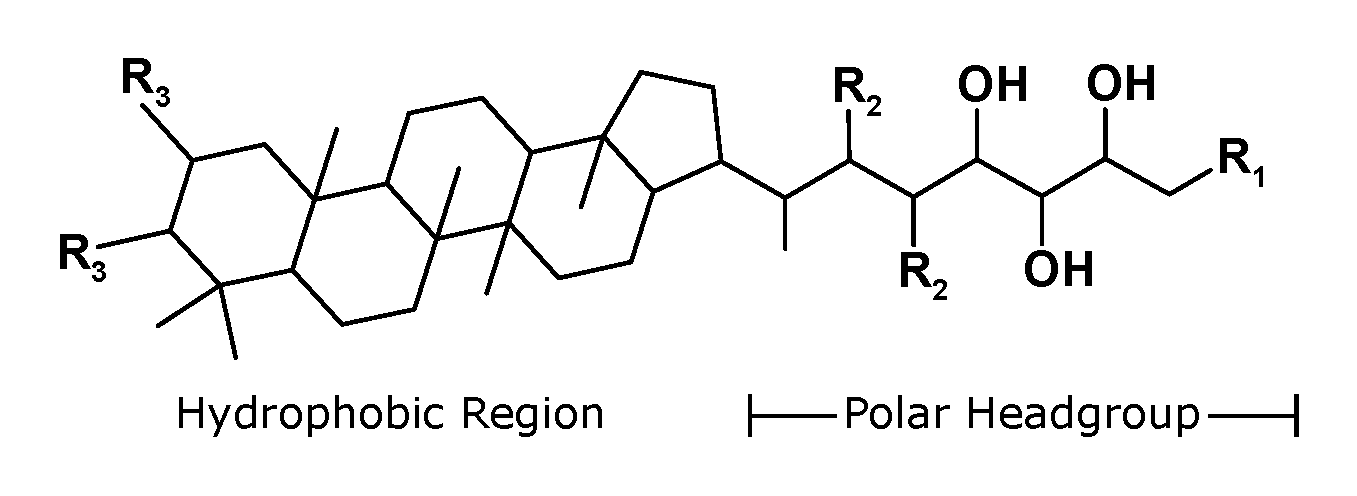
\includegraphics[width=1\linewidth]{figs_ch3/BHP_structure_general.pdf}
\caption[Generalized bacteriohopanepolyol chemical structure]{Generalized bacteriohopanepolyol (BHP) chemical structure. For BHPs without composite groups, R\textsubscript{1} represents a hydroxyl (OH), amine (NH\textsubscript{2}), or amminium (NH\textsubscript{3}\textsuperscript{+}) group. R\textsubscript{2} stands for H or OH. The BHP is considered pentafunctional if one R\textsubscript{2} is OH, or hexafunctional if both are OH. R\textsubscript{3} stands for H or CH\textsubscript{3}.}
\label{fig:BHP_structure}
\end{figure}
\doublespace




\singlespace
\begin{figure}[h]
\centering
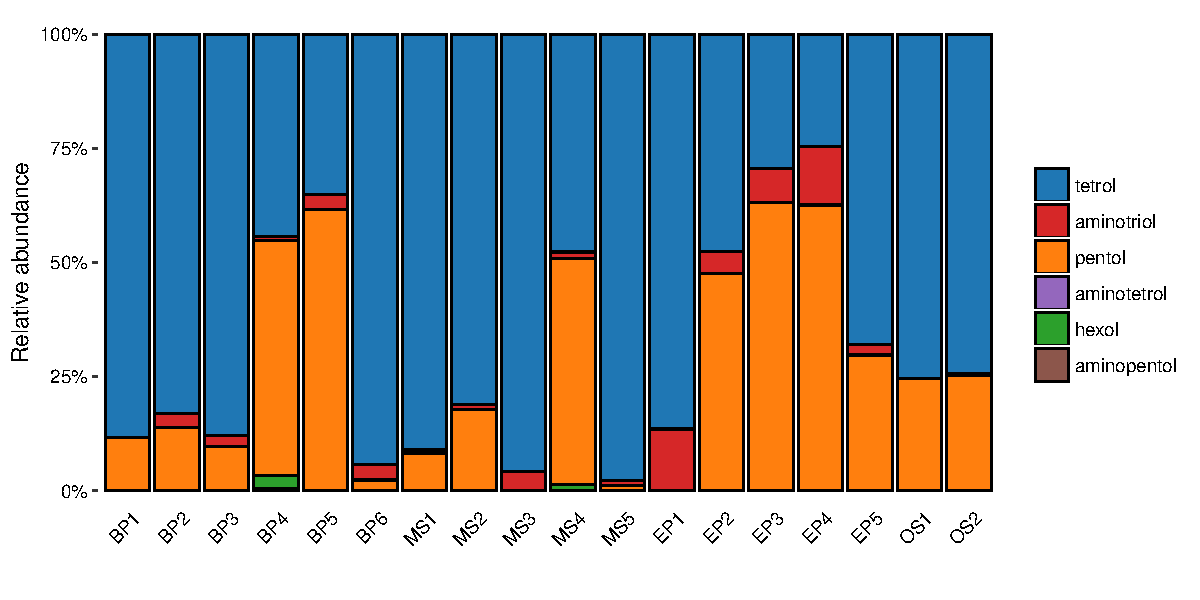
\includegraphics[width=1\linewidth]{figs_ch3/BHP_barchart.pdf}
\caption[Relative abundances of BHP polar headgroup functionality observed in Yellowstone hot spring sediments and biofilms]{Relative abundances of BHP polar headgroup functionality observed in Yellowstone hot spring sediments and biofilms.}
\label{fig:BHP_abund_Bison}
\end{figure}
\doublespace



\singlespace
\begin{figure}[h]
\centering
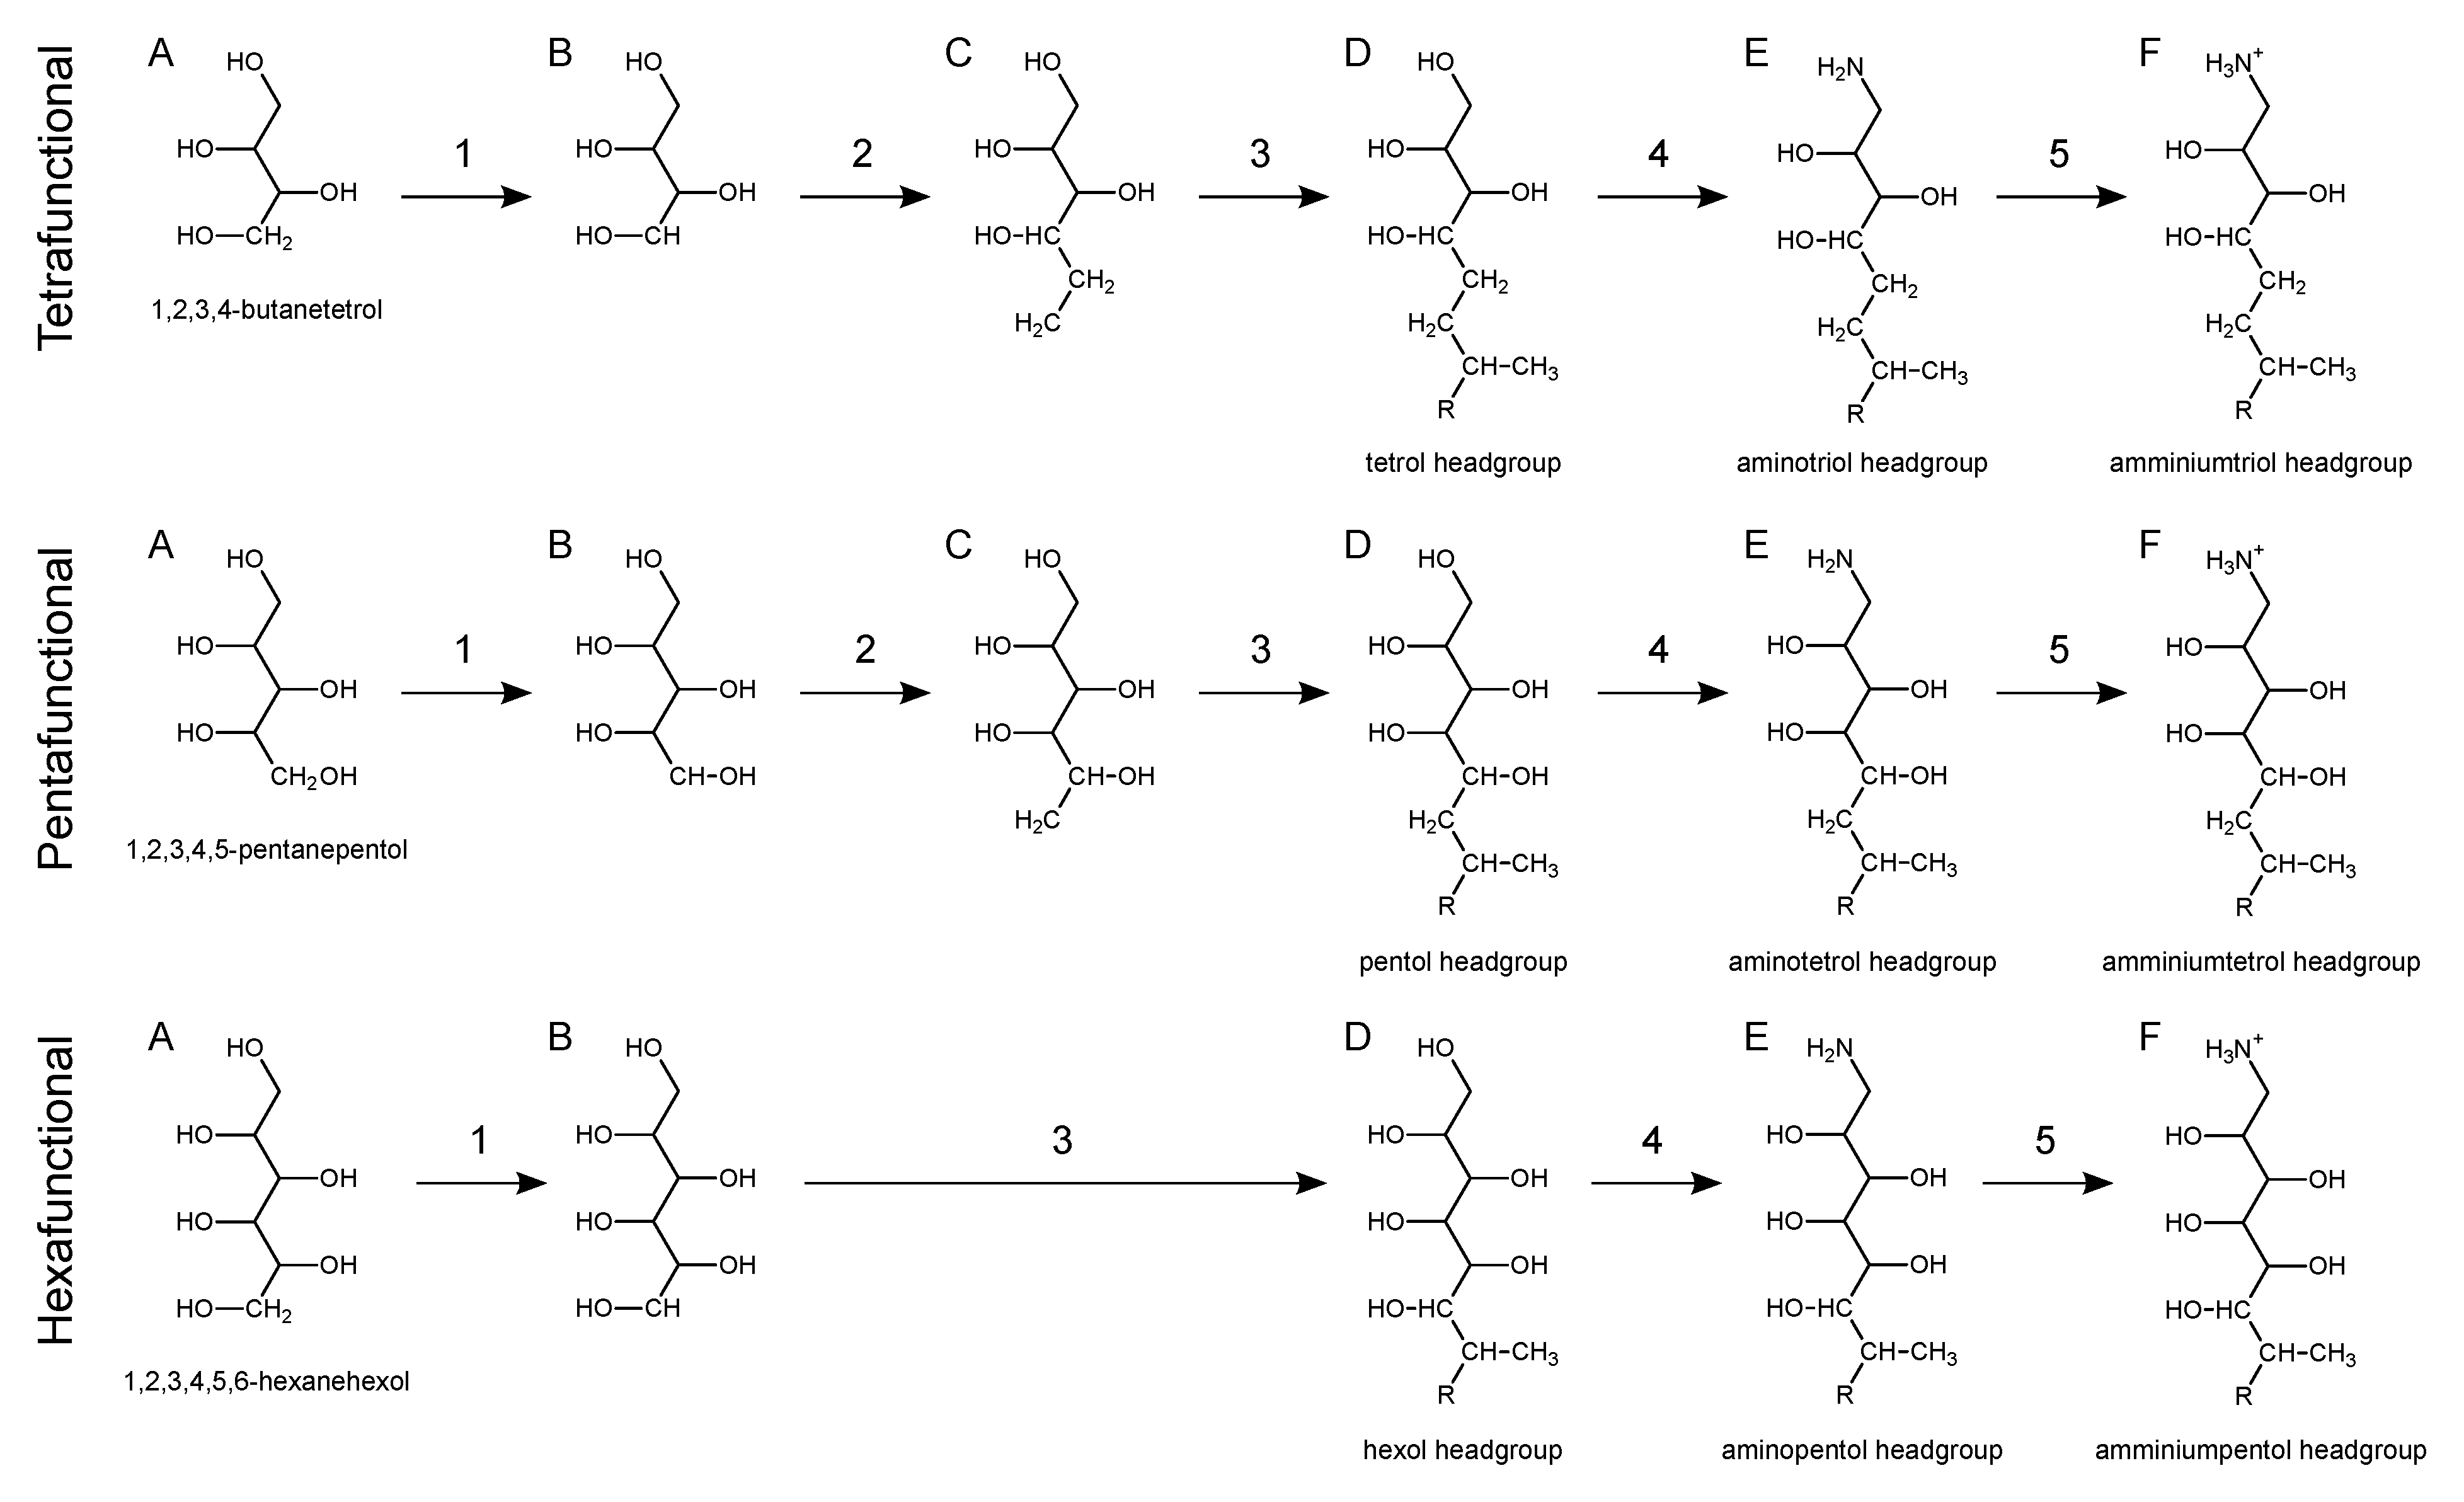
\includegraphics[width=1\linewidth]{figs_ch3/BHP_thermoest_paper.pdf}
\caption[Workflow used in the estimation of partial molal standard state thermodynamic properties of aqueous BHP headgroups]{Workflow used in the estimation of partial molal standard state thermodynamic properties of aqueous BHP headgroups. Structures and steps are described in the methods. R stands for the rest of the BHP structure, though its thermodynamic properties are not considered in this study.}
\label{fig:BHP_thermoest_paper}
\end{figure}
\doublespace


\singlespace
\begin{figure}[h]
\centering
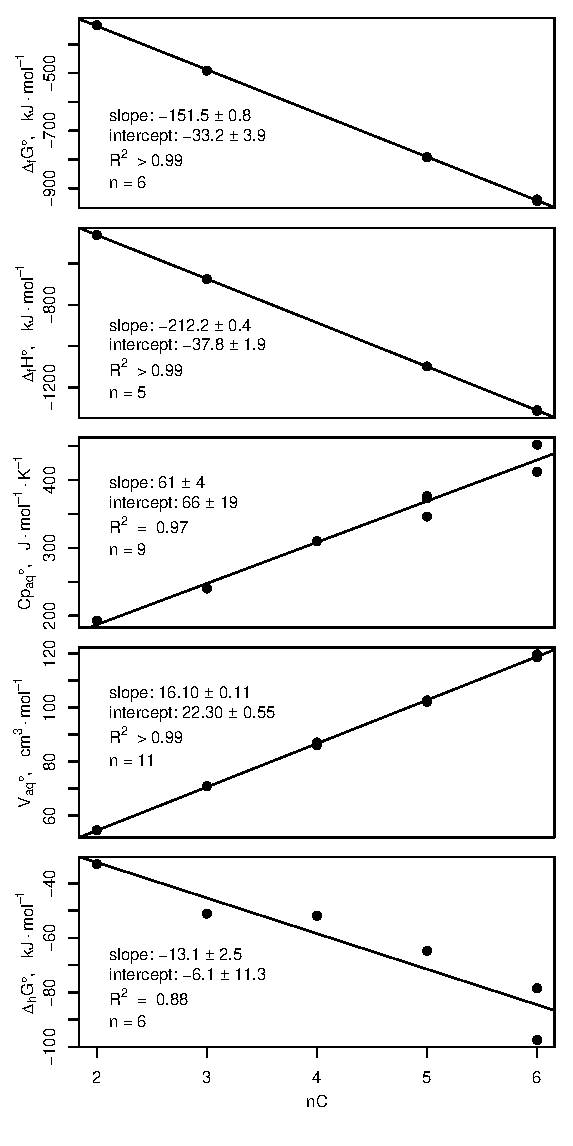
\includegraphics[width=0.5\linewidth]{figs_ch3/polyol_prop_regress.pdf}
\caption[Linear regression of experimentally-derived aqueous partial molal thermodynamic properties of sugar alcohols as a function of carbon length]{Linear regression of experimentally-derived aqueous partial molal thermodynamic properties of sugar alcohols as a function of carbon length (nC). Numbers of regressed datapoints for each plot are displayed equal to `n'. Literature sources for regressed data are given in Table \ref{tab:sug_alc}.}
\label{fig:polyol_prop_regress}
\end{figure}
\doublespace


\singlespace
\begin{figure}[h]
\centering
    \begin{subfigure}[b]{\linewidth}
        \includegraphics[width=\linewidth]{figs_ch3/"Bison OF1_BHP_mosaic"}
        \label{fig:BP1_degform}
    \end{subfigure}
    \begin{subfigure}[b]{\linewidth}
        \includegraphics[width=\linewidth]{figs_ch3/"Bison OF2_BHP_mosaic"}
        \label{fig:BP2_degform}
    \end{subfigure}
\end{figure}

\newpage

\begin{figure}[h]\ContinuedFloat
    \begin{subfigure}[b]{\linewidth}
        \includegraphics[width=\linewidth]{figs_ch3/"Bison OF3_BHP_mosaic"}
        \label{fig:BP3_degform}
    \end{subfigure}\\[-4ex]
    \begin{subfigure}[b]{\linewidth}
    	\includegraphics[width=\linewidth]{figs_ch3/"Bison OF4_BHP_mosaic"}
        \label{fig:BP4_degform}
    \end{subfigure}
\end{figure}

\newpage

\begin{figure}[h]\ContinuedFloat
    \begin{subfigure}[b]{\linewidth}
        \includegraphics[width=\linewidth]{figs_ch3/"Bison OF5_BHP_mosaic"}
        \label{fig:BP5_degform}
    \end{subfigure}
    \begin{subfigure}[b]{\linewidth}
        \includegraphics[width=\linewidth]{figs_ch3/"Bison OF6_BHP_mosaic"}
        \label{fig:BP6_degform}
    \end{subfigure}\\[-4ex]

\caption[lot cap]{cap}
\label{fig:degree_formation_bison}
\end{figure}
\doublespace




\singlespace
\begin{figure}[h]
\centering
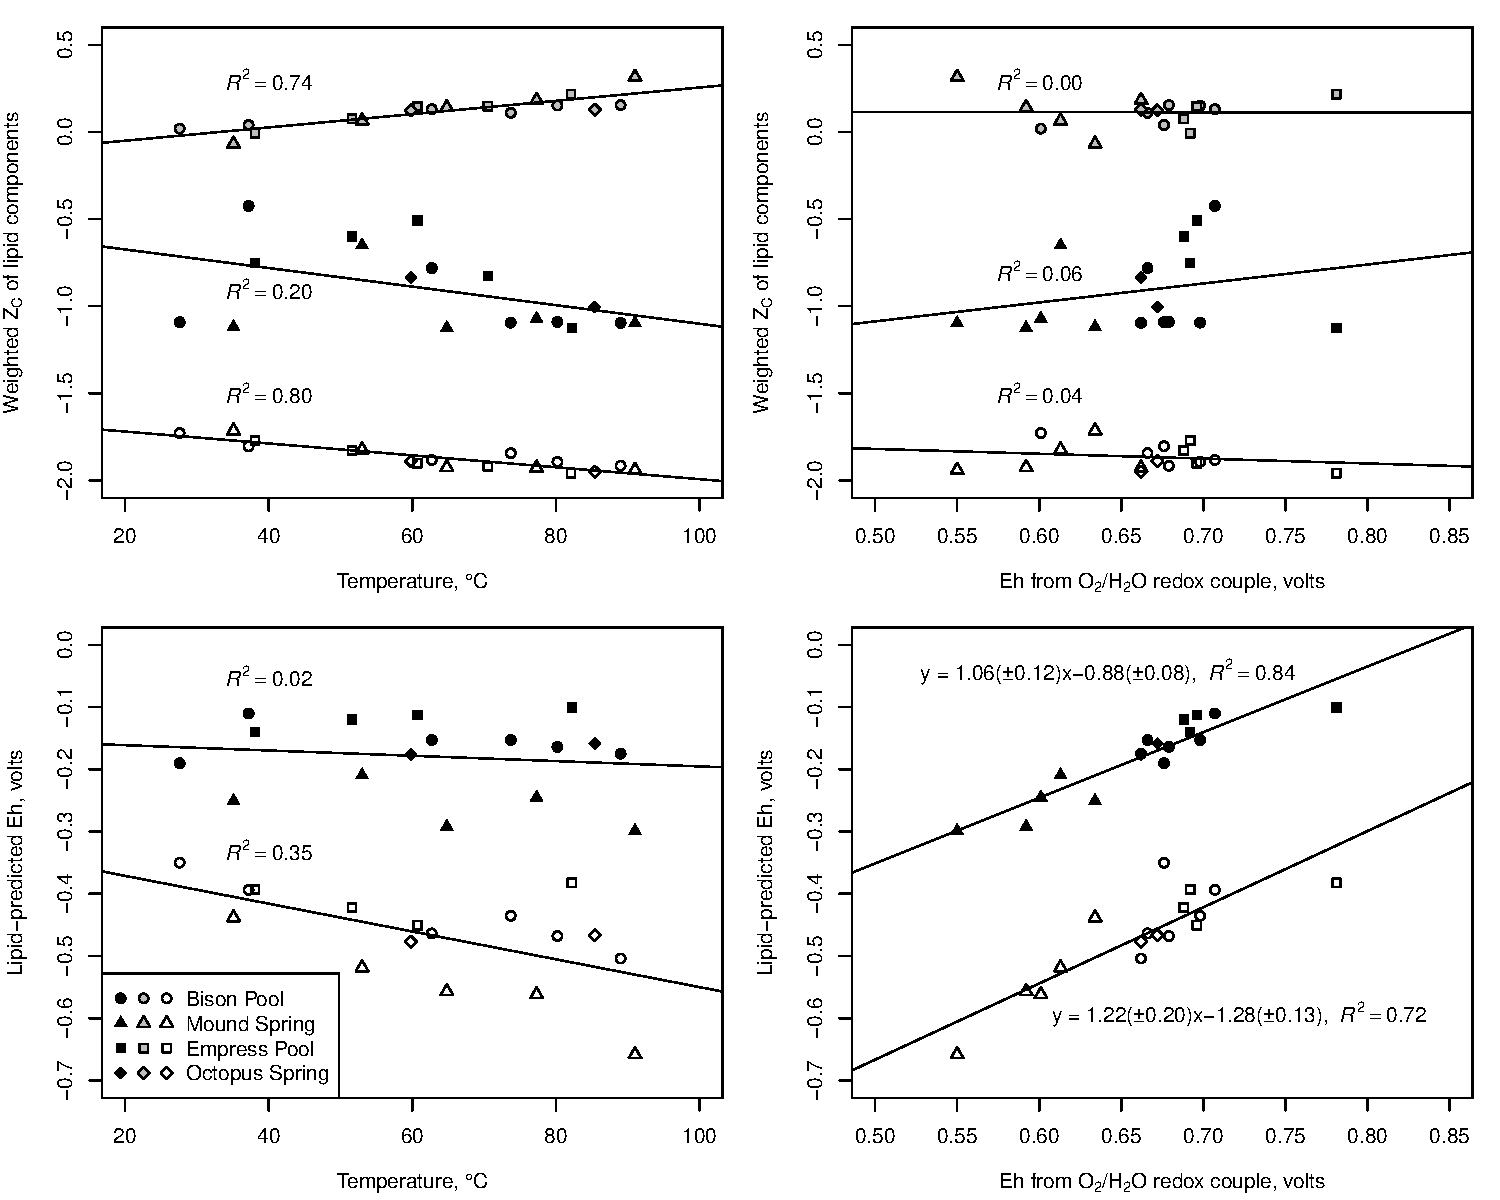
\includegraphics[width=1\linewidth]{figs_ch3/ZC_Eh_fourpanel.pdf}
\caption[Weighted Z\textsubscript{C} of thermophile lipid components and lipid-predicted Eh as a function of temperature and redox potential]{Weighted Z\textsubscript{C} of thermophile lipid components and lipid-predicted Eh as a function of temperature and redox potential. Black and gray symbols indicate headgroups of BHPs and IPLs, respectively. White/empty symbols indicate IPL alkyl chains in the upper plots or site-averaged IPL alkyl chains in the lower plots. Values for Z\textsubscript{C} of IPL components and alkyl chain-predicted Eh are taken from Chapters \ref{ch1} and \ref{ch2}, respectively. Standard errors of slopes and intercepts of linear fits are shown in parentheses and do not include propagated uncertainties from underlying thermodynamic estimations. Unweighted linear models were used to generate R\textsuperscript{2} values.}
\label{fig:ZC_Eh_fourpanel}
\end{figure}
\doublespace
\chapter[CONCLUSION]{Conclusion}

\section{Summary}

Organisms require functioning lipids across the entire range of conditions where life is found. As a result, there is an enormous variety of lipid adaptations in biology. As was discussed in this dissertation, however, certain lipid structures are known to function effectively in very different sets of environmental conditions; \textit{e.g.}, glycerol dialkyl glycerol tetraethers (GDGTs) can create stable lipid membranes in both thermophiles and mesophiles \citep{schouten2000widespread}. Likewise, very different sets of lipid distributions may function effectively in the similar environmental conditions; \textit{e.g.}, GDGTs or non-GDGTs can create stable lipid membranes in mesophiles. Any given lipid adaptation, whether it is a double bond, a longer alkyl chain, or a particular headgroup, will have an energetic cost associated with its biosynthesis. These costs are predicted to change depending on the temperature, pressure, and chemical context of the surroundings.

This work provided evidence to support the hypothesis that natural selection favors convergence upon lipid compositions that maximize function while also minimizing energetic cost. First, the abundance-weighted Z\textsubscript{C} of lipids sampled from microorganisms from four alkaline hot springs was shown to correlate positively with the oxidation state of the environment. Adaptations to provide alkyl chain functionality and membrane fluidity were themselves oxidized under oxidized conditions and reduced under reduced conditions, which I hypothesized was energetically cost-efficient. A subsequent thermodynamic analysis provided evidence to support this hypothesis for intact polar lipid (IPL) alkyl chains by predicting that observed IPL distributions were stable relative to each other along redox gradients. Additionally, values of Eh predicted to result in favorable alkyl chain distributions were predicted to be correlated positively with environmental Eh. Lipid headgroups were also investigated and yielded results similar to those of alkyl chains; that hot spring Eh was correlated positively with Eh predicted by energetically stable configurations of observed headgroup ratios. In sum, this work suggests structural adaptations in lipid distributions are not only present because they function for their source organisms, but because they are cost-effective to produce within the temperature and geochemical context of their surroundings.

The thermodynamic studies described in this dissertation did not include calculations involving individual reactions of biosynthesis pathways or intracellular concentrations of chemical species in their evaluation of lipid cost. Instead, net reactions to form lipids from measured concentrations of bioavailable solutes alone provided evidence that observed thermophile lipid distributions may be energetically cost-effective. It is essential for cells to regulate intracellular conditions such as pH and solute concentrations for metabolic pathways to proceed. Maintaining chemical disequilibrium from the external environment requires energy. However, I would argue this energy requirement is based on how well a cell is adapted to its surroundings; energetic shortcuts to synthesize necessary biomolecules from available materials in the surroundings would offset a portion of this energy requirement. This raises the possibility that conditions \textit{outside} of the cell matter more for the energetic costs of biomolecules than the conditions \textit{inside} the cell. This concept could serve as a foundation for studies in molecular biology to evaluate potential costs of biomolecules synthesized by microbial communities in a variety of natural systems and in culture.

\section{Future Work}

Studies of lipid distributions in natural systems could be mainly exploratory (\textit{i.e.}, which lipids are found under which sets of geochemical conditions) but could be supplemented by calculation of Z\textsubscript{C} or thermodynamic predictions to allow quantitative assessment of lipid distributions in terms of energetic cost. These studies could also consider the phylogeny of source organisms, which was not done here. For instance, would a cyanobacteria-dominated microbial community that is adapted to thrive in water rich in hydrogen and methane, such as conditions found in fluids discharged from serpentinizing systems \citep{mccollom2009thermodynamic}, tend to produce lipid compositions with reduced carbon relative to cyanobacteria-dominated communities in oxidized ocean surface water? How phylogenetically related can two microbial communities be while having drastically different lipid compositions, and how might functional necessity and energetic cost help explain these differences?

These types of questions could also be probed in laboratory experiments. Various growth media of known chemical compositions could be inoculated with a mixed culture to isolate sub-sets of microbes that grow best under those conditions. Thermodynamic calculations based on those described in this work might then be used to predict whether the lipid compositions of isolated sub-sets tend to be energetically favorable in the chemical conditions of their own growth media relative to all others in the experiment. Would thermodynamic predictions offer greater insight into the expression of observed lipid distributions in these various treatments than the phylogenetic compositions of the isolated microbial sub-sets?

Future studies should attempt to be as quantitative as possible when measuring lipid abundances to allow estimation of weighted molecular properties like the average oxidation state of carbon (Z\textsubscript{C}) or partial molal thermodynamic properties such as Gibbs free energies of formation, volumes, entropies, and the like. The power to describe lipid distributions with of Z\textsubscript{C} or thermodynamic calculations depends on the physical and chemical parameters of the system. As such, I recommend that these studies strive to be as complete as possible when measuring temperature, pressure, and chemical composition of the natural system or growth media.

Thermodynamic calculations could explore the formation of lipids from a different set of basis species than the `autotrophic' set used in this work. It may be more appropriate to use acetate, for instance, to predict lipid distributions in a predominantly heterotrophic microbial community. Future studies could focus on reducing sources of error to aid in the comparison of thermodynamically predicted and analytically observed lipid abundances. Constraining sources of error introduced by lack of authentic response factors may offer a better estimation of aminopolyol BHP abundance. Alternate estimation schemes could be explored to estimate lipid thermodynamic properties. Liquid-phase or crystalline-phase alkyl chains, or a combination of the two, could be included in formation reactions from aqueous basis species to simulate the formation of a membrane lipid; this may offer a better predictive model than the formation of free aqueous lipids. Alternative methods for predicting complex distributions of lipids from basis species could be explored, and results could be compared to outcomes produced by the hypothetical site-averaged chains.

% extras, if needed:
% Lipid studies addressing "maximization of function". Assumed, but not tested here. Some studies have addressed function (e.g. SQ headgroups and ability to photosynthesize, or knockout membranes with no BHPs, etc.)

\section{Broader Impacts}

Interpreting the expression of lipids in terms of functional benefit and energy cost has the potential to change our understanding of the evolution of lipids, geochemical controls on lipid distributions, and ultimately how biomarkers are interpreted in the rock record.

Biochemistry emerged from geochemical processes, though it is still unclear when lipids emerged in the history of life. Some theories posit that lipids were essential for metabolic encapsulation, growth, and division in the first proto-organisms \citep{deamer2002first, luisi2016emergence}. Placing abiotic lipid synthesis in a thermodynamic framework could help narrow down geochemical conditions conducive to spontaneous lipid formation that could then be reconciled with the conditions proposed to allow early growth and division. It has also been theorized that lipid membranes evolved later.  These theories hold that the last universal common ancestor (LUCA) that led to modern Bacteria, Archaea, and Eukarya lacked lipid membranes \citep{koga1998did, martin2003origins}, or had membranes with simpler lipid compositions \citep{sojo2014bioenergetic}. The notion that biology maximizes lipid function and minimizes energy cost could be applied to aid understanding of evolutionary pressures imposed by geochemistry that led to the divergence of lipid synthesis pathways among prokaryotes and eukaryotes after LUCA. While these are meant to represent specific examples where lipids are the focus, I am optimistic that thermodynamic assessments of the energetic costs of biomolecules would benefit evolutionary studies in general.

% geochemical controls on lipid distributions. Frame in astrobiological sense. Function of new lipid structures still under invest, but thermo predictions could help uncover sources.

Lipid biomarkers have great potential to reveal detail about the environmental conditions experienced by their source communities, as well as geochemistry experienced by sedimentary rocks after diagenesis. In \cite{ourisson1979hopanoids}, the authors report complex distributions of hopanoid lipid degradation products from a variety of sediments. They reported that hundreds of chemical structures were observed in these biomarkers, ranging from carboxylic acids to aldehydes to hydrocarbons to aromatic compounds, and emphasized that a wealth of information about geologic history could be unlocked if more could be learned about geochemical influences on the transformation of biomarkers. A review by \cite{ourisson1992hopanoids} included speculation about patterns in hopanoid degradation products expected to form under oxidized and reduced conditions, but without a thermodynamic framework, these patterns can only be interpreted qualitatively. This dissertation focused on thermal and geochemical controls on lipid expression in active, living systems, but thermodynamic data could be expanded to include biomarker degradation products. Thermodynamic calculations could potentially revolutionize the interpretation of biomarkers by allowing quantitative predictions regarding the chain of geologic events that led to observed biomarker distributions in the rock record.

\section{Concluding Remarks}
Geochemistry dictates what is necessary for habitability. This dissertation explored what that means for lipid adaptation; a lipid composition must function within the conditions experienced by the microbial community that produced it, and it must also have an acceptable energetic cost. This energetic cost is dictated by the temperature, pressure, and chemical composition of the system. A microbial community adapted to its surroundings is one that has evolved lipid distributions that are both functional and cost-effective. The composition of lipid structures produced by a microbial community should therefore reflect this interplay of energetic cost and functional benefit. Energetic cost can be assessed quantitatively, but this requires a thermodynamic framework to work within. This dissertation provides a step in that direction. Future work aimed at developing this framework further has the potential to shed great insight into why life produces the chemical structures that it does; not only with respect to lipid adaptation in thermophiles but for biomolecular adaptation across all of biology.

% how lipid composition in eukaryotic organelles may have evolved over time.

% paleothermometry - paleoredox

%Everett wrote for NSF proposal: The development of thermodynamic data for lipid biomolecules and their biomarker degradation products will unlock the record of geochemical transformations recorded in these compounds, which will test, confirm, and challenge conclusions drawn from mineralogical, isotopic, and trace element datasets from sedimentary rocks. It is possible that biomarkers will become as useful for deciphering the geological history of sedimentary rocks as they are presently for determining the depositional environments of the original sediments.
%Biomarkers hold the potential to reveal extraordinary detail about past environmental conditions that prevailed anywhere that sediments accumulate and preserve geobiochemical information. There is an impressive potential for a comprehensive understanding of global change through integrating biomarkers with many other lines of evidence from the geological record. Remarkably, biomarker research is predominantly an analytical pursuit with few experimental studies and even fewer efforts at a theoretical framework. This project will provide a foundation for that framework, which will yield novel applications in microbial physiology, evolution of biochemical pathways, climate change, and the emerging field of geobiochemistry


% Concluding remarks suggested by committee:
% Potential applications: interpretation of lipid distributions in the rock record and their controls and eventually interpreting how lipid distributions are altered after deposition; Predicting which lipid biomarkers to target in astrobiology missions; New insight into the evolution of lipids in biology. Future work could compare lipid thermo calcs to (meta)genomes to show that bioenergetic trends exist regardless of organisms.

% astrobiology impact: cite paper about lipid patterns in astrobio I sent to Melissa.





%-----------------------back matter
{\singlespace
% Making the references a "part" rather than a chapter gets it indented at
% level -1 according to the chart: top of page 4 of the document at
% ftp://tug.ctan.org/pub/tex-archive/macros/latex/contrib/tocloft/tocloft.pdf
\addcontentsline{toc}{part}{REFERENCES}
\bibliographystyle{asudis}
\bibliography{dis}}
\renewcommand{\chaptername}{APPENDIX}
\addtocontents{toc}{APPENDIX \par}
\appendix
\chapter{Intact polar lipid response factors and mass spectral interpretation of novel structures}\label{app1}

\clearpage

\doublespace

\paragraph*{Analytical response factors.} Table \ref{tab:RF} gives information about response factors for the suite of intact polar lipid (IPL) standards used in this work. Response factors were interpreted as the linear slopes of high-performance liquid chromatography-mass spectrometry (HPLC-MS) integrated peak area as a function of injected mass with a y-intercept of zero. The squared correlation coefficient, $R^{2}$, is reported for each regression. Two sets of response factors are given, one for a sample batch run in 2013 and another in 2014. Samples MS1, MS3, MS4, and MS5 use the response factors for 2014, while all other samples use those for 2013.

\paragraph*{Mass spectral interpretation of novel structures.} Mass spectra and putative chemical structures of lipids identified in this work are shown in Figures \ref{fig:MeNG-G-P-AR} through \ref{fig:G-GA-DAG}. All lipid structures shown here are tentatively assigned based on MS/MS fragmentation patterns. Carbon positions of alkyl chain modifications, bonding, and configuration between glycolipid headgroup moieties, \textit{etc.}, are guesses. Dotted arrows refer to inferred fragmentation of the displayed structure and point in the direction of the fragment with the monoisotopic mass, in Da, listed at the end of the arrow. pNLC stands for `precursor neutral loss chromatogram'. This is a method for searching for an MS/MS chromatogram based on the difference between the mass of a lipid precursor ion before and after the loss of a diagnostic fragment; usually in the case of IPLs, this is the headgroup or a piece of the headgroup. M+H and M-H refer to the monoisotopic mass of the displayed structure plus or minus a hydrogen atom, respectively, and assumes that the resulting fragment has an overall charge of +1.

\clearpage

\afterpage{
\singlespace
\begin{table}
\centering
\begin{threeparttable}
  \caption{HPLC-MS IPL standards and response factors}
 
% Table generated by Excel2LaTeX from sheet 'RF info (2)'
\begin{tabular}{rllrrrr}
\toprule
      &       &       & \multicolumn{2}{c}{Batch 1\tnote{b}} & \multicolumn{2}{c}{Batch 2\tnote{c}} \\
\cmidrule(l{2pt}r{2pt}){4-5} \cmidrule(l{2pt}r{2pt}){6-7}No.\tnote{a} & Standard & Chains & RF    & \textit{R\textsuperscript{2}} & RF    & \textit{R\textsuperscript{2}} \\
\midrule
1     & 1Gly-DAG & mix of C34:6, C36:6 & 6.37$\times 10$\textsuperscript{5} & 0.95  & 9.45$\times 10$\textsuperscript{5} & 0.99 \\
2     & 1Gly-GDGT-PG & mix of 0-3 rings, & 6.72$\times 10$\textsuperscript{4} & 0.96  & 1.16$\times 10$\textsuperscript{4} & 0.91 \\
      &       & $\sim$20\% H-shaped &       &       &       &  \\
3     & PC-DAG & C42:0 & 7.31$\times 10$\textsuperscript{5} & 0.99  & 2.71$\times 10$\textsuperscript{5} & 0.91 \\
4     & 2Gly-DAG & mix of C34:2, C34:3 & 1.33$\times 10$\textsuperscript{5} & 0.99  & 9.90$\times 10$\textsuperscript{4} & 0.99 \\
      &       & C34:6, C36:6 &       &       &       &  \\
5     & SQ-DAG & mix of C34:2,  & 1.31$\times 10$\textsuperscript{5} & 0.95  & 1.90$\times 10$\textsuperscript{5} & 0.99 \\
      &       & C34:3, C36:6 &       &       &       &  \\
6     & PI-DAG & C32:0 & 7.94$\times 10$\textsuperscript{3} & 0.88  & 5.95$\times 10$\textsuperscript{3} & 0.99 \\
7     & DPG   & C72:4 & 3.97$\times 10$\textsuperscript{5} & 0.95  & 7.24$\times 10$\textsuperscript{4} & 0.99 \\
8     & PDME-DAG & C32:0 & 1.11$\times 10$\textsuperscript{6} & 0.97  & 1.96$\times 10$\textsuperscript{6} & 0.99 \\
9     & PE-DAG & C32:0 & 4.06$\times 10$\textsuperscript{5} & 0.99  & 2.92$\times 10$\textsuperscript{5} & 0.95 \\
10    & PG-DAG & C32:0 & 1.49$\times 10$\textsuperscript{5} & 0.98  & 1.02$\times 10$\textsuperscript{5} & 0.99 \\
11    & PME-DAG & C32:0 & 5.45$\times 10$\textsuperscript{5} & 0.94  & 5.93$\times 10$\textsuperscript{5} & 0.99 \\
12    & PS    & C32:0 & 2.03$\times 10$\textsuperscript{4} & 0.98  & 2.30$\times 10$\textsuperscript{4} & 0.97 \\
13    & DGTS-d9 & C32:0 & 1.65$\times 10$\textsuperscript{6} & 0.89  & 7.16$\times 10$\textsuperscript{6} & 0.96 \\
\bottomrule
\end{tabular}%



\begin{tablenotes}
\small
\item [a] Corresponds to numbered standards in Table \ref{tab:IPL} of main text.
\item [b] Batch 1 was analyzed in 2013 and includes all Bison Pool, Empress Pool, and Octopus Spring samples, as well as Mound Spring sample MS2. Linear response factors and \textit{R\textsuperscript{2}} taken from two replicate calibrations of 0.1, 0.5, 1, 5, 10, and 50 ng standard injections.
\item [c] Batch 2 was analyzed in 2014 and includes Mound Spring samples MS1, MS3, MS4, and MS5. Linear response factors and \textit{R\textsuperscript{2}} taken from a single calibration of 0.1, 0.5, 1, 5, and 10 ng standard injections.

\end{tablenotes}

  \label{tab:RF}
  \end{threeparttable}
\end{table}

% replace \cmidrule{4-7} with:
% \cmidrule(l{2pt}r{2pt}){4-5} \cmidrule(l{2pt}r{2pt}){6-7}
\doublespace
\clearpage
}


\afterpage{
\singlespace
\begin{figure}[h]
\centering
    \begin{subfigure}[b]{1\linewidth}
       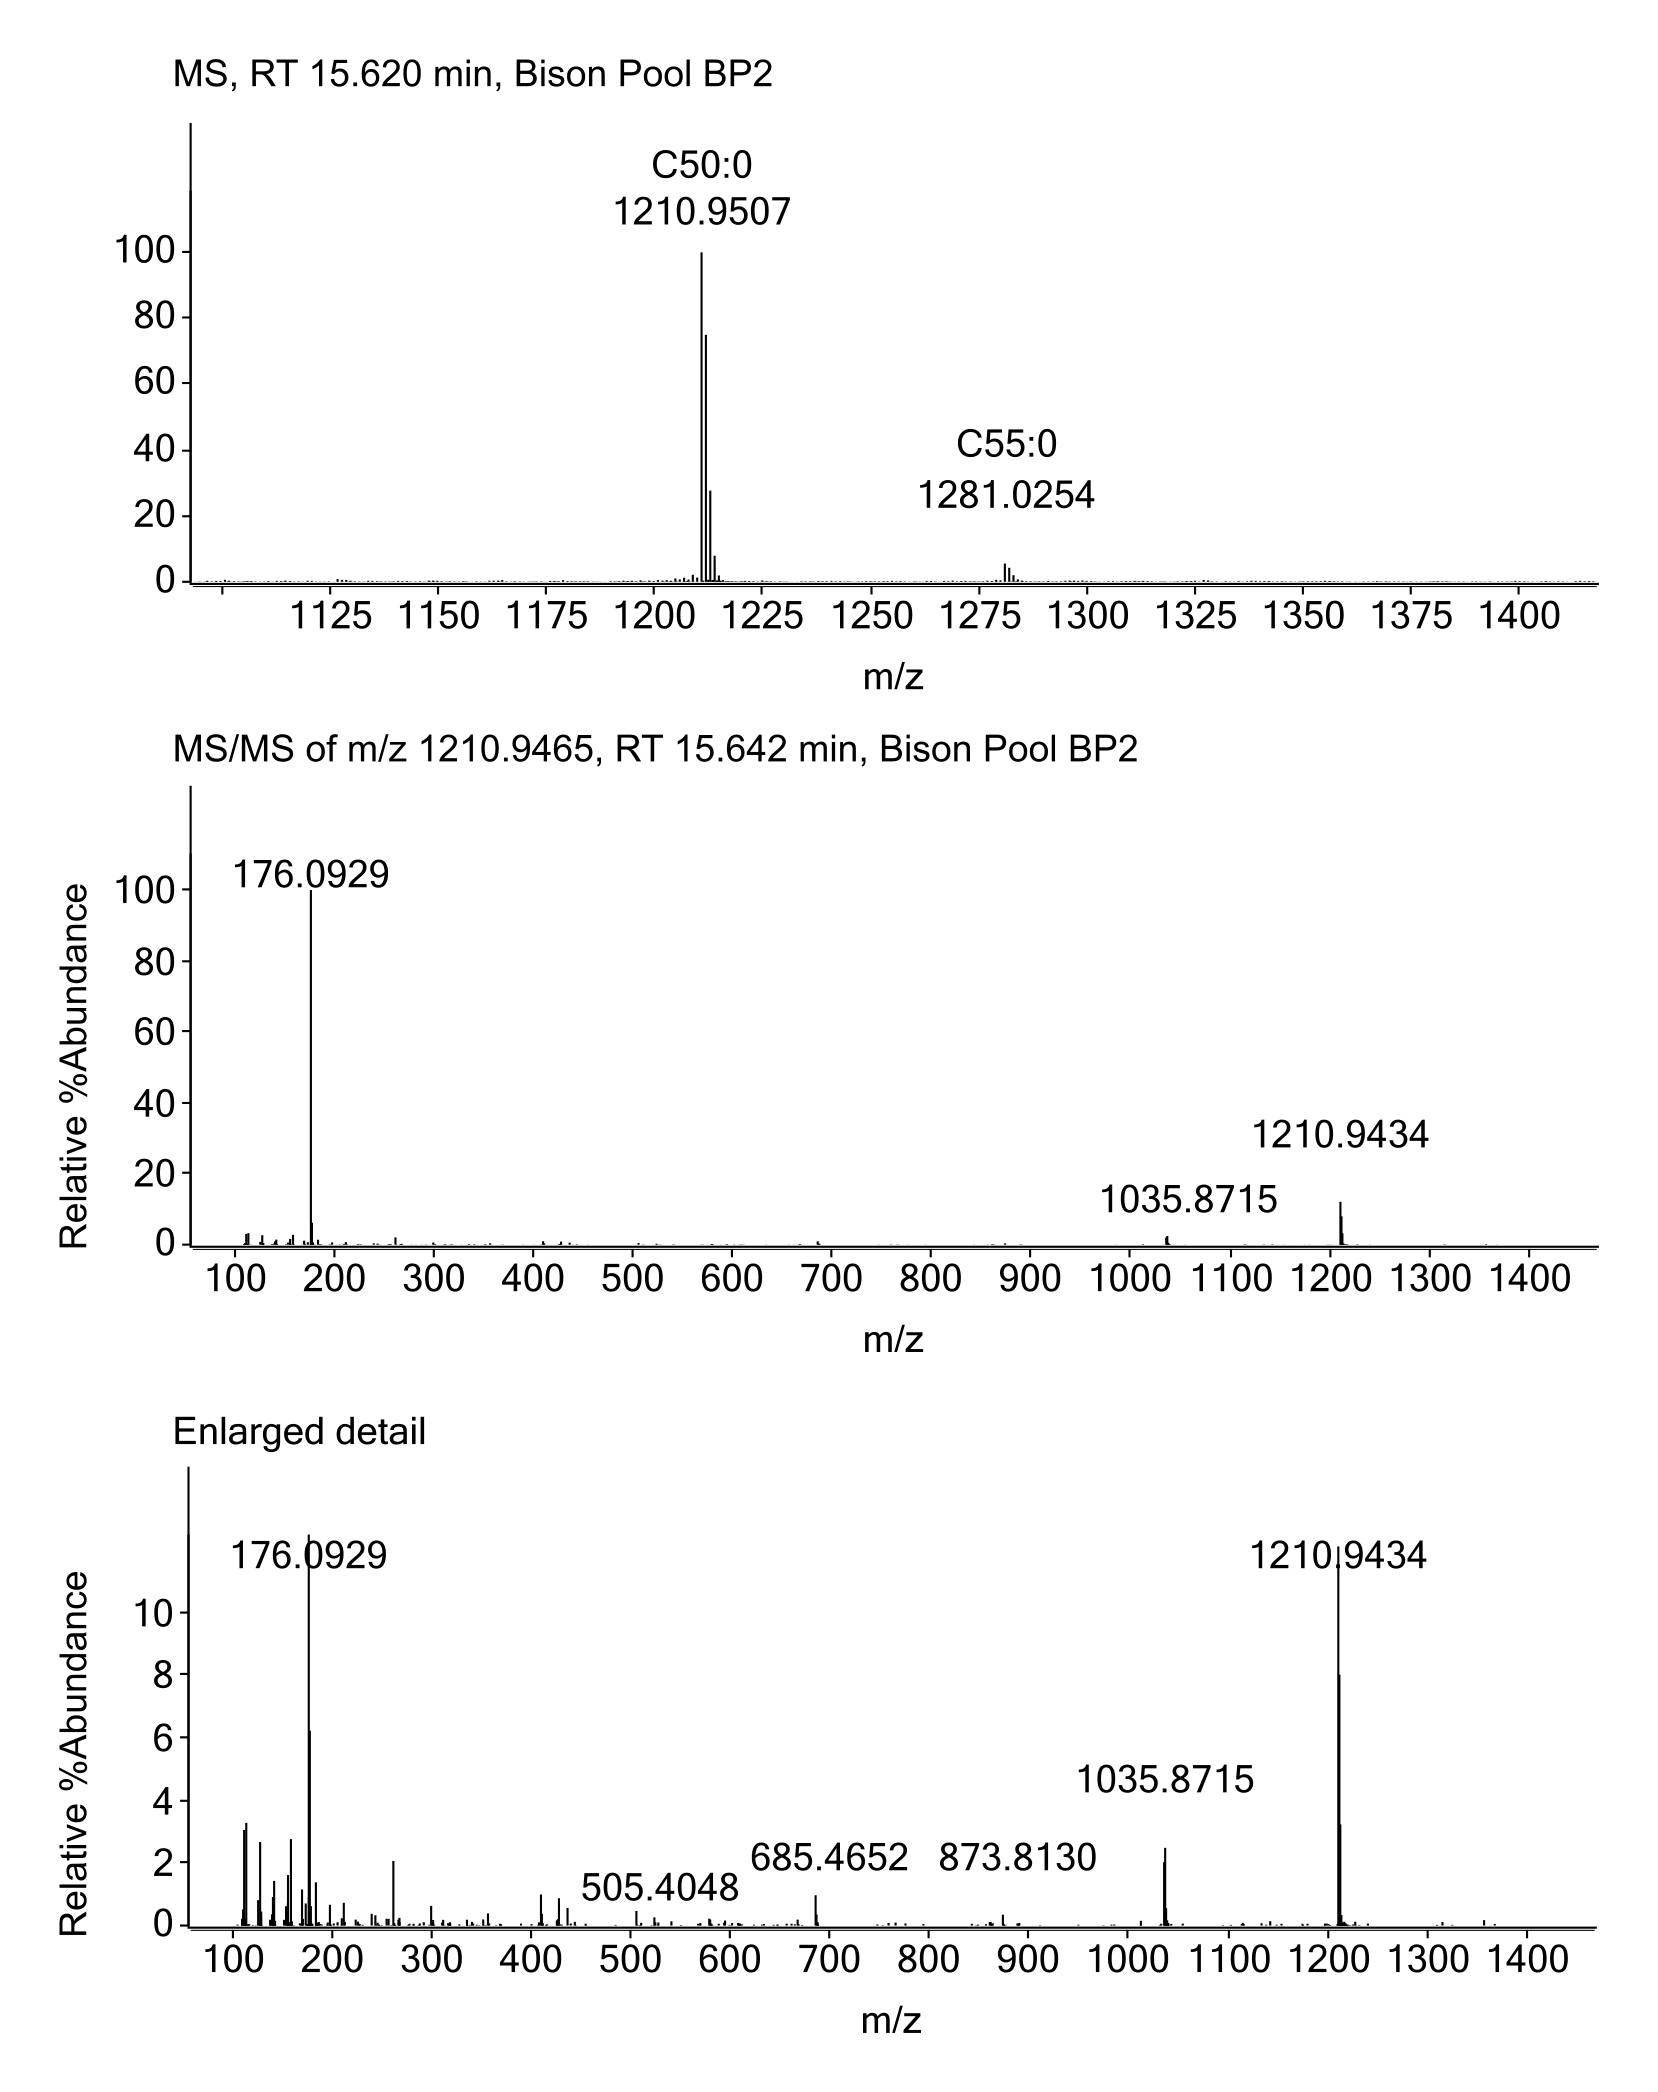
\includegraphics[width=\linewidth]{figs_app1/MeNG-G-P-AR_1}
       \caption{mass spectra}
        \label{fig:gull}
    \end{subfigure}
\end{figure}
\newpage
\begin{figure}[h] \ContinuedFloat
    \begin{subfigure}[b]{1\linewidth}
       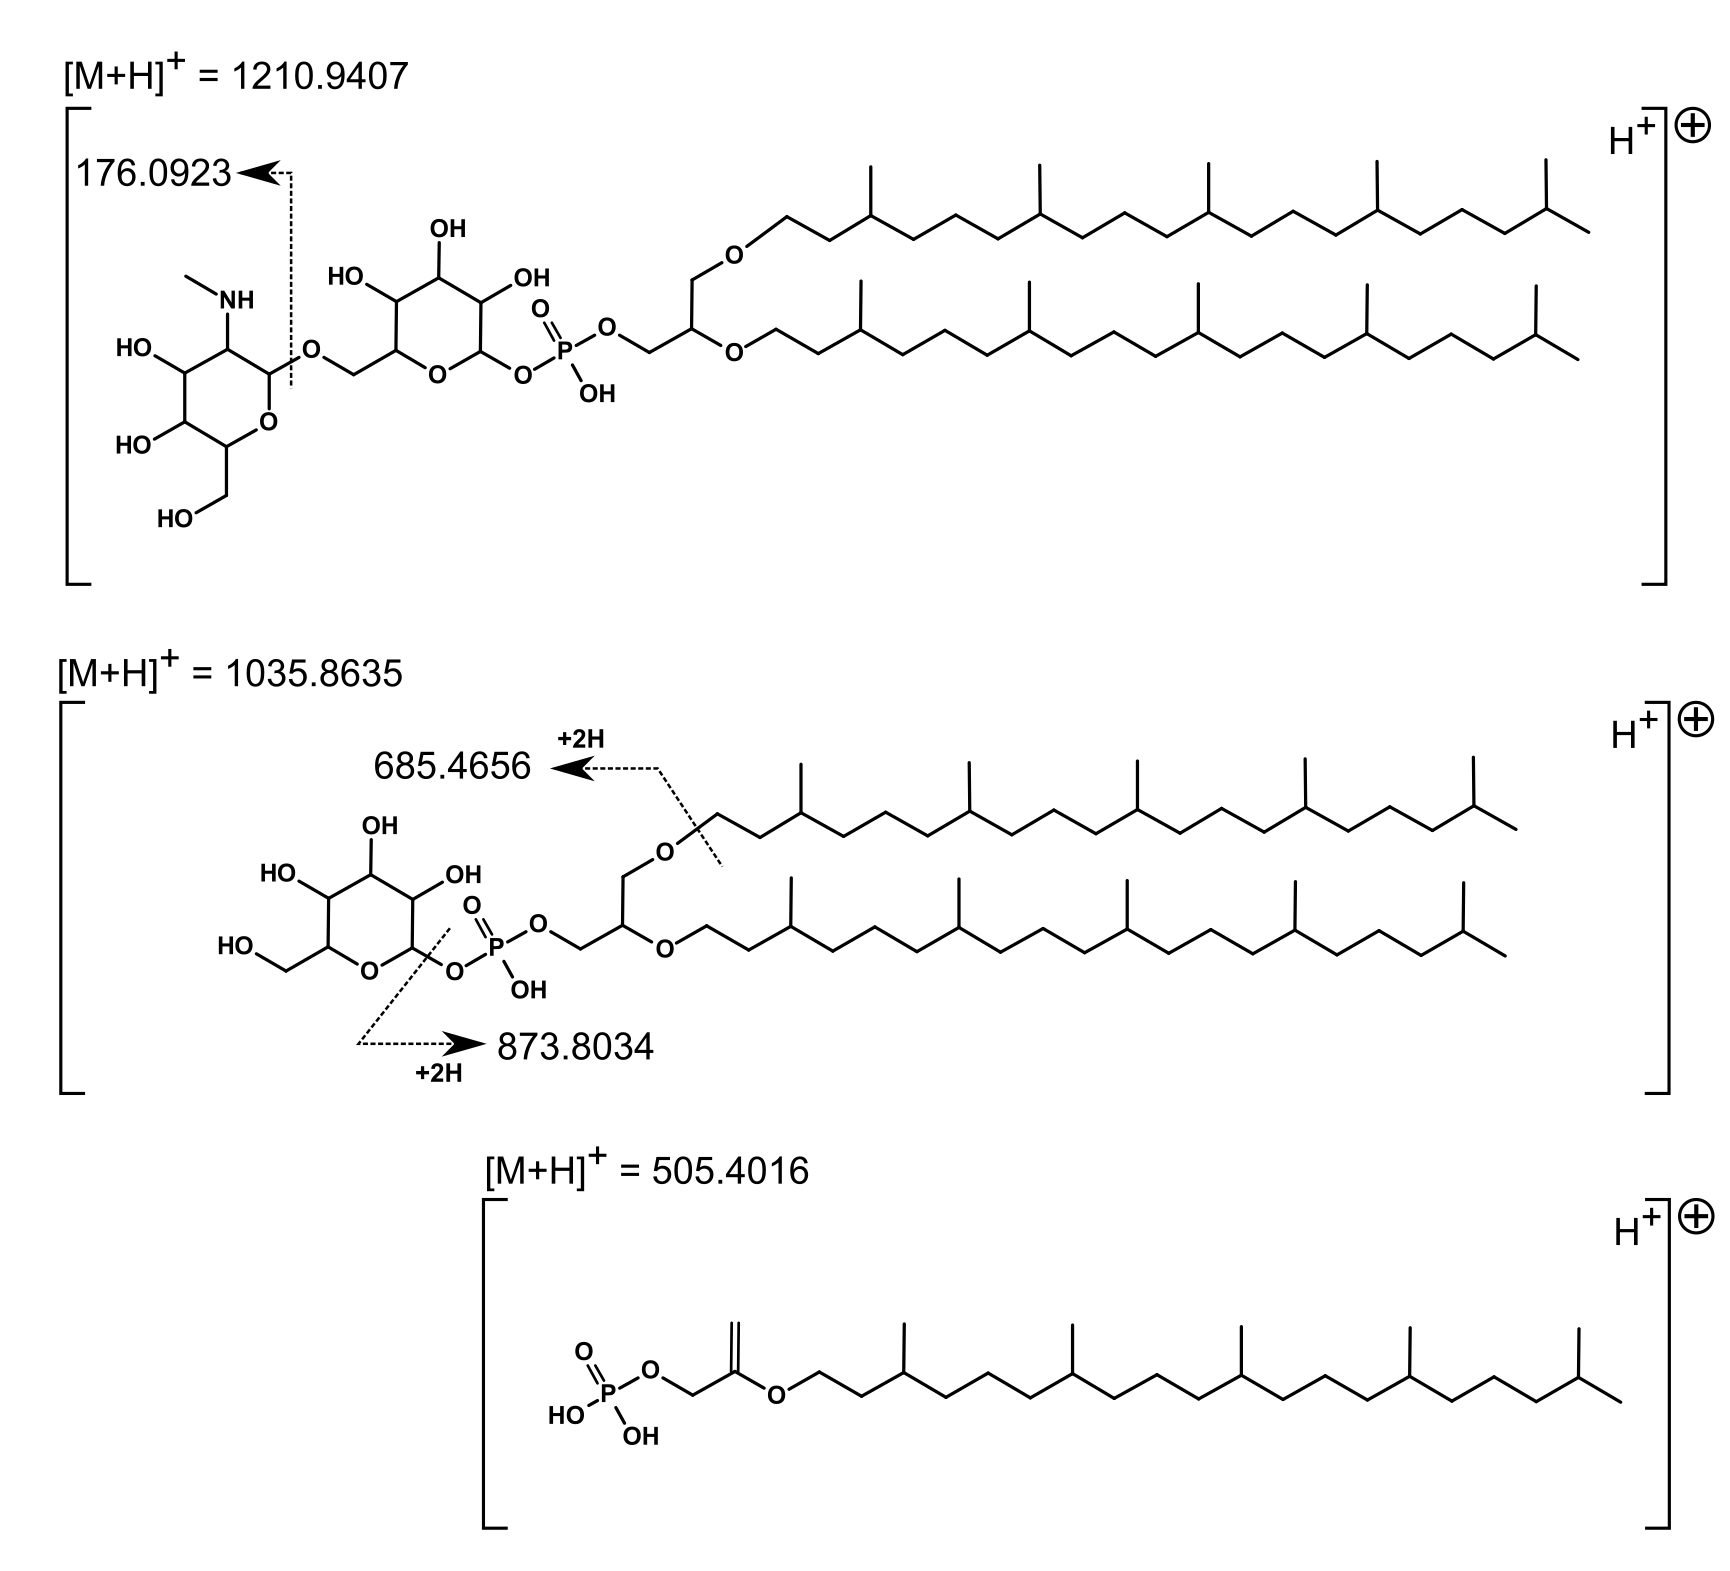
\includegraphics[width=\linewidth]{figs_app1/MeNG-G-P-AR_2}
       \caption{putative fragments}
        \label{fig:gull}
    \end{subfigure}
\caption{Mass spectra and putative structure for (N-methyl)glycosaminyl monoglycosyl phosphatidylarchaeol (MeNG-G-P-AR).}
\label{fig:MeNG-G-P-AR}
\end{figure}
\doublespace
\clearpage
}

\afterpage{
\singlespace
\begin{figure}[h]
\centering
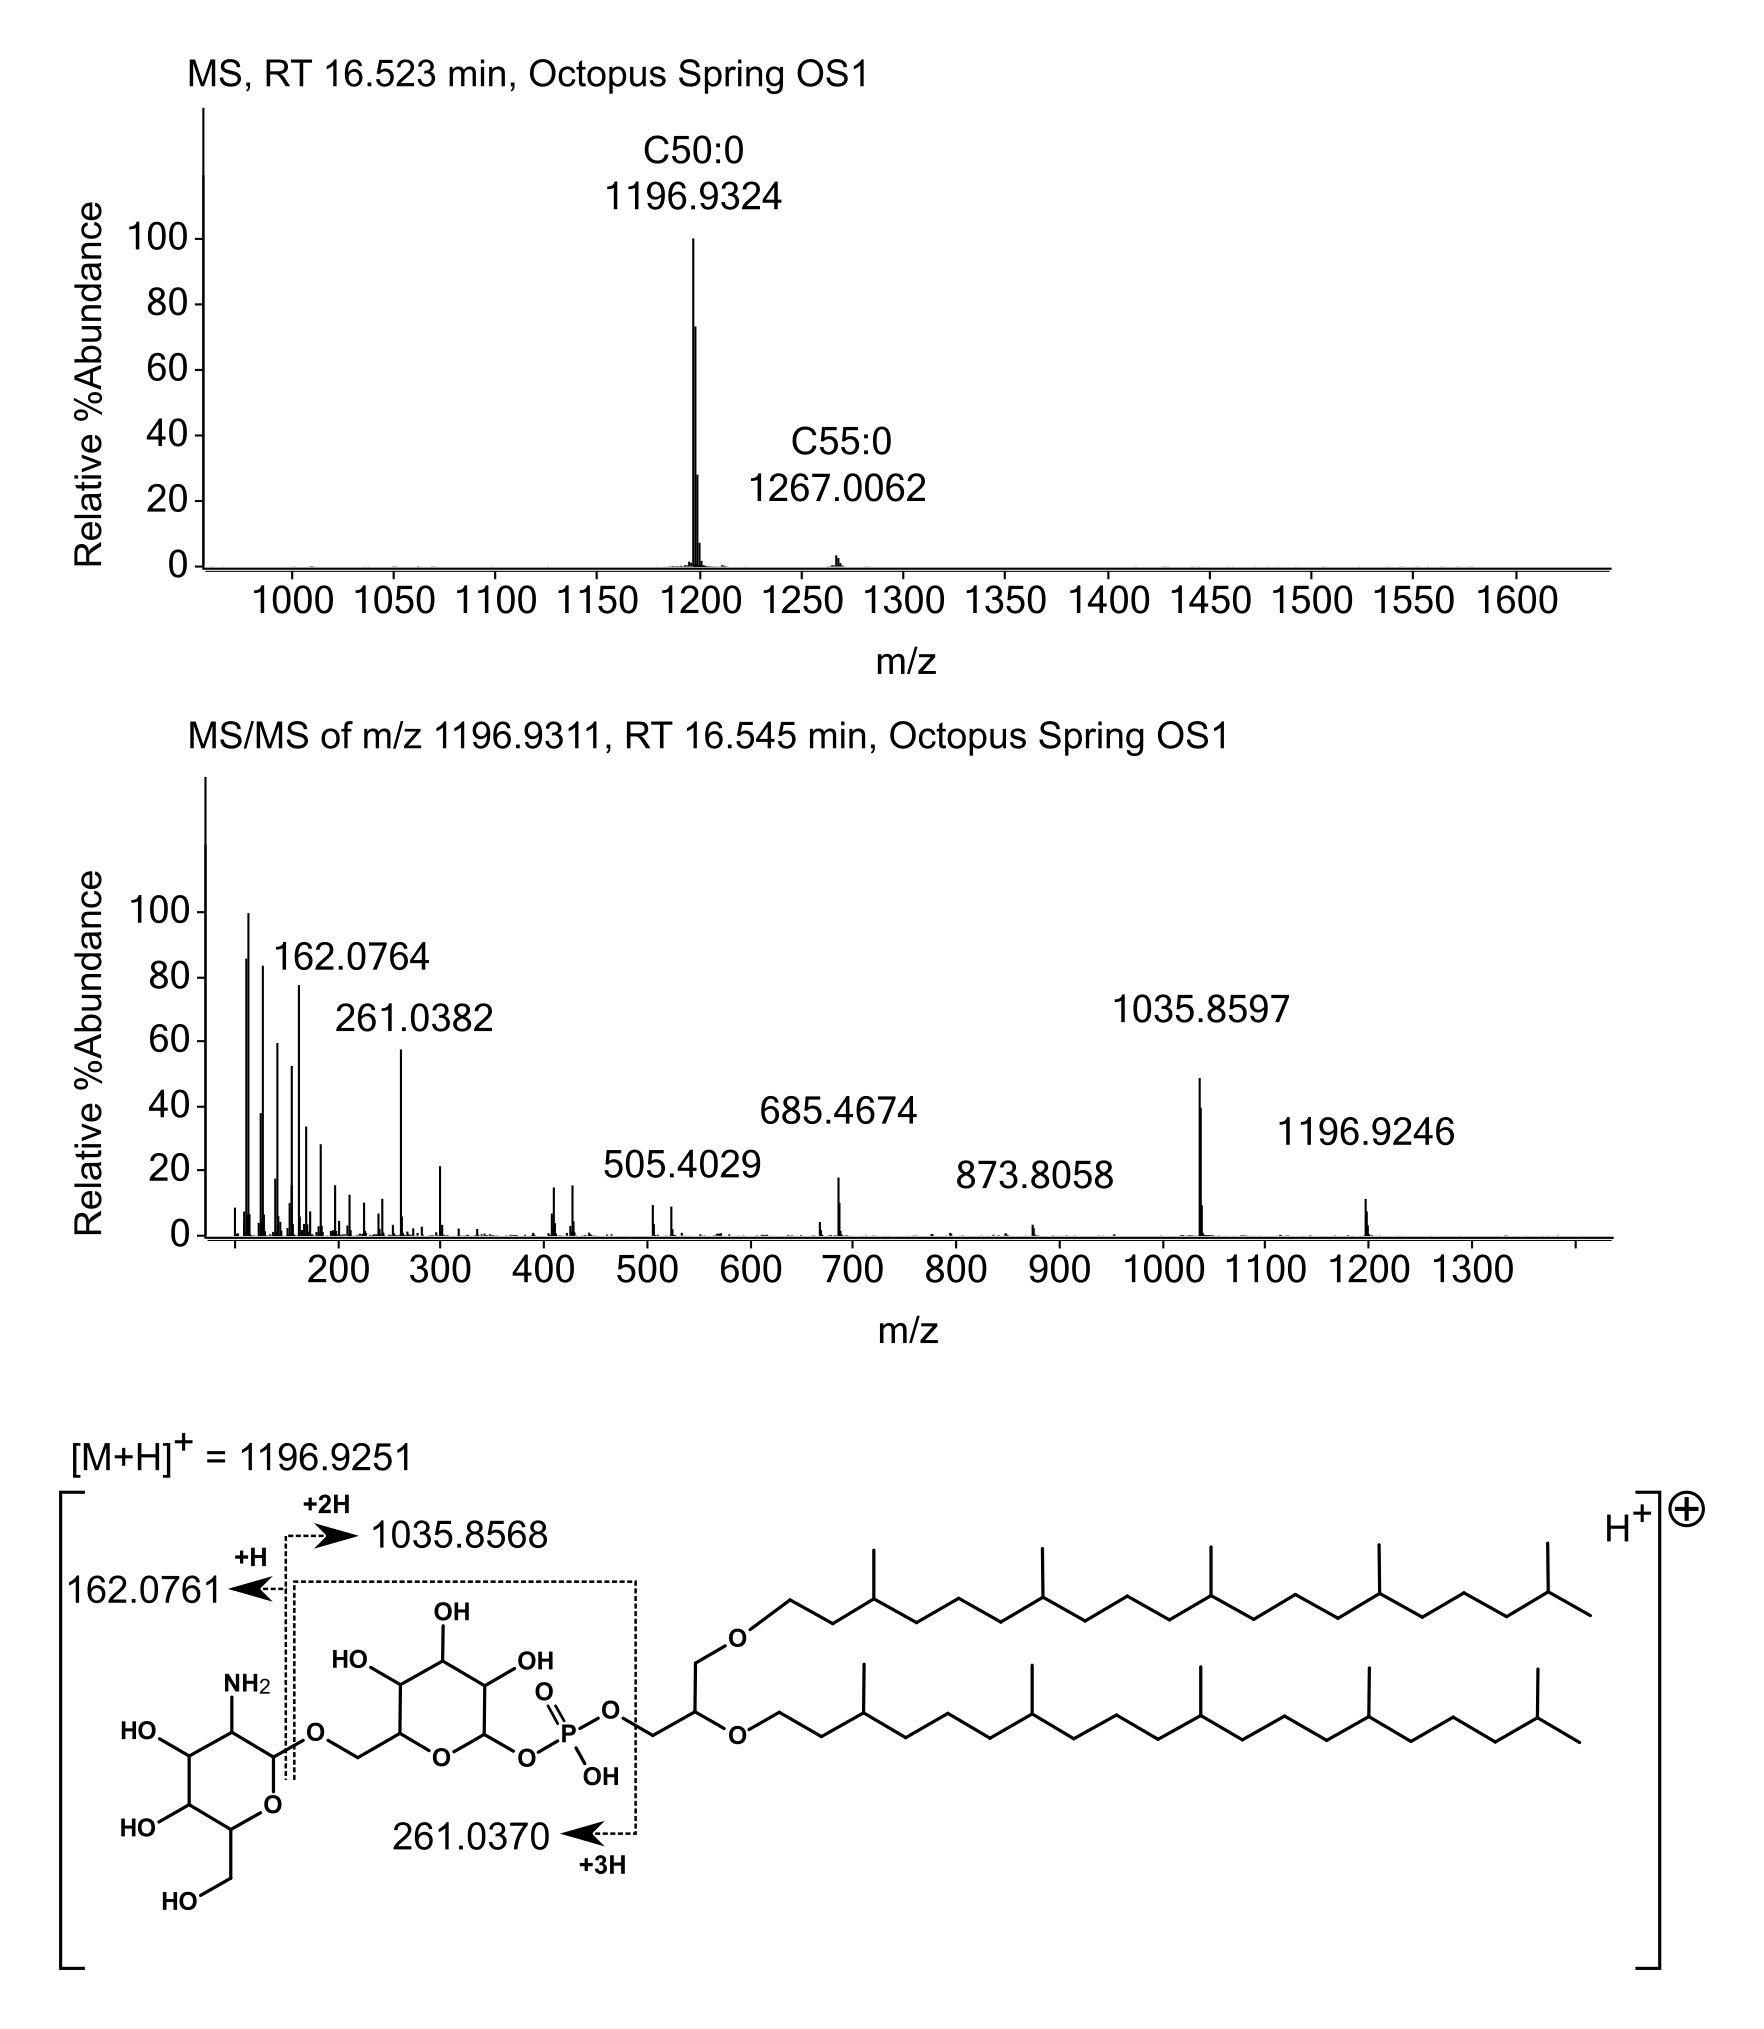
\includegraphics[width=\linewidth]{figs_app1/NG-G-P-AR}
\caption[Mass spectra and putative structure for (N)glycosaminyl monoglycosyl phosphatidylarchaeol (NG-G-P-AR)]{Mass spectra and putative structure for (N)glycosaminyl monoglycosyl phosphatidylarchaeol (NG-G-P-AR). This and MeNG-G-P-AR share many fragments in MS/MS due to their structural similarity (see Figure \ref{fig:MeNG-G-P-AR}).}
\label{fig:NG-G-P-AR_percent}
\end{figure}
\doublespace
\clearpage
}

\afterpage{
\singlespace
\begin{figure}[h]
\centering
\includegraphics[width=\linewidth]{figs_app1/TM-KL}
\caption{Mass spectrum and putative structure for (6-N,6-N,6-N)trimethyllysine lipid (TM-KL).}
\label{fig:TM-KL}
\end{figure}
\doublespace
\clearpage
}


\afterpage{
\singlespace
\begin{figure}[h]
\centering
\includegraphics[width=0.9\linewidth]{figs_app1/NG-GA-DAG}
\caption{Mass spectra and putative structure for (6-N,6-N,6-N)trimethyllysine lipid (NG-GA-DAG).}
\label{fig:NG-GA-DAG}
\end{figure}
\doublespace
\clearpage
}


\afterpage{
\singlespace
\begin{figure}[h]
\centering
    \begin{subfigure}[b]{1\linewidth}
       \includegraphics[width=\linewidth]{figs_app1/223-DAG_1}
       \caption{The MS/MS spectrum of C34:1 ‘223’-DAG within the m/z 250 – 800 range. Neutral loss of the headgroup results in [M + H]+ - m/z 223.07 = m/z 577.51, corresponding to the ion shown below, where nC in acyl chains R1 and R2 sum to 34 with one unsaturation.}
        \label{fig:223-DAG-MS}
    \end{subfigure}
\end{figure}
\newpage
\begin{figure}[h] \ContinuedFloat
    \begin{subfigure}[b]{1\linewidth}
       \includegraphics[width=\linewidth]{figs_app1/223-DAG_2}
       \caption{The MS/MS spectrum of C34:1 ‘223’-DAG within the m/z 140 – 250 range. The entire height of the 206 headgroup fragment is not shown. Dehydration reactions of base peak 206 results in: m/z 206.07 – 18.01 = m/z 188.06; m/z 206.07 – 2*18.01 = m/z 170.05; m/z 206.07 – 3*18.01 = m/z 152.04}
        \label{fig:223-DAG-structure}
    \end{subfigure}
\caption{Mass spectra and putative structure for unknown lipid `223'-DAG.}
\label{fig:223-DAG}
\end{figure}
\doublespace
\clearpage
}


\afterpage{
\singlespace
\begin{figure}[h]
\centering
\includegraphics[width=\linewidth]{figs_app1/G-MeNG-G-P-AR}
\caption{Mass spectrum and putative structure for glycosyl (N-methyl)glycosaminyl glycosyl phosphatidylarchaeol (G-MeNG-G-P-AR).}
\label{fig:G-MeNG-G-P-AR}
\end{figure}
\doublespace
\clearpage
}

\afterpage{
\singlespace
\begin{figure}[h]
\centering
\includegraphics[width=\linewidth]{figs_app1/G-NG-G-P-AR}
\caption[Mass spectra and putative structure for glycosyl (N)glycosaminyl glycosyl phosphatidylarchaeol (G-MeNG-G-P-AR)]{Mass spectra and putative structure for glycosyl (N)glycosaminyl glycosyl phosphatidylarchaeol (G-MeNG-G-P-AR). See Figure \ref{fig:MeNG-G-P-AR} for putative structures for fragments m/z 685 and 873.}
\label{fig:G-NG-G-P-AR}
\end{figure}
\doublespace
\clearpage
}


\afterpage{
\singlespace
\begin{figure}[h]
\centering
    \begin{subfigure}[b]{1\linewidth}
       \includegraphics[width=\linewidth]{figs_app1/3G-NAcG-G_1}
       \caption{}
        \label{fig:3G-NAcG-G-MS}
    \end{subfigure}
\end{figure}
\newpage
\begin{figure}[h] \ContinuedFloat
    \begin{subfigure}[b]{1\linewidth}
       \includegraphics[width=\linewidth]{figs_app1/3G-NAcG-G_2}
       \caption{}
        \label{fig:3G-NAcG-G-structure}
    \end{subfigure}
\caption[Mass spectra and putative structure for triglycosyl (N-acetyl)glycosaminyl glycosyl dietherglycerol (3G-NAcG-G-DEG)]{(\subref{fig:3G-NAcG-G-MS}) Mass spectra and (\subref{fig:3G-NAcG-G-structure}) putative structure for triglycosyl (N-acetyl)glycosaminyl glycosyl dietherglycerol (3G-NAcG-G-DEG).}
\label{fig:3G-NAcG-G}
\end{figure}
\doublespace
\clearpage
}

\afterpage{
\singlespace
\begin{figure}[h]
       \includegraphics[width=0.9\linewidth]{figs_app1/G-GA-DAG}
       \caption{Mass spectra and putative structure for G-GA-DAG.}
\label{fig:G-GA-DAG}
\end{figure}
\doublespace
\clearpage
}
\chapter{Supplementary figures: predicted metastable equilibrium abundances and sensitivity analyses of site-average free alkyl chains}

\begin{figure}[h]
\centering

    \begin{subfigure}[b]{\linewidth}
       	\includegraphics[width=1\linewidth]{"figs_app2/Mound OF1_thermo"}
       	\caption{MS1}
        \label{fig:MS1_thermo}
    \end{subfigure}
    \begin{subfigure}[b]{\linewidth}
    	\includegraphics[width=1\linewidth]{"figs_app2/Mound OF2_thermo"}
    	\caption{MS2}
        \label{fig:MS2_thermo}
    \end{subfigure}
    
\end{figure}

\newpage

\begin{figure}[h]\ContinuedFloat
\centering

    \begin{subfigure}[b]{\linewidth}
       	\includegraphics[width=1\linewidth]{"figs_app2/Mound OF3_thermo"}
       	\caption{MS3}
        \label{fig:MS3_thermo}
    \end{subfigure}
    \begin{subfigure}[b]{\linewidth}
    	\includegraphics[width=1\linewidth]{"figs_app2/Mound OF4_thermo"}
    	\caption{MS4}
        \label{fig:MS4_thermo}
    \end{subfigure}
    
\end{figure}

\newpage

\begin{figure}[h]\ContinuedFloat

    \begin{subfigure}[b]{\linewidth}
    	\includegraphics[width=\linewidth]{"figs_app2/Mound OF5_thermo"}
    	\caption{MS5}
        \label{fig:MS5_thermo}
    \end{subfigure}
    
    \caption{Metastable equilibrium percent abundance of sample-average free alkyl chains of Mound Spring predicted across an Eh gradient at the temperatures and bicarbonate, ammonium (or nitrate for MS5), and proton concentrations measured at (a) MS1, (b) MS2, (c) MS3, (d) MS4, and (e) MS5. The vertical dotted line indicates the lipid-predicted Eh of the sample.}
    \label{fig:MS_thermo}
\end{figure}

\begin{figure}[h]
\centering

    \begin{subfigure}[b]{\linewidth}
       	\includegraphics[width=1\linewidth]{"figs_app2/boxplot_ggplot_02bin Mound OF1 iter 999"}
       	\caption{MS1}
        \label{fig:MS1_mc}
    \end{subfigure}
    \begin{subfigure}[b]{\linewidth}
    	\includegraphics[width=1\linewidth]{"figs_app2/boxplot_ggplot_02bin Mound OF2 iter 999"}
    	\caption{MS2}
        \label{fig:MS2_mc}
    \end{subfigure}
    
\end{figure}

\newpage

\begin{figure}[h]\ContinuedFloat
\centering

    \begin{subfigure}[b]{\linewidth}
       	\includegraphics[width=1\linewidth]{"figs_app2/boxplot_ggplot_02bin Mound OF3 iter 999"}
       	\caption{MS3}
        \label{fig:MS3_mc}
    \end{subfigure}
    \begin{subfigure}[b]{\linewidth}
    	\includegraphics[width=1\linewidth]{"figs_app2/boxplot_ggplot_02bin Mound OF4 iter 999"}
    	\caption{MS4}
        \label{fig:MS4_mc}
    \end{subfigure}
    
\end{figure}

\newpage

\begin{figure}[h]\ContinuedFloat

    \begin{subfigure}[b]{\linewidth}
    	\includegraphics[width=\linewidth]{"figs_app2/boxplot_ggplot_02bin Mound OF5 iter 999"}
    	\caption{MS5}
        \label{fig:MS5_mc}
    \end{subfigure}
    
    \caption{Sensitivity analysis sample-average free alkyl chain metastable equilibrium percent abundance in Mound Spring samples (a) MS1, (b) MS2, (c) MS3, (d) MS4, and (e) MS5 after 999 iterations of Monte Carlo-style random variation of lipid HPLC peak areas by 30\% and mass spectral response factors between 0.01x and 100x. Results have a resolution of 400 calculations per iteration, binned here into 0.02 volt increments. Dark horizontal lines indicate median values for each distribution, with 50\% of the results around the median falling within the colored box (interquartile range, or IQR). Whiskers extend to an observation 1.5 times the IQR beyond this range. Values that fall outside the span of the whiskers are not indicated to reduce visual clutter.}
    \label{fig:MS_mc}
\end{figure}


\newpage

\begin{figure}[h]
\centering

    \begin{subfigure}[b]{\linewidth}
       	\includegraphics[width=1\linewidth]{"figs_app2/Empress OF1_thermo"}
       	\caption{EP1}
        \label{fig:EP1_thermo}
    \end{subfigure}
    \begin{subfigure}[b]{\linewidth}
    	\includegraphics[width=1\linewidth]{"figs_app2/Empress OF3_thermo"}
    	\caption{EP3}
        \label{fig:EP3_thermo}
    \end{subfigure}
    
\end{figure}

\newpage

\begin{figure}[h]\ContinuedFloat
\centering

    \begin{subfigure}[b]{\linewidth}
       	\includegraphics[width=1\linewidth]{"figs_app2/Empress OF4_thermo"}
       	\caption{EP4}
        \label{fig:EP4_thermo}
    \end{subfigure}
    \begin{subfigure}[b]{\linewidth}
    	\includegraphics[width=1\linewidth]{"figs_app2/Empress OF5_thermo"}
    	\caption{EP5}
        \label{fig:EP5_thermo}
    \end{subfigure}
    
    \caption{Metastable equilibrium percent abundance of sample-average free alkyl chains of Empress Pool predicted across an Eh gradient at the temperatures and bicarbonate, ammonium, and proton concentrations measured at (a) EP1, (b) EP3, (c) EP4, and (d) EP5. The vertical dotted line indicates the lipid-predicted Eh of the sample.}
    \label{fig:EP_thermo}
\end{figure}

\newpage

\begin{figure}[h]
\centering

    \begin{subfigure}[b]{\linewidth}
      	\includegraphics[width=1\linewidth]{"figs_app2/boxplot_ggplot_02bin Empress OF1 iter 999"}
      	\caption{EP1}
        \label{fig:EP1_mc}
    \end{subfigure}
    \begin{subfigure}[b]{\linewidth}
    	\includegraphics[width=1\linewidth]{"figs_app2/boxplot_ggplot_02bin Empress OF3 iter 999"}
    	\caption{EP3}
        \label{fig:EP3_mc}
    \end{subfigure}
    
\end{figure}

\newpage

\begin{figure}[h]\ContinuedFloat
\centering

    \begin{subfigure}[b]{\linewidth}
      	\includegraphics[width=1\linewidth]{"figs_app2/boxplot_ggplot_02bin Empress OF4 iter 999"}
      	\caption{EP4}
        \label{fig:EP4_mc}
    \end{subfigure}
    \begin{subfigure}[b]{\linewidth}
    	\includegraphics[width=1\linewidth]{"figs_app2/boxplot_ggplot_02bin Empress OF5 iter 999"}
    	\caption{EP5}
        \label{fig:EP5_mc}
    \end{subfigure}
    
    \caption{Sensitivity analysis sample-average free alkyl chain metastable equilibrium percent abundance in Empress Pool samples (a) EP1, (b) EP3, (c) EP4, and (d) EP5 after 999 iterations of Monte Carlo-style random variation of lipid HPLC peak areas by 30\% and mass spectral response factors between 0.01x and 100x. Results have a resolution of 400 calculations per iteration, binned here into 0.02 volt increments. Dark horizontal lines indicate median values for each distribution, with 50\% of the results around the median falling within the colored box (interquartile range, or IQR). Whiskers extend to an observation 1.5 times the IQR beyond this range. Values that fall outside the span of the whiskers are not indicated to reduce visual clutter.}
    \label{fig:EP_mc}
\end{figure}

\newpage

\begin{figure}[h]
\centering

    \begin{subfigure}[b]{\linewidth}
       	\includegraphics[width=1\linewidth]{"figs_app2/Octopus OF1_thermo"}
       	\caption{OS1}
        \label{fig:OS1_thermo}
    \end{subfigure}
    \begin{subfigure}[b]{\linewidth}
    	\includegraphics[width=1\linewidth]{"figs_app2/Octopus OF2_thermo"}
    	\caption{OS2}
        \label{fig:OS2_thermo}
    \end{subfigure}
    
    \caption{Metastable equilibrium percent abundance of sample-average free alkyl chains of Octopus Spring predicted across an Eh gradient at the temperatures and bicarbonate, ammonium, and proton concentrations measured at (a) OS1 and (b) OS2. The vertical dotted line indicates the lipid-predicted Eh of the sample.}
    \label{fig:OS_thermo}
\end{figure}

\newpage

\begin{figure}[h]
\centering

    \begin{subfigure}[b]{\linewidth}
      	\includegraphics[width=1\linewidth]{"figs_app2/boxplot_ggplot_02bin Octopus OF1 iter 999"}
      	\caption{OS1}
        \label{fig:OS1_mc}
    \end{subfigure}
    \begin{subfigure}[b]{\linewidth}
    	\includegraphics[width=1\linewidth]{"figs_app2/boxplot_ggplot_02bin Octopus OF2 iter 999"}
    	\caption{OS2}
        \label{fig:OS2_mc}
    \end{subfigure}

    
    \caption{Sensitivity analysis of sample-average free alkyl chain metastable equilibrium percent abundance in Empress Pool samples (a) OS1, and (b) OS2 after 999 iterations of Monte Carlo-style random variation of lipid HPLC peak areas by 30\% and mass spectral response factors between 0.01x and 100x. Results have a resolution of 400 calculations per iteration, binned here into 0.02 volt increments. Dark horizontal lines indicate median values for each distribution, with 50\% of the results around the median falling within the colored box (interquartile range, or IQR). Whiskers extend to an observation 1.5 times the IQR beyond this range. Values that fall outside the span of the whiskers are not indicated to reduce visual clutter.}
    \label{fig:OS_mc}
\end{figure}
\chapter{Supplementary figures: predicted equilibrium abundances of bacteriohopanepolyol polar headgroups}

\singlespace

\begin{figure}[h]
\centering
    \begin{subfigure}[b]{\linewidth}
        \includegraphics[width=\linewidth]{figs_app3/"Bison OF1_BHP_mosaic"}
        \label{fig:BP1_degform}
    \end{subfigure}
    \begin{subfigure}[b]{\linewidth}
        \includegraphics[width=\linewidth]{figs_app3/"Bison OF2_BHP_mosaic"}
        \label{fig:BP2_degform}
    \end{subfigure}
\end{figure}

\newpage

\begin{figure}[h]\ContinuedFloat
    \begin{subfigure}[b]{\linewidth}
        \includegraphics[width=\linewidth]{figs_app3/"Bison OF3_BHP_mosaic"}
        \label{fig:BP3_degform}
    \end{subfigure}\\[-4ex]
    \begin{subfigure}[b]{\linewidth}
    	\includegraphics[width=\linewidth]{figs_app3/"Bison OF4_BHP_mosaic"}
        \label{fig:BP4_degform}
    \end{subfigure}
\end{figure}

\newpage

\begin{figure}[h]\ContinuedFloat
    \begin{subfigure}[b]{\linewidth}
        \includegraphics[width=\linewidth]{figs_app3/"Bison OF5_BHP_mosaic"}
        \label{fig:BP5_degform}
    \end{subfigure}
    \begin{subfigure}[b]{\linewidth}
        \includegraphics[width=\linewidth]{figs_app3/"Bison OF6_BHP_mosaic"}
        \label{fig:BP6_degform}
    \end{subfigure}\\[-4ex]
\end{figure}

\newpage

\begin{figure}[h]\ContinuedFloat
    \begin{subfigure}[b]{\linewidth}
    	\includegraphics[width=\linewidth]{figs_app3/"Mound OF1_BHP_mosaic"}
        \label{fig:MS1_degform}
    \end{subfigure}
    \begin{subfigure}[b]{\linewidth}
        \includegraphics[width=\linewidth]{figs_app3/"Mound OF2_BHP_mosaic"}
        \label{fig:MS2_degform}
    \end{subfigure}
\end{figure}

\newpage

\begin{figure}[h]\ContinuedFloat
    \begin{subfigure}[b]{\linewidth}
        \includegraphics[width=\linewidth]{figs_app3/"Mound OF3_BHP_mosaic"}
        \label{fig:MS3_degform}
    \end{subfigure}\\[-4ex]
    \begin{subfigure}[b]{\linewidth}
    	\includegraphics[width=\linewidth]{figs_app3/"Mound OF4_BHP_mosaic"}
        \label{fig:MS4_degform}
    \end{subfigure}
\end{figure}

\newpage

\begin{figure}[h]\ContinuedFloat
    \begin{subfigure}[b]{\linewidth}
        \includegraphics[width=\linewidth]{figs_app3/"Mound OF5_BHP_mosaic"}
        \label{fig:MS5_degform}
    \end{subfigure}
    \begin{subfigure}[b]{\linewidth}
        \includegraphics[width=\linewidth]{figs_app3/"Empress OF1_BHP_mosaic"}
        \label{fig:EP1_degform}
    \end{subfigure}\\[-4ex]
\end{figure}

\newpage

\begin{figure}[h]\ContinuedFloat
    \begin{subfigure}[b]{\linewidth}
        \includegraphics[width=\linewidth]{figs_app3/"Empress OF3_BHP_mosaic"}
        \label{fig:EP3_degform}
    \end{subfigure}
    \begin{subfigure}[b]{\linewidth}
        \includegraphics[width=\linewidth]{figs_app3/"Empress OF4_BHP_mosaic"}
        \label{fig:EP4_degform}
    \end{subfigure}
\end{figure}

\newpage

\begin{figure}[h]\ContinuedFloat
    \begin{subfigure}[b]{\linewidth}
    	\includegraphics[width=\linewidth]{figs_app3/"Empress OF5_BHP_mosaic"}
        \label{fig:EP5_degform}
    \end{subfigure}\\[-4ex]
    \begin{subfigure}[b]{\linewidth}
        \includegraphics[width=\linewidth]{figs_app3/"Octopus OF1_BHP_mosaic"}
        \label{fig:OS1_degform}
    \end{subfigure}
\end{figure}

\newpage

\begin{figure}[h]\ContinuedFloat
    \begin{subfigure}[b]{\linewidth}
        \includegraphics[width=\linewidth]{figs_app3/"Octopus OF2_BHP_mosaic"}
        \label{fig:OS2_degform}
    \end{subfigure}\\[-4ex]

\caption[Predicted metastable equilibrium abundance of tetrafunctional and pentafunctional BHP headgroups in Mound Spring, Empress Pool, and Octopus Spring samples]{Predicted metastable equilibrium abundance of tetrafunctional (blue) and pentafunctional (orange) BHP headgroups in Mound Spring, Empress Pool, and Octopus Spring samples compared to observed ratios (blue to orange vertical arrow lengths) with corresponding BHP headgroup-predicted Eh indicated for each.}
\label{fig:degree_formation}
\end{figure}

\chapter{Thermodynamic equations of state}\label{app4}

\singlespace

% revised HKF equation
\begin{align} \label{eq:HKF_equation}
\begin{split}
\Delta G^{\circ}_{aq} = & \Delta_{f}G^{\circ}_{aq} - S_{aq}^{\circ}(T - T_{r}) - c_{1}\Big[T \cdot \ln{\frac{T}{T_{r}}} - T + T_{r} \Big] \\
      - & c_{2}\Big\{\Big[\Big(\frac{1}{T - \theta}\Big) - \Big(\frac{1}{T_{r} - \theta}\Big) \Big] \Big( \frac{\theta - T}{\theta} \Big) - \frac{T}{\theta^{2}} \ln{\Big( \frac{T_{r}(T - \theta)}{T(T_{r} - \theta)} \Big)} \Big\} \\
      + & a_{1}(P - P_{r}) + a_{2}\ln{\Big(\frac{\Psi + P}{\Psi + P_{r}} \Big)} + \Big( \frac{1}{T - \theta} \Big)\Big[ a_{3}(P - P_{r}) + a_{4}\ln{\Big( \frac{\Psi + P}{\Psi + P_{r}} \Big)} \Big] \\
      + & \omega \Big( \frac{1}{\epsilon} - 1 \Big)
\end{split}
\end{align}
\captionedequationset{The revised Helgeson-Kirkham-Flowers (HKF) equation of state used in this work was adapted from Equation B25 in \cite{shock1992calculation}. Solvation terms that were not expected to have a significant effect on results within the range of pressure and temperature considered in this study (1 bar and $<$ 100$^{\circ}$C) have been left out. $\Delta G^{\circ}_{aq}$ indicates the apparent standard partial molal Gibbs free energy of formation of the aqueous species from the elements at the temperature and pressure of interest. $S_{aq}^{\circ}$ and $\Delta_{f}G^{\circ}_{aq}$ stand for the standard partial molal entropy of the species and Gibbs free energy of formation of the aqueous species from the elements at 298.15K and 1 bar, respectively. $a_{1}$, $a_{2}$, $a_{3}$, $a_{4}$, $c_{1}$, $c_{2}$, and $\omega$ designate HKF equation of state parameters that are species-dependent. $T$ and $P$ stand for the temperature and pressure of interest. $T_{r}$ and $P_{r}$ represent the reference temperature and pressure, which are 298.15 K and 1 bar. $\theta$ and $\Psi$ designate solvent parameters equal to 228 K and 2600 bar, respectively. $\epsilon$ stands for the dielectric constant of water at the temperature and pressure of interest.}

\doublespace
\clearpage
\include{vita}
\end{document}
